\documentclass[twoside]{book}

% Packages required by doxygen
\usepackage{fixltx2e}
\usepackage{calc}
\usepackage{doxygen}
\usepackage[export]{adjustbox} % also loads graphicx
\usepackage{graphicx}
\usepackage[utf8]{inputenc}
\usepackage{makeidx}
\usepackage{multicol}
\usepackage{multirow}
\PassOptionsToPackage{warn}{textcomp}
\usepackage{textcomp}
\usepackage[nointegrals]{wasysym}
\usepackage[table]{xcolor}

% NLS support packages
\usepackage[french]{babel}

% Font selection
\usepackage[T1]{fontenc}
\usepackage[scaled=.90]{helvet}
\usepackage{courier}
\usepackage{amssymb}
\usepackage{sectsty}
\renewcommand{\familydefault}{\sfdefault}
\allsectionsfont{%
  \fontseries{bc}\selectfont%
  \color{darkgray}%
}
\renewcommand{\DoxyLabelFont}{%
  \fontseries{bc}\selectfont%
  \color{darkgray}%
}
\newcommand{\+}{\discretionary{\mbox{\scriptsize$\hookleftarrow$}}{}{}}

% Page & text layout
\usepackage{geometry}
\geometry{%
  a4paper,%
  top=2.5cm,%
  bottom=2.5cm,%
  left=2.5cm,%
  right=2.5cm%
}
\tolerance=750
\hfuzz=15pt
\hbadness=750
\setlength{\emergencystretch}{15pt}
\setlength{\parindent}{0cm}
\setlength{\parskip}{3ex plus 2ex minus 2ex}
\makeatletter
\renewcommand{\paragraph}{%
  \@startsection{paragraph}{4}{0ex}{-1.0ex}{1.0ex}{%
    \normalfont\normalsize\bfseries\SS@parafont%
  }%
}
\renewcommand{\subparagraph}{%
  \@startsection{subparagraph}{5}{0ex}{-1.0ex}{1.0ex}{%
    \normalfont\normalsize\bfseries\SS@subparafont%
  }%
}
\makeatother

% Headers & footers
\usepackage{fancyhdr}
\pagestyle{fancyplain}
\fancyhead[LE]{\fancyplain{}{\bfseries\thepage}}
\fancyhead[CE]{\fancyplain{}{}}
\fancyhead[RE]{\fancyplain{}{\bfseries\leftmark}}
\fancyhead[LO]{\fancyplain{}{\bfseries\rightmark}}
\fancyhead[CO]{\fancyplain{}{}}
\fancyhead[RO]{\fancyplain{}{\bfseries\thepage}}
\fancyfoot[LE]{\fancyplain{}{}}
\fancyfoot[CE]{\fancyplain{}{}}
\fancyfoot[RE]{\fancyplain{}{\bfseries\scriptsize Généré par Doxygen }}
\fancyfoot[LO]{\fancyplain{}{\bfseries\scriptsize Généré par Doxygen }}
\fancyfoot[CO]{\fancyplain{}{}}
\fancyfoot[RO]{\fancyplain{}{}}
\renewcommand{\footrulewidth}{0.4pt}
\renewcommand{\chaptermark}[1]{%
  \markboth{#1}{}%
}
\renewcommand{\sectionmark}[1]{%
  \markright{\thesection\ #1}%
}

% Indices & bibliography
\usepackage{natbib}
\usepackage[titles]{tocloft}
\setcounter{tocdepth}{3}
\setcounter{secnumdepth}{5}
\makeindex

% Hyperlinks (required, but should be loaded last)
\usepackage{ifpdf}
\ifpdf
  \usepackage[pdftex,pagebackref=true]{hyperref}
\else
  \usepackage[ps2pdf,pagebackref=true]{hyperref}
\fi
\hypersetup{%
  colorlinks=true,%
  linkcolor=blue,%
  citecolor=blue,%
  unicode%
}

% Custom commands
\newcommand{\clearemptydoublepage}{%
  \newpage{\pagestyle{empty}\cleardoublepage}%
}

\usepackage{caption}
\captionsetup{labelsep=space,justification=centering,font={bf},singlelinecheck=off,skip=4pt,position=top}

%===== C O N T E N T S =====

\begin{document}

% Titlepage & ToC
\hypersetup{pageanchor=false,
             bookmarksnumbered=true,
             pdfencoding=unicode
            }
\pagenumbering{alph}
\begin{titlepage}
\vspace*{7cm}
\begin{center}%
{\Large Hand\+Over Tools }\\
\vspace*{1cm}
{\large Généré par Doxygen 1.8.13}\\
\end{center}
\end{titlepage}
\clearemptydoublepage
\pagenumbering{roman}
\tableofcontents
\clearemptydoublepage
\pagenumbering{arabic}
\hypersetup{pageanchor=true}

%--- Begin generated contents ---
\chapter{Index des espaces de nommage}
\section{Liste des espaces de nommage}
Liste de tous les espaces de nommage avec une brève description\+:\begin{DoxyCompactList}
\item\contentsline{section}{\hyperlink{namespaceScript}{Script} }{\pageref{namespaceScript}}{}
\item\contentsline{section}{\hyperlink{namespaceScript_1_1handOver}{Script.\+hand\+Over} }{\pageref{namespaceScript_1_1handOver}}{}
\item\contentsline{section}{\hyperlink{namespaceScript_1_1interfaceFrame}{Script.\+interface\+Frame} }{\pageref{namespaceScript_1_1interfaceFrame}}{}
\item\contentsline{section}{\hyperlink{namespaceScript_1_1omc}{Script.\+omc} }{\pageref{namespaceScript_1_1omc}}{}
\item\contentsline{section}{\hyperlink{namespaceScript_1_1omu}{Script.\+omu} }{\pageref{namespaceScript_1_1omu}}{}
\item\contentsline{section}{\hyperlink{namespaceScript_1_1Option}{Script.\+Option} }{\pageref{namespaceScript_1_1Option}}{}
\item\contentsline{section}{\hyperlink{namespaceScript_1_1progress__bar}{Script.\+progress\+\_\+bar} }{\pageref{namespaceScript_1_1progress__bar}}{}
\item\contentsline{section}{\hyperlink{namespaceScript_1_1Setup}{Script.\+Setup} }{\pageref{namespaceScript_1_1Setup}}{}
\end{DoxyCompactList}

\chapter{Index hiérarchique}
\section{Hiérarchie des classes}
Cette liste d\textquotesingle{}héritage est classée approximativement par ordre alphabétique \+:\begin{DoxyCompactList}
\item Frame\begin{DoxyCompactList}
\item \contentsline{section}{Script.\+Setup.\+Main\+Interface}{\pageref{classScript_1_1Setup_1_1MainInterface}}{}
\end{DoxyCompactList}
\item \contentsline{section}{Script.\+omc.\+O\+MC}{\pageref{classScript_1_1omc_1_1OMC}}{}
\item \contentsline{section}{Script.\+omu.\+O\+MU}{\pageref{classScript_1_1omu_1_1OMU}}{}
\item Tk\begin{DoxyCompactList}
\item \contentsline{section}{Script.\+progress\+\_\+bar.\+Sample\+App}{\pageref{classScript_1_1progress__bar_1_1SampleApp}}{}
\end{DoxyCompactList}
\item Thread\begin{DoxyCompactList}
\item \contentsline{section}{Script.\+hand\+Over.\+Mobile\+Receives}{\pageref{classScript_1_1handOver_1_1MobileReceives}}{}
\item \contentsline{section}{Script.\+hand\+Over.\+Mobile\+Transmitter}{\pageref{classScript_1_1handOver_1_1MobileTransmitter}}{}
\end{DoxyCompactList}
\end{DoxyCompactList}

\chapter{Index des classes}
\section{Liste des classes}
Liste des classes, structures, unions et interfaces avec une brève description \+:\begin{DoxyCompactList}
\item\contentsline{section}{\hyperlink{classScript_1_1Setup_1_1MainInterface}{Script.\+Setup.\+Main\+Interface} }{\pageref{classScript_1_1Setup_1_1MainInterface}}{}
\item\contentsline{section}{\hyperlink{classScript_1_1handOver_1_1MobileReceives}{Script.\+hand\+Over.\+Mobile\+Receives} }{\pageref{classScript_1_1handOver_1_1MobileReceives}}{}
\item\contentsline{section}{\hyperlink{classScript_1_1handOver_1_1MobileTransmitter}{Script.\+hand\+Over.\+Mobile\+Transmitter} }{\pageref{classScript_1_1handOver_1_1MobileTransmitter}}{}
\item\contentsline{section}{\hyperlink{classScript_1_1omc_1_1OMC}{Script.\+omc.\+O\+MC} }{\pageref{classScript_1_1omc_1_1OMC}}{}
\item\contentsline{section}{\hyperlink{classScript_1_1omu_1_1OMU}{Script.\+omu.\+O\+MU} }{\pageref{classScript_1_1omu_1_1OMU}}{}
\item\contentsline{section}{\hyperlink{classScript_1_1progress__bar_1_1SampleApp}{Script.\+progress\+\_\+bar.\+Sample\+App} }{\pageref{classScript_1_1progress__bar_1_1SampleApp}}{}
\end{DoxyCompactList}

\chapter{Index des fichiers}
\section{Liste des fichiers}
Liste de tous les fichiers avec une brève description \+:\begin{DoxyCompactList}
\item\contentsline{section}{\hyperlink{____init_____8py}{\+\_\+\+\_\+init\+\_\+\+\_\+.\+py} }{\pageref{____init_____8py}}{}
\item\contentsline{section}{\hyperlink{handOver_8py}{hand\+Over.\+py} }{\pageref{handOver_8py}}{}
\item\contentsline{section}{\hyperlink{interfaceFrame_8py}{interface\+Frame.\+py} }{\pageref{interfaceFrame_8py}}{}
\item\contentsline{section}{\hyperlink{omc_8py}{omc.\+py} }{\pageref{omc_8py}}{}
\item\contentsline{section}{\hyperlink{omu_8py}{omu.\+py} }{\pageref{omu_8py}}{}
\item\contentsline{section}{\hyperlink{Option_8py}{Option.\+py} }{\pageref{Option_8py}}{}
\item\contentsline{section}{\hyperlink{progress__bar_8py}{progress\+\_\+bar.\+py} }{\pageref{progress__bar_8py}}{}
\item\contentsline{section}{\hyperlink{Setup_8py}{Setup.\+py} }{\pageref{Setup_8py}}{}
\end{DoxyCompactList}

\chapter{Documentation des espaces de nommage}
\hypertarget{namespaceScript}{}\section{Référence de l\textquotesingle{}espace de nommage Script}
\label{namespaceScript}\index{Script@{Script}}
\subsection*{Espaces de nommage}
\begin{DoxyCompactItemize}
\item 
 \hyperlink{namespaceScript_1_1handOver}{hand\+Over}
\item 
 \hyperlink{namespaceScript_1_1interfaceFrame}{interface\+Frame}
\item 
 \hyperlink{namespaceScript_1_1omc}{omc}
\item 
 \hyperlink{namespaceScript_1_1omu}{omu}
\item 
 \hyperlink{namespaceScript_1_1Option}{Option}
\item 
 \hyperlink{namespaceScript_1_1progress__bar}{progress\+\_\+bar}
\item 
 \hyperlink{namespaceScript_1_1Setup}{Setup}
\end{DoxyCompactItemize}

\hypertarget{namespaceScript_1_1handOver}{}\section{Référence de l\textquotesingle{}espace de nommage Script.\+hand\+Over}
\label{namespaceScript_1_1handOver}\index{Script.\+hand\+Over@{Script.\+hand\+Over}}
\subsection*{Classes}
\begin{DoxyCompactItemize}
\item 
class \hyperlink{classScript_1_1handOver_1_1MobileReceives}{Mobile\+Receives}
\item 
class \hyperlink{classScript_1_1handOver_1_1MobileTransmitter}{Mobile\+Transmitter}
\end{DoxyCompactItemize}
\subsection*{Fonctions}
\begin{DoxyCompactItemize}
\item 
def \hyperlink{namespaceScript_1_1handOver_a4d9a0e646528d168d925b4bcd6f078a6}{begin\+\_\+hand\+Over} (simple, tmu, ptp, data, vgcs, rec, vbs)
\end{DoxyCompactItemize}
\subsection*{Variables}
\begin{DoxyCompactItemize}
\item 
\hyperlink{namespaceScript_1_1handOver_a94f94a457b98f7aa4528c5118490f262}{V\+E\+R\+R\+OU} = R\+Lock()
\item 
bool \hyperlink{namespaceScript_1_1handOver_a1f8a11e1df500a2ab144549e8f3e4703}{C\+O\+N\+F\+I\+RM} = True
\item 
int \hyperlink{namespaceScript_1_1handOver_a10996755a745f6ffa98a8c5235d8d4b3}{baudrate} = 9600
\end{DoxyCompactItemize}


\subsection{Documentation des fonctions}
\mbox{\Hypertarget{namespaceScript_1_1handOver_a4d9a0e646528d168d925b4bcd6f078a6}\label{namespaceScript_1_1handOver_a4d9a0e646528d168d925b4bcd6f078a6}} 
\index{Script\+::hand\+Over@{Script\+::hand\+Over}!begin\+\_\+hand\+Over@{begin\+\_\+hand\+Over}}
\index{begin\+\_\+hand\+Over@{begin\+\_\+hand\+Over}!Script\+::hand\+Over@{Script\+::hand\+Over}}
\subsubsection{\texorpdfstring{begin\+\_\+hand\+Over()}{begin\_handOver()}}
{\footnotesize\ttfamily def Script.\+hand\+Over.\+begin\+\_\+hand\+Over (\begin{DoxyParamCaption}\item[{}]{simple,  }\item[{}]{tmu,  }\item[{}]{ptp,  }\item[{}]{data,  }\item[{}]{vgcs,  }\item[{}]{rec,  }\item[{}]{vbs }\end{DoxyParamCaption})}



Définition à la ligne 28 du fichier hand\+Over.\+py.


\begin{DoxyCode}
28 \textcolor{keyword}{def }\hyperlink{namespaceScript_1_1handOver_a4d9a0e646528d168d925b4bcd6f078a6}{begin\_handOver}(simple, tmu, ptp, data, vgcs, rec, vbs):
29     \textcolor{keyword}{global} RING\_STATUS
30     Option.RUNNING= \textcolor{keyword}{True}
31     RING\_STATUS= \textcolor{keyword}{False}
32     Option.progress\_Bar()
33     thread\_receives=MobileReceives()
34     thread\_transmitter= MobileTransmitter(simple, tmu, ptp, data, vgcs, rec, vbs)
35     thread\_receives.start()
36     thread\_transmitter.start()
37 
38 
39     \textcolor{comment}{#thread\_limit\_waiting= Thread(target= Option.limit\_waiting)
}
40     \textcolor{comment}{#thread\_limit\_waiting.start()
}
41 
42 \textcolor{comment}{# Cette classe permet de configure le mobile qui réçoit l'appel
}
43 \textcolor{comment}{# elle confire tout abord le mobile à une vitesse que l'utilisateur à definie, cela permet à mieux
       d'etablir un appel
}
44 \textcolor{comment}{# elle se met a l'ecoute et est capable de crocher un appel ou raccrocher un appel de type groupe call
}
\end{DoxyCode}


\subsection{Documentation des variables}
\mbox{\Hypertarget{namespaceScript_1_1handOver_a10996755a745f6ffa98a8c5235d8d4b3}\label{namespaceScript_1_1handOver_a10996755a745f6ffa98a8c5235d8d4b3}} 
\index{Script\+::hand\+Over@{Script\+::hand\+Over}!baudrate@{baudrate}}
\index{baudrate@{baudrate}!Script\+::hand\+Over@{Script\+::hand\+Over}}
\subsubsection{\texorpdfstring{baudrate}{baudrate}}
{\footnotesize\ttfamily int Script.\+hand\+Over.\+baudrate = 9600}



Définition à la ligne 24 du fichier hand\+Over.\+py.

\mbox{\Hypertarget{namespaceScript_1_1handOver_a1f8a11e1df500a2ab144549e8f3e4703}\label{namespaceScript_1_1handOver_a1f8a11e1df500a2ab144549e8f3e4703}} 
\index{Script\+::hand\+Over@{Script\+::hand\+Over}!C\+O\+N\+F\+I\+RM@{C\+O\+N\+F\+I\+RM}}
\index{C\+O\+N\+F\+I\+RM@{C\+O\+N\+F\+I\+RM}!Script\+::hand\+Over@{Script\+::hand\+Over}}
\subsubsection{\texorpdfstring{C\+O\+N\+F\+I\+RM}{CONFIRM}}
{\footnotesize\ttfamily bool Script.\+hand\+Over.\+C\+O\+N\+F\+I\+RM = True}



Définition à la ligne 23 du fichier hand\+Over.\+py.

\mbox{\Hypertarget{namespaceScript_1_1handOver_a94f94a457b98f7aa4528c5118490f262}\label{namespaceScript_1_1handOver_a94f94a457b98f7aa4528c5118490f262}} 
\index{Script\+::hand\+Over@{Script\+::hand\+Over}!V\+E\+R\+R\+OU@{V\+E\+R\+R\+OU}}
\index{V\+E\+R\+R\+OU@{V\+E\+R\+R\+OU}!Script\+::hand\+Over@{Script\+::hand\+Over}}
\subsubsection{\texorpdfstring{V\+E\+R\+R\+OU}{VERROU}}
{\footnotesize\ttfamily Script.\+hand\+Over.\+V\+E\+R\+R\+OU = R\+Lock()}



Définition à la ligne 18 du fichier hand\+Over.\+py.


\hypertarget{namespaceScript_1_1interfaceFrame}{}\section{Référence de l\textquotesingle{}espace de nommage Script.\+interface\+Frame}
\label{namespaceScript_1_1interfaceFrame}\index{Script.\+interface\+Frame@{Script.\+interface\+Frame}}
\subsection*{Fonctions}
\begin{DoxyCompactItemize}
\item 
def \hyperlink{namespaceScript_1_1interfaceFrame_aa7f559f2c9e8af048daa456cb3686155}{Frame\+\_\+init\+\_\+option} (self, other\+Frame2, other\+Frame3)
\item 
def \hyperlink{namespaceScript_1_1interfaceFrame_a3538cb8357b74776a380240ed3221bc0}{Frame\+\_\+select\+\_\+com} (self, val\+\_\+type)
\item 
def \hyperlink{namespaceScript_1_1interfaceFrame_ae94a2df22674070fddf2ae5197a09a6f}{Frame\+\_\+btn\+\_\+execution} (self)
\item 
def \hyperlink{namespaceScript_1_1interfaceFrame_a76119121c3aceb43846ba3ea526623ad}{Scan\+\_\+com} ()
\item 
def \hyperlink{namespaceScript_1_1interfaceFrame_a7a90dd83e0b67edcf2dee870d927e98e}{verif\+\_\+args} ()
\item 
def \hyperlink{namespaceScript_1_1interfaceFrame_ab554e77db5080fb2eae78e39ebbeb395}{split\+\_\+chaine} (chaine, caractere)
\end{DoxyCompactItemize}
\subsection*{Variables}
\begin{DoxyCompactItemize}
\item 
\hyperlink{namespaceScript_1_1interfaceFrame_ab8e385a4d6a1f87628b963bc0a385519}{begin\+\_\+time} = time.\+time()
\item 
int \hyperlink{namespaceScript_1_1interfaceFrame_ace1207561541cc3ee3af9b2f33b2a316}{val\+\_\+line} = 0
\item 
string \hyperlink{namespaceScript_1_1interfaceFrame_a2cfacdb24b52e8cf5d9667d91a5c58ab}{V\+A\+L\+U\+E\+\_\+\+F\+I\+L\+E\+\_\+\+C\+O\+NF} = \char`\"{}\char`\"{}
\item 
string \hyperlink{namespaceScript_1_1interfaceFrame_a3704b57444e587c904b839d2dfef2b7e}{V\+A\+L\+U\+E\+\_\+\+F\+I\+L\+E\+\_\+\+C\+MD} = \char`\"{}\char`\"{}
\item 
string \hyperlink{namespaceScript_1_1interfaceFrame_a8933d662775f7e5fc3e0b8e5fb499b24}{V\+A\+L\+U\+E\+\_\+\+F\+I\+L\+E\+\_\+\+S\+A\+VE} = \char`\"{}\char`\"{}
\item 
string \hyperlink{namespaceScript_1_1interfaceFrame_a235ac21d18cefa672100db29db0ed490}{V\+A\+L\+U\+E\+\_\+\+F\+I\+L\+E\+\_\+\+A\+U\+D\+IO} = \char`\"{}\char`\"{}
\end{DoxyCompactItemize}


\subsection{Documentation des fonctions}
\mbox{\Hypertarget{namespaceScript_1_1interfaceFrame_ae94a2df22674070fddf2ae5197a09a6f}\label{namespaceScript_1_1interfaceFrame_ae94a2df22674070fddf2ae5197a09a6f}} 
\index{Script\+::interface\+Frame@{Script\+::interface\+Frame}!Frame\+\_\+btn\+\_\+execution@{Frame\+\_\+btn\+\_\+execution}}
\index{Frame\+\_\+btn\+\_\+execution@{Frame\+\_\+btn\+\_\+execution}!Script\+::interface\+Frame@{Script\+::interface\+Frame}}
\subsubsection{\texorpdfstring{Frame\+\_\+btn\+\_\+execution()}{Frame\_btn\_execution()}}
{\footnotesize\ttfamily def Script.\+interface\+Frame.\+Frame\+\_\+btn\+\_\+execution (\begin{DoxyParamCaption}\item[{}]{self }\end{DoxyParamCaption})}



Définition à la ligne 307 du fichier interface\+Frame.\+py.



Références Script.\+interface\+Frame.\+verif\+\_\+args().


\begin{DoxyCode}
307 \textcolor{keyword}{def }\hyperlink{namespaceScript_1_1interfaceFrame_ae94a2df22674070fddf2ae5197a09a6f}{Frame\_btn\_execution}(self):
308     self= Frame(self)
309     self.pack(side=TOP, padx=5, pady=5)
310     bouton\_exec= Button(self,width=10, text=\textcolor{stringliteral}{"Exécute"}, command=\textcolor{keyword}{lambda}:\hyperlink{namespaceScript_1_1interfaceFrame_a7a90dd83e0b67edcf2dee870d927e98e}{verif\_args}())
311     bouton\_exec.grid(column=3, row=0,)
312 
313 
314 \textcolor{comment}{# elle scan la liste des comme disponible sur la machine
}
315 \textcolor{comment}{# neamoins cette fonction ne vous permet de savoir quelle COM correspond à quel mobile
}
316 \textcolor{comment}{# donc vous devez quand même savoir par d'autres les COM de vos mobiles
}
\end{DoxyCode}
Voici le graphe d\textquotesingle{}appel pour cette fonction \+:\nopagebreak
\begin{figure}[H]
\begin{center}
\leavevmode
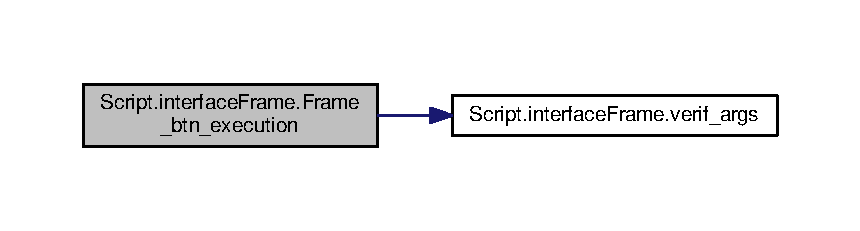
\includegraphics[width=350pt]{namespaceScript_1_1interfaceFrame_ae94a2df22674070fddf2ae5197a09a6f_cgraph}
\end{center}
\end{figure}
\mbox{\Hypertarget{namespaceScript_1_1interfaceFrame_aa7f559f2c9e8af048daa456cb3686155}\label{namespaceScript_1_1interfaceFrame_aa7f559f2c9e8af048daa456cb3686155}} 
\index{Script\+::interface\+Frame@{Script\+::interface\+Frame}!Frame\+\_\+init\+\_\+option@{Frame\+\_\+init\+\_\+option}}
\index{Frame\+\_\+init\+\_\+option@{Frame\+\_\+init\+\_\+option}!Script\+::interface\+Frame@{Script\+::interface\+Frame}}
\subsubsection{\texorpdfstring{Frame\+\_\+init\+\_\+option()}{Frame\_init\_option()}}
{\footnotesize\ttfamily def Script.\+interface\+Frame.\+Frame\+\_\+init\+\_\+option (\begin{DoxyParamCaption}\item[{}]{self,  }\item[{}]{other\+Frame2,  }\item[{}]{other\+Frame3 }\end{DoxyParamCaption})}



Définition à la ligne 56 du fichier interface\+Frame.\+py.


\begin{DoxyCode}
56 \textcolor{keyword}{def }\hyperlink{namespaceScript_1_1interfaceFrame_aa7f559f2c9e8af048daa456cb3686155}{Frame\_init\_option}(self, otherFrame2 ,otherFrame3):
57     \textcolor{keyword}{global} VALUE\_SELECT\_CALL\_OPTION
58     \textcolor{keyword}{global} VALUE\_SELECT\_CALL\_CONFIG
59     VALUE\_SELECT\_CALL\_OPTION=\{\}
60     VALUE\_SELECT\_CALL\_CONFIG=\{\}
61 
62     labelFrame= LabelFrame(self, text=\textcolor{stringliteral}{"CONFIG HandOver"},borderwidth=10, relief=GROOVE)
63     labelFrame.pack(side=TOP, padx=10, pady=5)
64 
65     labelFrame1= LabelFrame(labelFrame, text=\textcolor{stringliteral}{"HandOver Type"},borderwidth=5, relief=GROOVE)
66     labelFrame1.grid(column=0,row=0,padx=14, pady=2)
67 
68     labelFrame2= LabelFrame(labelFrame, text=\textcolor{stringliteral}{"Type of call"},borderwidth=5, relief=GROOVE)
69     labelFrame2.grid(column=1,row=0,padx=14, pady=2)
70 
71     call\_config=[\textcolor{stringliteral}{"SIMPLE"},\textcolor{stringliteral}{"RESET-TMU"}]
72     call\_modes=[\textcolor{stringliteral}{"PTP"},\textcolor{stringliteral}{"DATA"},\textcolor{stringliteral}{"VGCS"},\textcolor{stringliteral}{"REC"},\textcolor{stringliteral}{"VBS"}]
73 
74     j= 0
75 
76     \textcolor{keywordflow}{for} text \textcolor{keywordflow}{in} call\_config:
77         var\_call\_config = IntVar()
78         var\_call\_config.set(1)
79         VALUE\_SELECT\_CALL\_CONFIG[text]= var\_call\_config
80         bouton= ttk.Checkbutton(labelFrame1, text=text, variable=VALUE\_SELECT\_CALL\_CONFIG[text])
81         bouton.state([\textcolor{stringliteral}{'!disabled'},\textcolor{stringliteral}{'selected'}])
82         bouton.grid(row=j, padx= 35,sticky=W)
83         j+=1
84     j= 0
85     \textcolor{keywordflow}{for} text \textcolor{keywordflow}{in} call\_modes:
86         var\_select = IntVar()
87         var\_select.set(1)
88 
89         VALUE\_SELECT\_CALL\_OPTION[text]= var\_select
90         bouton= ttk.Checkbutton(labelFrame2, text=text, variable=VALUE\_SELECT\_CALL\_OPTION[text])
91         bouton.state([\textcolor{stringliteral}{'!disabled'},\textcolor{stringliteral}{'selected'}])
92         bouton.grid(row=j, padx= 35,sticky=W)
93         j+=1
94 \textcolor{stringliteral}{"""
}
95 \textcolor{stringliteral}{c'est la deuxieme frame de la frame principale,
}
96 \textcolor{stringliteral}{elle change en fonction des differentss selection de l'utilisateur depuis de la frame\_init\_option
}
97 \textcolor{stringliteral}{a chaque selection elle intialise le champs option necessaire pour l'excution du programme 
}
98 \textcolor{stringliteral}{
}
99 \textcolor{stringliteral}{"""}
100 \textcolor{comment}{# c'est la partie qui correspond au champ de selection des com des téléphone mobile
}
101 \textcolor{comment}{# elle permet également de saisir des information comme le numéro du mobile qui réçois l'appel ou le champ
       qui correpond au groupe ID
}
\end{DoxyCode}
\mbox{\Hypertarget{namespaceScript_1_1interfaceFrame_a3538cb8357b74776a380240ed3221bc0}\label{namespaceScript_1_1interfaceFrame_a3538cb8357b74776a380240ed3221bc0}} 
\index{Script\+::interface\+Frame@{Script\+::interface\+Frame}!Frame\+\_\+select\+\_\+com@{Frame\+\_\+select\+\_\+com}}
\index{Frame\+\_\+select\+\_\+com@{Frame\+\_\+select\+\_\+com}!Script\+::interface\+Frame@{Script\+::interface\+Frame}}
\subsubsection{\texorpdfstring{Frame\+\_\+select\+\_\+com()}{Frame\_select\_com()}}
{\footnotesize\ttfamily def Script.\+interface\+Frame.\+Frame\+\_\+select\+\_\+com (\begin{DoxyParamCaption}\item[{}]{self,  }\item[{}]{val\+\_\+type }\end{DoxyParamCaption})}



Définition à la ligne 102 du fichier interface\+Frame.\+py.



Références Script.\+interface\+Frame.\+Scan\+\_\+com().


\begin{DoxyCode}
102 \textcolor{keyword}{def }\hyperlink{namespaceScript_1_1interfaceFrame_a3538cb8357b74776a380240ed3221bc0}{Frame\_select\_com}(self, val\_type):
103     \textcolor{keyword}{global} VALUE\_BOX\_COM1 
104     \textcolor{keyword}{global} VALUE\_BOX\_COM2
105     \textcolor{keyword}{global} VALUE\_ENTRY\_PHONE\_NUMERO
106     \textcolor{keyword}{global} VALUE\_ENTRY\_ATCBST
107     \textcolor{keyword}{global} VALUE\_ENTRY\_GROUP\_ID
108 
109     \textcolor{keyword}{global} VALUE\_ENTRY\_OMC\_IP
110     \textcolor{keyword}{global} VALUE\_ENTRY\_OMC\_PASSWORD
111     \textcolor{keyword}{global} VALUE\_ENTRY\_OMC\_USER
112 
113     \textcolor{keyword}{global} VALUE\_ENTRY\_OMU1\_IP
114     \textcolor{keyword}{global} VALUE\_ENTRY\_OMU1\_PASSWORD
115     \textcolor{keyword}{global} VALUE\_ENTRY\_OMU1\_USER
116 
117     \textcolor{keyword}{global} VALUE\_ENTRY\_OMU2\_IP
118     \textcolor{keyword}{global} VALUE\_ENTRY\_OMU2\_PASSWORD
119     \textcolor{keyword}{global} VALUE\_ENTRY\_OMU2\_USER
120     \textcolor{keyword}{global} VALUE\_ENTRY\_NB\_RTMU
121     \textcolor{comment}{# On initialise les variagle blogal
}
122     VALUE\_BOX\_COM1= StringVar()
123     VALUE\_BOX\_COM2= StringVar()
124 
125     VALUE\_ENTRY\_PHONE\_NUMERO= StringVar()
126     VALUE\_ENTRY\_ATCBST= StringVar()
127     VALUE\_ENTRY\_GROUP\_ID= StringVar()
128     VALUE\_ENTRY\_NB\_RTMU= StringVar()
129 
130     VALUE\_ENTRY\_OMC\_IP= StringVar()
131     VALUE\_ENTRY\_OMC\_PASSWORD= StringVar()
132     VALUE\_ENTRY\_OMC\_USER= StringVar()
133 
134 
135     VALUE\_ENTRY\_OMU1\_IP= StringVar()
136     VALUE\_ENTRY\_OMU1\_PASSWORD= StringVar()
137     VALUE\_ENTRY\_OMU1\_USER= StringVar()
138 
139     VALUE\_ENTRY\_OMU2\_IP= StringVar()
140     VALUE\_ENTRY\_OMU2\_PASSWORD= StringVar()
141     VALUE\_ENTRY\_OMU2\_USER= StringVar()
142     \textcolor{comment}{# Je definie mes label des diffrent catégorie de qui sont:
}
143     \textcolor{comment}{# Le choix des com mobiles pour selection les mobiles
}
144     \textcolor{comment}{# La deuxième partie correspond au configuration de l'OMC
}
145     \textcolor{comment}{# La dernire est ce lui de OMC (en tout on a deux OMC au total)
}
146     labelFrame1= LabelFrame(self, text=\textcolor{stringliteral}{"Choisir un port COM"},borderwidth=10, relief=GROOVE)
147     labelFrame1.pack(padx=10, pady=5)
148 
149 
150     labelFrame2= LabelFrame(self, text=\textcolor{stringliteral}{"Config OMC"},borderwidth=10, relief=GROOVE)
151     labelFrame2.pack(padx=10,pady=5)
152 
153 
154     labelFrame3= LabelFrame(self, text=\textcolor{stringliteral}{"Config BSC1"},borderwidth=10, relief=GROOVE)
155     labelFrame3.pack(padx=10,pady=5)
156 
157     labelFrame4= LabelFrame(self, text=\textcolor{stringliteral}{"Config BSC2"},borderwidth=10, relief=GROOVE)
158     labelFrame4.pack(padx=10,pady=5)
159 
160     \textcolor{comment}{# j'inialise les paramètre de façon automatique
}
161     \textcolor{comment}{# ce qui permet à l'utilisatueur d'aller beaucoup plus vite
}
162     \textcolor{comment}{# néamoins l'utilisateur à toujours la possibilité de changer les paramètre s'il le souhaite 
}
163     text\_1= \textcolor{stringliteral}{"COM mobile phone:"}
164     text\_2= \textcolor{stringliteral}{"COM Dispather:"}
165     text\_3= \textcolor{stringliteral}{"Num Dispatcher:"}
166     text\_4= \textcolor{stringliteral}{"Cmd AT+CBST:"}
167     text\_5= \textcolor{stringliteral}{"Goupe ID:"}
168     text\_6= \textcolor{stringliteral}{"NB Reset TMU:"}
169 
170     text\_omc\_ip= \textcolor{stringliteral}{"Hostname"}
171     text\_omc\_user= \textcolor{stringliteral}{"Username"}
172     text\_omc\_password= \textcolor{stringliteral}{"Password"}
173 
174     text\_omu\_ip= \textcolor{stringliteral}{"Hostname"}
175     text\_omu\_user= \textcolor{stringliteral}{"Username"}
176     text\_omu\_password= \textcolor{stringliteral}{"Password"}
177 
178 
179 
180 \textcolor{comment}{#------------------------------------------------------------
}
181     \textcolor{comment}{# je définie mes Les label 
}
182     \textcolor{comment}{# ce sont des noms qui designent quel champ correspond à quelles informations
}
183     label\_1= Label(labelFrame1,width=20, text=text\_1)
184     label\_2= Label(labelFrame1,width=20, text=text\_2)
185     label\_3= Label(labelFrame1,width=20, text=text\_3)
186     label\_4= Label(labelFrame1,borderwidth=5, width=21, text=text\_4)
187     label\_5= Label(labelFrame1,borderwidth=5, width=21, text=text\_5)
188     label\_6= Label(labelFrame1,borderwidth=5, width=21, text=text\_6)
189 
190     label\_omc\_ip= Label(labelFrame2,width=10, text=text\_omc\_ip)
191     label\_omu1\_ip= Label(labelFrame3,width=10, text=text\_omu\_ip)
192     label\_omu2\_ip= Label(labelFrame4,width=10, text=text\_omu\_ip)
193 
194     label\_omc\_user= Label(labelFrame2,width=10, text=text\_omc\_user)
195     label\_omu1\_user= Label(labelFrame3,width=10, text=text\_omu\_user)
196     label\_omu2\_user= Label(labelFrame4,width=10, text=text\_omu\_user)
197 
198     label\_omc\_password= Label(labelFrame2,width=10, text=text\_omc\_password)
199     label\_omu1\_password= Label(labelFrame3,width=10, text=text\_omu\_password)
200     label\_omu2\_password= Label(labelFrame4,width=10, text=text\_omu\_password)
201 
202 
203 
204 
205 \textcolor{comment}{#------------------------------------------------------------------------------------------------
}
206     \textcolor{comment}{# je definie les champs entry pour saisir les information
}
207     \textcolor{comment}{# Le champ de type Combotox propose à l'utilisateur la liste des com disponible sur le PC
}
208 
209     box\_com1= ttk.Combobox(labelFrame1, width=25, textvariable=VALUE\_BOX\_COM1, state= \textcolor{stringliteral}{'readonly'})
210     box\_com2= ttk.Combobox(labelFrame1, width=25, textvariable=VALUE\_BOX\_COM2, state=\textcolor{stringliteral}{'readonly'})
211 
212     entry\_id= Entry(labelFrame1,borderwidth=5, textvariable=VALUE\_ENTRY\_GROUP\_ID, width=28)
213     entry\_num= Entry(labelFrame1,borderwidth=5,textvariable=VALUE\_ENTRY\_PHONE\_NUMERO, width=28)
214     entry\_atcbst= Entry(labelFrame1,borderwidth=5, textvariable=VALUE\_ENTRY\_ATCBST, width=28)
215     entry\_nb\_rtmu= Entry(labelFrame1,borderwidth=5, textvariable=VALUE\_ENTRY\_NB\_RTMU, width=28)
216 
217     omc\_ip= Entry(labelFrame2, borderwidth=5, textvariable=VALUE\_ENTRY\_OMC\_IP ,width=18)
218     omc\_user= Entry(labelFrame2, borderwidth=5,textvariable=VALUE\_ENTRY\_OMC\_USER, width=16)
219     omc\_password= Entry(labelFrame2, borderwidth=5, textvariable=VALUE\_ENTRY\_OMC\_PASSWORD, width=16)
220 
221     omu1\_ip= Entry(labelFrame3, borderwidth=5, textvariable=VALUE\_ENTRY\_OMU1\_IP ,width=18)
222     omu1\_user= Entry(labelFrame3,borderwidth=5, textvariable=VALUE\_ENTRY\_OMU1\_USER, width=16)
223     omu1\_password= Entry(labelFrame3, borderwidth=5, textvariable=VALUE\_ENTRY\_OMU1\_PASSWORD, width=16)
224 
225     omu2\_ip= Entry(labelFrame4, borderwidth=5, textvariable=VALUE\_ENTRY\_OMU2\_IP ,width=18)
226     omu2\_user= Entry(labelFrame4,borderwidth=5, textvariable=VALUE\_ENTRY\_OMU2\_USER, width=16)
227     omu2\_password= Entry(labelFrame4, borderwidth=5, textvariable=VALUE\_ENTRY\_OMU2\_PASSWORD, width=16)
228 
229 
230 
231 \textcolor{comment}{#-------------------------------------------------------------------------------------
}
232     \textcolor{comment}{# la fonction scan\_com permet de sauvergarder la liste des com disponible
}
233     box\_com1[\textcolor{stringliteral}{'values'}]= \hyperlink{namespaceScript_1_1interfaceFrame_a76119121c3aceb43846ba3ea526623ad}{Scan\_com}()
234     box\_com1.current(0)
235 
236     box\_com2[\textcolor{stringliteral}{'values'}]= \hyperlink{namespaceScript_1_1interfaceFrame_a76119121c3aceb43846ba3ea526623ad}{Scan\_com}()
237     box\_com2.current(0)
238 
239     VALUE\_ENTRY\_PHONE\_NUMERO.set(\textcolor{stringliteral}{"555558000265"})
240     VALUE\_ENTRY\_ATCBST.set(\textcolor{stringliteral}{"70,0,0"})
241     VALUE\_ENTRY\_GROUP\_ID.set(\textcolor{stringliteral}{"200"})
242     VALUE\_ENTRY\_NB\_RTMU.set(\textcolor{stringliteral}{"2"})
243 
244     VALUE\_ENTRY\_OMC\_IP.set(\textcolor{stringliteral}{"172.21.155.71"})
245     VALUE\_ENTRY\_OMC\_USER.set(\textcolor{stringliteral}{"omc"})
246     VALUE\_ENTRY\_OMC\_PASSWORD.set(\textcolor{stringliteral}{"nortel"})
247 
248     VALUE\_ENTRY\_OMU1\_IP.set(\textcolor{stringliteral}{"47.164.27.128"})
249     VALUE\_ENTRY\_OMU1\_USER.set(\textcolor{stringliteral}{"omu"})
250     VALUE\_ENTRY\_OMU1\_PASSWORD.set(\textcolor{stringliteral}{"omu"})
251 
252     VALUE\_ENTRY\_OMU2\_IP.set(\textcolor{stringliteral}{"47.164.27.144"})
253     VALUE\_ENTRY\_OMU2\_USER.set(\textcolor{stringliteral}{"omu"})
254     VALUE\_ENTRY\_OMU2\_PASSWORD.set(\textcolor{stringliteral}{"omu"})
255 
256 \textcolor{comment}{#---------------------------------------------------------------------------------------------
}
257     \textcolor{comment}{# je position chanque champs dans un grille pour avoir une interface jolie
}
258     label\_1.grid(column=0, row=0, sticky=E)
259     label\_2.grid(column=0, row=1, sticky=E)
260     label\_3.grid(column=0, row=2, sticky=E)
261     label\_4.grid(column=0, row=3, sticky=E)
262     label\_5.grid(column=0, row=4, sticky=E)
263     label\_6.grid(column=0, row=5, sticky=E)
264 
265 
266 
267 \textcolor{comment}{#---------------------------------------------------------------
}
268     box\_com1.grid(column=1, row=0, padx=10, pady=10, sticky=W)
269     box\_com2.grid(column=1, row=1, padx=10, pady=10, sticky=W)
270     entry\_num.grid(column=1, row=2, padx=10, pady=10, sticky=W)
271     entry\_atcbst.grid(column=1, row=3, padx=10, pady=10, sticky=W)
272     entry\_id.grid(column=1, row=4, padx=10, pady=10, sticky=W)
273     entry\_nb\_rtmu.grid(column=1, row=5, padx=10, pady=10, sticky=W)
274 
275 \textcolor{comment}{#------------------------------------------------------------
}
276 
277     label\_omc\_ip.grid(column=0, row=0, sticky=N)
278     label\_omu1\_ip.grid(column=0, row=0, sticky=N)
279     label\_omu2\_ip.grid(column=0, row=0, sticky=N)
280 
281     label\_omc\_user.grid(column=1, row=0, sticky=N)
282     label\_omu1\_user.grid(column=1, row=0, sticky=N)
283     label\_omu2\_user.grid(column=1, row=0, sticky=N)
284 
285     label\_omc\_password.grid(column=2, row=0, sticky=N)
286     label\_omu1\_password.grid(column=2, row=0, sticky=N)
287     label\_omu2\_password.grid(column=2, row=0, sticky=N)
288 
289     omc\_ip.grid(column=0, row=1,padx=5, sticky=W)
290     omu1\_ip.grid(column=0, row=1,padx=5, sticky=W)
291     omu2\_ip.grid(column=0, row=1,padx=5, sticky=W)
292 
293     omc\_user.grid(column=1, row=1,padx=5, sticky=W)
294     omu1\_user.grid(column=1, row=1,padx=5, sticky=W)
295     omu2\_user.grid(column=1, row=1,padx=5, sticky=W)
296 
297     omc\_password.grid(column=2, row=1,padx=5, sticky=W)
298     omu1\_password.grid(column=2, row=1,padx=5, sticky=W)
299     omu2\_password.grid(column=2, row=1,padx=5, sticky=W)
300 
301 
302 
303 
304 \textcolor{stringliteral}{"""
}
305 \textcolor{stringliteral}{ce bouton permet de lancer l'execution du programme 
}
306 \textcolor{stringliteral}{"""}
\end{DoxyCode}
Voici le graphe d\textquotesingle{}appel pour cette fonction \+:\nopagebreak
\begin{figure}[H]
\begin{center}
\leavevmode
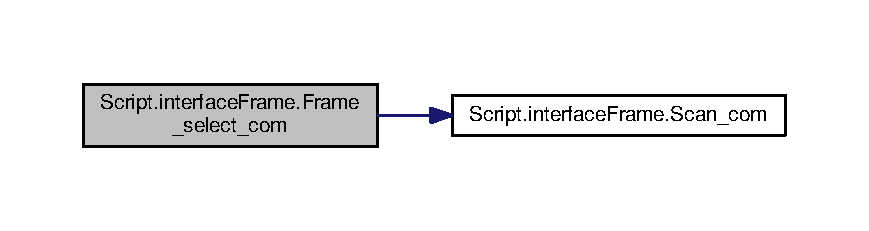
\includegraphics[width=350pt]{namespaceScript_1_1interfaceFrame_a3538cb8357b74776a380240ed3221bc0_cgraph}
\end{center}
\end{figure}
\mbox{\Hypertarget{namespaceScript_1_1interfaceFrame_a76119121c3aceb43846ba3ea526623ad}\label{namespaceScript_1_1interfaceFrame_a76119121c3aceb43846ba3ea526623ad}} 
\index{Script\+::interface\+Frame@{Script\+::interface\+Frame}!Scan\+\_\+com@{Scan\+\_\+com}}
\index{Scan\+\_\+com@{Scan\+\_\+com}!Script\+::interface\+Frame@{Script\+::interface\+Frame}}
\subsubsection{\texorpdfstring{Scan\+\_\+com()}{Scan\_com()}}
{\footnotesize\ttfamily def Script.\+interface\+Frame.\+Scan\+\_\+com (\begin{DoxyParamCaption}{ }\end{DoxyParamCaption})}



Définition à la ligne 317 du fichier interface\+Frame.\+py.



Référencé par Script.\+interface\+Frame.\+Frame\+\_\+select\+\_\+com().


\begin{DoxyCode}
317 \textcolor{keyword}{def }\hyperlink{namespaceScript_1_1interfaceFrame_a76119121c3aceb43846ba3ea526623ad}{Scan\_com}():
318     available=[]
319     \textcolor{keywordflow}{try}:
320         \textcolor{keywordflow}{for} i \textcolor{keywordflow}{in} range(256):
321             \textcolor{keywordflow}{try}:
322                 ser = serial.Serial(i)
323                 available.append(str(ser.portstr))
324                 ser.close
325             \textcolor{keywordflow}{except} serial.SerialException:
326                 \textcolor{keywordflow}{pass}
327         \textcolor{keywordflow}{return} available
328     \textcolor{keywordflow}{except} Exception \textcolor{keyword}{as} e:
329         print(\textcolor{stringliteral}{"In file Interface; ligne 247"})
330         print(e)
331 
332 \textcolor{comment}{# cette Fonction verifie que tous les arguments
}
333 \textcolor{comment}{# elle verifie que tous les information nécessaire sont siasie 
}
334 \textcolor{comment}{# cela permet d'eviter des bugs ou errors
}
\end{DoxyCode}
Voici le graphe des appelants de cette fonction \+:\nopagebreak
\begin{figure}[H]
\begin{center}
\leavevmode
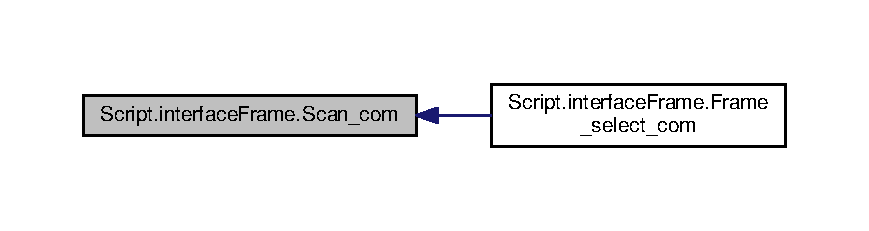
\includegraphics[width=350pt]{namespaceScript_1_1interfaceFrame_a76119121c3aceb43846ba3ea526623ad_icgraph}
\end{center}
\end{figure}
\mbox{\Hypertarget{namespaceScript_1_1interfaceFrame_ab554e77db5080fb2eae78e39ebbeb395}\label{namespaceScript_1_1interfaceFrame_ab554e77db5080fb2eae78e39ebbeb395}} 
\index{Script\+::interface\+Frame@{Script\+::interface\+Frame}!split\+\_\+chaine@{split\+\_\+chaine}}
\index{split\+\_\+chaine@{split\+\_\+chaine}!Script\+::interface\+Frame@{Script\+::interface\+Frame}}
\subsubsection{\texorpdfstring{split\+\_\+chaine()}{split\_chaine()}}
{\footnotesize\ttfamily def Script.\+interface\+Frame.\+split\+\_\+chaine (\begin{DoxyParamCaption}\item[{}]{chaine,  }\item[{}]{caractere }\end{DoxyParamCaption})}



Définition à la ligne 429 du fichier interface\+Frame.\+py.


\begin{DoxyCode}
429 \textcolor{keyword}{def }\hyperlink{namespaceScript_1_1interfaceFrame_ab554e77db5080fb2eae78e39ebbeb395}{split\_chaine}(chaine, caractere):
430     carac\_chaine=[\textcolor{stringliteral}{"["},\textcolor{stringliteral}{"]"}, \textcolor{stringliteral}{"\(\backslash\)n"}, \textcolor{stringliteral}{"\(\backslash\)r"}]
431     new\_chaine=\textcolor{stringliteral}{""}
432     \textcolor{keywordflow}{try}:
433         \textcolor{keywordflow}{for} line \textcolor{keywordflow}{in} chaine:
434             i=0
435             \textcolor{keywordflow}{while} i < len(line):
436                 \textcolor{keywordflow}{if} line[i] \textcolor{keywordflow}{not} \textcolor{keywordflow}{in} carac\_chaine:
437                     new\_chaine=new\_chaine+line[i]
438                 i+=1
439             \textcolor{stringliteral}{"""
}
440 \textcolor{stringliteral}{            adding character tosepare the elements of the character string
}
441 \textcolor{stringliteral}{            """}
442             new\_chaine+=caractere
443 
444         \textcolor{keywordflow}{return} new\_chaine
445     \textcolor{keywordflow}{except} Exception \textcolor{keyword}{as} e:
446         print(\textcolor{stringliteral}{"In file Interface; ligne 346"})
447         print(e)
448         \textcolor{keywordflow}{return} \textcolor{keywordtype}{None} 
449 \end{DoxyCode}
\mbox{\Hypertarget{namespaceScript_1_1interfaceFrame_a7a90dd83e0b67edcf2dee870d927e98e}\label{namespaceScript_1_1interfaceFrame_a7a90dd83e0b67edcf2dee870d927e98e}} 
\index{Script\+::interface\+Frame@{Script\+::interface\+Frame}!verif\+\_\+args@{verif\+\_\+args}}
\index{verif\+\_\+args@{verif\+\_\+args}!Script\+::interface\+Frame@{Script\+::interface\+Frame}}
\subsubsection{\texorpdfstring{verif\+\_\+args()}{verif\_args()}}
{\footnotesize\ttfamily def Script.\+interface\+Frame.\+verif\+\_\+args (\begin{DoxyParamCaption}{ }\end{DoxyParamCaption})}



Définition à la ligne 335 du fichier interface\+Frame.\+py.



Référencé par Script.\+interface\+Frame.\+Frame\+\_\+btn\+\_\+execution().


\begin{DoxyCode}
335 \textcolor{keyword}{def }\hyperlink{namespaceScript_1_1interfaceFrame_a7a90dd83e0b67edcf2dee870d927e98e}{verif\_args}():
336     \textcolor{keyword}{global} VALUE\_BOX\_COM1 
337     \textcolor{keyword}{global} VALUE\_BOX\_COM2
338     
339     \textcolor{keyword}{global} VALUE\_SELECT\_CALL\_OPTION
340     \textcolor{keyword}{global} VALUE\_SELECT\_CALL\_CONFIG
341     
342     \textcolor{keyword}{global} VALUE\_ENTRY\_PHONE\_NUMERO
343     \textcolor{keyword}{global} VALUE\_ENTRY\_ATCBST
344 
345     \textcolor{keyword}{global} VALUE\_ENTRY\_OMC\_IP
346     \textcolor{keyword}{global} VALUE\_ENTRY\_OMC\_PASSWORD
347     \textcolor{keyword}{global} VALUE\_ENTRY\_OMC\_USER
348 
349     \textcolor{keyword}{global} VALUE\_ENTRY\_OMU1\_IP
350     \textcolor{keyword}{global} VALUE\_ENTRY\_OMU1\_PASSWORD
351     \textcolor{keyword}{global} VALUE\_ENTRY\_OMU1\_USER
352 
353     \textcolor{keyword}{global} VALUE\_ENTRY\_OMU2\_IP
354     \textcolor{keyword}{global} VALUE\_ENTRY\_OMU2\_PASSWORD
355     \textcolor{keyword}{global} VALUE\_ENTRY\_OMU2\_USER
356 
357     msg\_error= 1
358 
359     tmu\_mode= \textcolor{keyword}{False}
360     simple\_mode= \textcolor{keyword}{False}
361     ptp\_mode= \textcolor{keyword}{False}
362     data\_mode= \textcolor{keyword}{False}
363     vgcs\_mode= \textcolor{keyword}{False}
364     rec\_mode= \textcolor{keyword}{False}
365     vbs\_mode= \textcolor{keyword}{False}
366 
367     \textcolor{comment}{# On veirifie que les entrés sont bien présent
}
368     \textcolor{comment}{# On verifie l'existance des tous les chanmps obligatoire
}
369     \textcolor{comment}{# ensuite on essaye de savoir les options utilisé par l'utilisateur
}
370     \textcolor{keywordflow}{if} (len(VALUE\_ENTRY\_OMC\_IP.get()) > 0) \textcolor{keywordflow}{and} (len(VALUE\_ENTRY\_OMC\_USER.get()) > 0) \textcolor{keywordflow}{and} (len(
      VALUE\_ENTRY\_OMC\_PASSWORD.get()) > 0) \textcolor{keywordflow}{and}\(\backslash\)
371     (len(VALUE\_ENTRY\_OMU1\_IP.get()) > 0) \textcolor{keywordflow}{and} (len(VALUE\_ENTRY\_OMU1\_USER.get()) > 0) \textcolor{keywordflow}{and} (len(
      VALUE\_ENTRY\_OMU1\_PASSWORD.get()) > 0) \textcolor{keywordflow}{and} \(\backslash\)
372     (len(VALUE\_ENTRY\_OMU2\_IP.get()) > 0) \textcolor{keywordflow}{and} (len(VALUE\_ENTRY\_OMU2\_USER.get()) > 0) \textcolor{keywordflow}{and} (len(
      VALUE\_ENTRY\_OMU2\_PASSWORD.get()) > 0) \textcolor{keywordflow}{and} \(\backslash\)
373     (len(VALUE\_BOX\_COM1.get()) > 0) \textcolor{keywordflow}{and} (VALUE\_BOX\_COM1.get()  != VALUE\_BOX\_COM2.get()) \textcolor{keywordflow}{and} (len(
      VALUE\_ENTRY\_PHONE\_NUMERO.get()) > 0) \textcolor{keywordflow}{and} \(\backslash\)
374     (len(VALUE\_ENTRY\_GROUP\_ID.get()) > 0) \textcolor{keywordflow}{and} (len(VALUE\_ENTRY\_ATCBST.get()) > 0) \textcolor{keywordflow}{and} (len(
      VALUE\_ENTRY\_NB\_RTMU.get()) > 0):
375         
376         \textcolor{comment}{# lacette Boucle permet de savoir la configuration choisi par l'utilisateur
}
377         \textcolor{comment}{# On  deux type de configuration SIMPLe pour un handOver simple ou RESET-TMU pour reseter le TMU
}
378         \textcolor{keywordflow}{for} cle \textcolor{keywordflow}{in} VALUE\_SELECT\_CALL\_CONFIG:
379             \textcolor{keywordflow}{if} VALUE\_SELECT\_CALL\_CONFIG[cle].get() == 1:
380                 \textcolor{keywordflow}{if} cle == \textcolor{stringliteral}{"SIMPLE"}:
381                     simple\_mode= \textcolor{keyword}{True}
382                     set\_config= \textcolor{keyword}{True}
383                 \textcolor{keywordflow}{elif} cle == \textcolor{stringliteral}{"RESET-TMU"}:
384                     tmu\_mode= \textcolor{keyword}{True}
385                     set\_config= \textcolor{keyword}{True}
386                 \textcolor{keywordflow}{else}:
387                     set\_config= \textcolor{keyword}{False}
388                     print(\textcolor{stringliteral}{"Veuillez remplir tous les champs"})
389 
390         \textcolor{comment}{# Ici chercher à savoir les types d'appel choisi par l'utilisateur
}
391         \textcolor{comment}{# ce types peut PTP pour l'appel voix
}
392         \textcolor{comment}{# DATA pour appel data
}
393         \textcolor{comment}{# VGCS VBS et REC font parties de la famille de groupe call ensuite on fait appel a la classe
       handOver pour en lui donnant les paramètre
}
394         \textcolor{keywordflow}{for} cle \textcolor{keywordflow}{in} VALUE\_SELECT\_CALL\_OPTION:
395             \textcolor{keywordflow}{if} VALUE\_SELECT\_CALL\_OPTION[cle].get() == 1:
396                 \textcolor{keywordflow}{if} cle == \textcolor{stringliteral}{"PTP"}:
397                     ptp\_mode= \textcolor{keyword}{True}
398                     set\_call\_option= \textcolor{keyword}{True}
399                 \textcolor{keywordflow}{elif} cle == \textcolor{stringliteral}{"DATA"}:
400                     data\_mode = \textcolor{keyword}{True}
401                     set\_call\_option= \textcolor{keyword}{True}
402                 \textcolor{keywordflow}{elif} cle == \textcolor{stringliteral}{"VGCS"}:
403                     vgcs\_mode= \textcolor{keyword}{True}
404                     set\_call\_option= \textcolor{keyword}{True}
405                 \textcolor{keywordflow}{elif} cle == \textcolor{stringliteral}{"REC"}:
406                     rec\_mode= \textcolor{keyword}{True}
407                     set\_call\_option= \textcolor{keyword}{True}
408                 \textcolor{keywordflow}{elif} cle == \textcolor{stringliteral}{"VBS"}:
409                     vbs\_mode= \textcolor{keyword}{True}
410                     set\_call\_option= \textcolor{keyword}{True}
411                 \textcolor{keywordflow}{else}:
412                     set\_call\_option= \textcolor{keyword}{False}
413                     print(\textcolor{stringliteral}{"Veuillez remplir tous les champs"})
414         
415         \textcolor{keywordflow}{if} (set\_call\_option== \textcolor{keyword}{False}) \textcolor{keywordflow}{or} (set\_config== \textcolor{keyword}{False}):
416             print(\textcolor{stringliteral}{"Veuillez remplir tous les champs"})
417         \textcolor{keywordflow}{else}:
418             \textcolor{comment}{# On fait appel de la classe begin\_handOver une fois que l'utilisateur clic sur le bouton
       d'exécuter
}
419             handOver.begin\_handOver(simple\_mode, tmu\_mode, ptp\_mode, data\_mode, vgcs\_mode, rec\_mode, 
      vbs\_mode)
420     \textcolor{keywordflow}{else}:
421         print(\textcolor{stringliteral}{"Veuillez remplir tous les champs"})
422 
423 
424 
425 \textcolor{comment}{# Cette fonction de supprimer des caractère speciaux lorqu'on fait un read du mobile
}
426 \textcolor{comment}{# Cela permet de mieux veirifier que les information retourner par le mobile
}
427 \textcolor{comment}{# Ca aide le programme à mieux prendre les decision 
}
428 
\end{DoxyCode}
Voici le graphe des appelants de cette fonction \+:\nopagebreak
\begin{figure}[H]
\begin{center}
\leavevmode
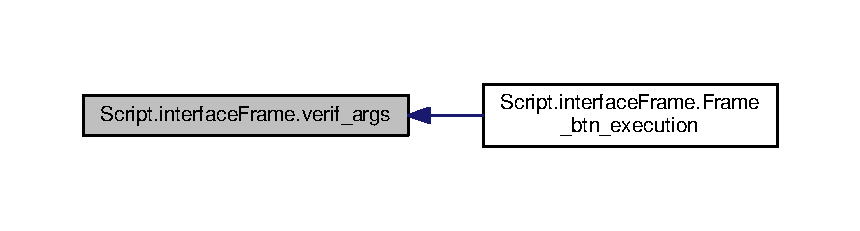
\includegraphics[width=350pt]{namespaceScript_1_1interfaceFrame_a7a90dd83e0b67edcf2dee870d927e98e_icgraph}
\end{center}
\end{figure}


\subsection{Documentation des variables}
\mbox{\Hypertarget{namespaceScript_1_1interfaceFrame_ab8e385a4d6a1f87628b963bc0a385519}\label{namespaceScript_1_1interfaceFrame_ab8e385a4d6a1f87628b963bc0a385519}} 
\index{Script\+::interface\+Frame@{Script\+::interface\+Frame}!begin\+\_\+time@{begin\+\_\+time}}
\index{begin\+\_\+time@{begin\+\_\+time}!Script\+::interface\+Frame@{Script\+::interface\+Frame}}
\subsubsection{\texorpdfstring{begin\+\_\+time}{begin\_time}}
{\footnotesize\ttfamily Script.\+interface\+Frame.\+begin\+\_\+time = time.\+time()}



Définition à la ligne 43 du fichier interface\+Frame.\+py.

\mbox{\Hypertarget{namespaceScript_1_1interfaceFrame_ace1207561541cc3ee3af9b2f33b2a316}\label{namespaceScript_1_1interfaceFrame_ace1207561541cc3ee3af9b2f33b2a316}} 
\index{Script\+::interface\+Frame@{Script\+::interface\+Frame}!val\+\_\+line@{val\+\_\+line}}
\index{val\+\_\+line@{val\+\_\+line}!Script\+::interface\+Frame@{Script\+::interface\+Frame}}
\subsubsection{\texorpdfstring{val\+\_\+line}{val\_line}}
{\footnotesize\ttfamily int Script.\+interface\+Frame.\+val\+\_\+line = 0}



Définition à la ligne 45 du fichier interface\+Frame.\+py.

\mbox{\Hypertarget{namespaceScript_1_1interfaceFrame_a235ac21d18cefa672100db29db0ed490}\label{namespaceScript_1_1interfaceFrame_a235ac21d18cefa672100db29db0ed490}} 
\index{Script\+::interface\+Frame@{Script\+::interface\+Frame}!V\+A\+L\+U\+E\+\_\+\+F\+I\+L\+E\+\_\+\+A\+U\+D\+IO@{V\+A\+L\+U\+E\+\_\+\+F\+I\+L\+E\+\_\+\+A\+U\+D\+IO}}
\index{V\+A\+L\+U\+E\+\_\+\+F\+I\+L\+E\+\_\+\+A\+U\+D\+IO@{V\+A\+L\+U\+E\+\_\+\+F\+I\+L\+E\+\_\+\+A\+U\+D\+IO}!Script\+::interface\+Frame@{Script\+::interface\+Frame}}
\subsubsection{\texorpdfstring{V\+A\+L\+U\+E\+\_\+\+F\+I\+L\+E\+\_\+\+A\+U\+D\+IO}{VALUE\_FILE\_AUDIO}}
{\footnotesize\ttfamily string Script.\+interface\+Frame.\+V\+A\+L\+U\+E\+\_\+\+F\+I\+L\+E\+\_\+\+A\+U\+D\+IO = \char`\"{}\char`\"{}}



Définition à la ligne 49 du fichier interface\+Frame.\+py.

\mbox{\Hypertarget{namespaceScript_1_1interfaceFrame_a3704b57444e587c904b839d2dfef2b7e}\label{namespaceScript_1_1interfaceFrame_a3704b57444e587c904b839d2dfef2b7e}} 
\index{Script\+::interface\+Frame@{Script\+::interface\+Frame}!V\+A\+L\+U\+E\+\_\+\+F\+I\+L\+E\+\_\+\+C\+MD@{V\+A\+L\+U\+E\+\_\+\+F\+I\+L\+E\+\_\+\+C\+MD}}
\index{V\+A\+L\+U\+E\+\_\+\+F\+I\+L\+E\+\_\+\+C\+MD@{V\+A\+L\+U\+E\+\_\+\+F\+I\+L\+E\+\_\+\+C\+MD}!Script\+::interface\+Frame@{Script\+::interface\+Frame}}
\subsubsection{\texorpdfstring{V\+A\+L\+U\+E\+\_\+\+F\+I\+L\+E\+\_\+\+C\+MD}{VALUE\_FILE\_CMD}}
{\footnotesize\ttfamily string Script.\+interface\+Frame.\+V\+A\+L\+U\+E\+\_\+\+F\+I\+L\+E\+\_\+\+C\+MD = \char`\"{}\char`\"{}}



Définition à la ligne 47 du fichier interface\+Frame.\+py.

\mbox{\Hypertarget{namespaceScript_1_1interfaceFrame_a2cfacdb24b52e8cf5d9667d91a5c58ab}\label{namespaceScript_1_1interfaceFrame_a2cfacdb24b52e8cf5d9667d91a5c58ab}} 
\index{Script\+::interface\+Frame@{Script\+::interface\+Frame}!V\+A\+L\+U\+E\+\_\+\+F\+I\+L\+E\+\_\+\+C\+O\+NF@{V\+A\+L\+U\+E\+\_\+\+F\+I\+L\+E\+\_\+\+C\+O\+NF}}
\index{V\+A\+L\+U\+E\+\_\+\+F\+I\+L\+E\+\_\+\+C\+O\+NF@{V\+A\+L\+U\+E\+\_\+\+F\+I\+L\+E\+\_\+\+C\+O\+NF}!Script\+::interface\+Frame@{Script\+::interface\+Frame}}
\subsubsection{\texorpdfstring{V\+A\+L\+U\+E\+\_\+\+F\+I\+L\+E\+\_\+\+C\+O\+NF}{VALUE\_FILE\_CONF}}
{\footnotesize\ttfamily string Script.\+interface\+Frame.\+V\+A\+L\+U\+E\+\_\+\+F\+I\+L\+E\+\_\+\+C\+O\+NF = \char`\"{}\char`\"{}}



Définition à la ligne 46 du fichier interface\+Frame.\+py.

\mbox{\Hypertarget{namespaceScript_1_1interfaceFrame_a8933d662775f7e5fc3e0b8e5fb499b24}\label{namespaceScript_1_1interfaceFrame_a8933d662775f7e5fc3e0b8e5fb499b24}} 
\index{Script\+::interface\+Frame@{Script\+::interface\+Frame}!V\+A\+L\+U\+E\+\_\+\+F\+I\+L\+E\+\_\+\+S\+A\+VE@{V\+A\+L\+U\+E\+\_\+\+F\+I\+L\+E\+\_\+\+S\+A\+VE}}
\index{V\+A\+L\+U\+E\+\_\+\+F\+I\+L\+E\+\_\+\+S\+A\+VE@{V\+A\+L\+U\+E\+\_\+\+F\+I\+L\+E\+\_\+\+S\+A\+VE}!Script\+::interface\+Frame@{Script\+::interface\+Frame}}
\subsubsection{\texorpdfstring{V\+A\+L\+U\+E\+\_\+\+F\+I\+L\+E\+\_\+\+S\+A\+VE}{VALUE\_FILE\_SAVE}}
{\footnotesize\ttfamily string Script.\+interface\+Frame.\+V\+A\+L\+U\+E\+\_\+\+F\+I\+L\+E\+\_\+\+S\+A\+VE = \char`\"{}\char`\"{}}



Définition à la ligne 48 du fichier interface\+Frame.\+py.


\hypertarget{namespaceScript_1_1omc}{}\section{Référence de l\textquotesingle{}espace de nommage Script.\+omc}
\label{namespaceScript_1_1omc}\index{Script.\+omc@{Script.\+omc}}
\subsection*{Classes}
\begin{DoxyCompactItemize}
\item 
class \hyperlink{classScript_1_1omc_1_1OMC}{O\+MC}
\end{DoxyCompactItemize}

\hypertarget{namespaceScript_1_1omu}{}\section{Référence de l\textquotesingle{}espace de nommage Script.\+omu}
\label{namespaceScript_1_1omu}\index{Script.\+omu@{Script.\+omu}}
\subsection*{Classes}
\begin{DoxyCompactItemize}
\item 
class \hyperlink{classScript_1_1omu_1_1OMU}{O\+MU}
\end{DoxyCompactItemize}

\hypertarget{namespaceScript_1_1Option}{}\section{Référence de l\textquotesingle{}espace de nommage Script.\+Option}
\label{namespaceScript_1_1Option}\index{Script.\+Option@{Script.\+Option}}
\subsection*{Fonctions}
\begin{DoxyCompactItemize}
\item 
def \hyperlink{namespaceScript_1_1Option_abb674ebac6565861fc8240a9306f8ecd}{callback\+\_\+quit} ()
\item 
def \hyperlink{namespaceScript_1_1Option_aff91639f98fde0463987ea08e565da05}{progress\+\_\+\+Bar} ()
\item 
def \hyperlink{namespaceScript_1_1Option_a09506d9cf0343fc80883c5db0a207737}{save\+\_\+\+Data} (my\+\_\+object)
\item 
def \hyperlink{namespaceScript_1_1Option_ac71533bc42f23543f3c564ccf01d9faf}{split\+\_\+chaine} (chaine, caractere)
\item 
def \hyperlink{namespaceScript_1_1Option_a1707d1e8b288159100845df330fc8d51}{limit\+\_\+waiting} ()
\item 
def \hyperlink{namespaceScript_1_1Option_a22c03fd81ddb28ef13f194565b4996ba}{hang\+\_\+up\+\_\+call} (phone)
\end{DoxyCompactItemize}


\subsection{Documentation des fonctions}
\mbox{\Hypertarget{namespaceScript_1_1Option_abb674ebac6565861fc8240a9306f8ecd}\label{namespaceScript_1_1Option_abb674ebac6565861fc8240a9306f8ecd}} 
\index{Script\+::\+Option@{Script\+::\+Option}!callback\+\_\+quit@{callback\+\_\+quit}}
\index{callback\+\_\+quit@{callback\+\_\+quit}!Script\+::\+Option@{Script\+::\+Option}}
\subsubsection{\texorpdfstring{callback\+\_\+quit()}{callback\_quit()}}
{\footnotesize\ttfamily def Script.\+Option.\+callback\+\_\+quit (\begin{DoxyParamCaption}{ }\end{DoxyParamCaption})}



Définition à la ligne 20 du fichier Option.\+py.



Référencé par Script.\+Option.\+progress\+\_\+\+Bar().


\begin{DoxyCode}
20 \textcolor{keyword}{def }\hyperlink{namespaceScript_1_1Option_abb674ebac6565861fc8240a9306f8ecd}{callback\_quit}():
21     \textcolor{keyword}{global} RUNNING
22     \textcolor{keywordflow}{if} tkMessageBox.askokcancel(\textcolor{stringliteral}{"Quitter"}, \textcolor{stringliteral}{"êtes-vous sûr de vouloir quitter?"}):
23         toplevel.destroy()
24         RUNNING= \textcolor{keyword}{False}
25 
26 \textcolor{stringliteral}{"""
}
27 \textcolor{stringliteral}{Comme son indique progress\_Bar est une barre de progression en mode de dure indertiminé. 
}
28 \textcolor{stringliteral}{Elle s'execute au premier plan et masqué la fenetre principale pour empêcher toute motidification possible
}
29 \textcolor{stringliteral}{"""}
\end{DoxyCode}
Voici le graphe des appelants de cette fonction \+:\nopagebreak
\begin{figure}[H]
\begin{center}
\leavevmode
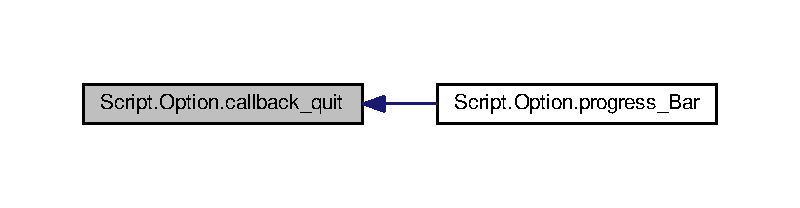
\includegraphics[width=350pt]{namespaceScript_1_1Option_abb674ebac6565861fc8240a9306f8ecd_icgraph}
\end{center}
\end{figure}
\mbox{\Hypertarget{namespaceScript_1_1Option_a22c03fd81ddb28ef13f194565b4996ba}\label{namespaceScript_1_1Option_a22c03fd81ddb28ef13f194565b4996ba}} 
\index{Script\+::\+Option@{Script\+::\+Option}!hang\+\_\+up\+\_\+call@{hang\+\_\+up\+\_\+call}}
\index{hang\+\_\+up\+\_\+call@{hang\+\_\+up\+\_\+call}!Script\+::\+Option@{Script\+::\+Option}}
\subsubsection{\texorpdfstring{hang\+\_\+up\+\_\+call()}{hang\_up\_call()}}
{\footnotesize\ttfamily def Script.\+Option.\+hang\+\_\+up\+\_\+call (\begin{DoxyParamCaption}\item[{}]{phone }\end{DoxyParamCaption})}



Définition à la ligne 106 du fichier Option.\+py.



Référencé par Script.\+Option.\+limit\+\_\+waiting().


\begin{DoxyCode}
106 \textcolor{keyword}{def }\hyperlink{namespaceScript_1_1Option_a22c03fd81ddb28ef13f194565b4996ba}{hang\_up\_call}(phone):
107     \textcolor{comment}{#phone.write("\(\backslash\)r")
}
108     time.sleep(1)
109     phone.write(b\textcolor{stringliteral}{"+"})
110     phone.write(b\textcolor{stringliteral}{"+"})
111     phone.write(b\textcolor{stringliteral}{"+"})
112     time.sleep(2)
113     phone.write(\textcolor{stringliteral}{"\(\backslash\)r"})
114     time.sleep(2)
115     phone.write(b\textcolor{stringliteral}{"ath\(\backslash\)r"})
116     time.sleep(3)
117     print(\textcolor{stringliteral}{"++ath"})
118     phone.readlines()
119 \end{DoxyCode}
Voici le graphe des appelants de cette fonction \+:\nopagebreak
\begin{figure}[H]
\begin{center}
\leavevmode
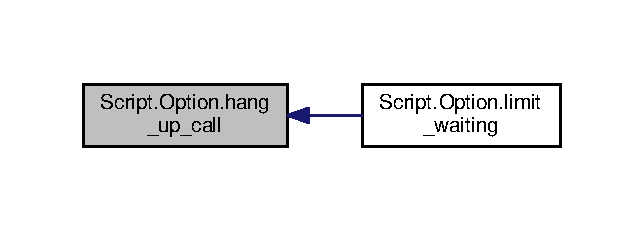
\includegraphics[width=309pt]{namespaceScript_1_1Option_a22c03fd81ddb28ef13f194565b4996ba_icgraph}
\end{center}
\end{figure}
\mbox{\Hypertarget{namespaceScript_1_1Option_a1707d1e8b288159100845df330fc8d51}\label{namespaceScript_1_1Option_a1707d1e8b288159100845df330fc8d51}} 
\index{Script\+::\+Option@{Script\+::\+Option}!limit\+\_\+waiting@{limit\+\_\+waiting}}
\index{limit\+\_\+waiting@{limit\+\_\+waiting}!Script\+::\+Option@{Script\+::\+Option}}
\subsubsection{\texorpdfstring{limit\+\_\+waiting()}{limit\_waiting()}}
{\footnotesize\ttfamily def Script.\+Option.\+limit\+\_\+waiting (\begin{DoxyParamCaption}{ }\end{DoxyParamCaption})}



Définition à la ligne 83 du fichier Option.\+py.



Références Script.\+Option.\+hang\+\_\+up\+\_\+call().


\begin{DoxyCode}
83 \textcolor{keyword}{def }\hyperlink{namespaceScript_1_1Option_a1707d1e8b288159100845df330fc8d51}{limit\_waiting}():
84     \textcolor{keyword}{global} RUNNING
85     \textcolor{keyword}{global} signal\_limit\_waiting
86     \textcolor{keyword}{global} val\_continue
87     \textcolor{keyword}{global} phone\_com1
88     \textcolor{keyword}{global} val\_stage
89 
90     signal\_limit\_waiting= \textcolor{keyword}{False}
91     val\_stage= 0
92 
93     \textcolor{keywordflow}{while} RUNNING == \textcolor{keyword}{True}:
94         \textcolor{keywordflow}{if} signal\_limit\_waiting == \textcolor{keyword}{True}:
95             stage= val\_stage
96             val\_continue= \textcolor{keyword}{True}
97             time.sleep(90)
98             \textcolor{keywordflow}{if} val\_continue == \textcolor{keyword}{True} \textcolor{keywordflow}{and} stage== val\_stage:
99                 \hyperlink{namespaceScript_1_1Option_a22c03fd81ddb28ef13f194565b4996ba}{hang\_up\_call}(phone\_com1)
100 
101 
102 
103 \textcolor{stringliteral}{"""
}
104 \textcolor{stringliteral}{hang\_up\_call est la fonction qui permet de racrocher un appel DATA
}
105 \textcolor{stringliteral}{"""}
\end{DoxyCode}
Voici le graphe d\textquotesingle{}appel pour cette fonction \+:\nopagebreak
\begin{figure}[H]
\begin{center}
\leavevmode
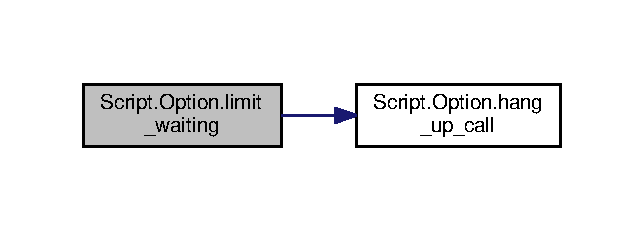
\includegraphics[width=309pt]{namespaceScript_1_1Option_a1707d1e8b288159100845df330fc8d51_cgraph}
\end{center}
\end{figure}
\mbox{\Hypertarget{namespaceScript_1_1Option_aff91639f98fde0463987ea08e565da05}\label{namespaceScript_1_1Option_aff91639f98fde0463987ea08e565da05}} 
\index{Script\+::\+Option@{Script\+::\+Option}!progress\+\_\+\+Bar@{progress\+\_\+\+Bar}}
\index{progress\+\_\+\+Bar@{progress\+\_\+\+Bar}!Script\+::\+Option@{Script\+::\+Option}}
\subsubsection{\texorpdfstring{progress\+\_\+\+Bar()}{progress\_Bar()}}
{\footnotesize\ttfamily def Script.\+Option.\+progress\+\_\+\+Bar (\begin{DoxyParamCaption}{ }\end{DoxyParamCaption})}



Définition à la ligne 30 du fichier Option.\+py.



Références Script.\+Option.\+callback\+\_\+quit().


\begin{DoxyCode}
30 \textcolor{keyword}{def }\hyperlink{namespaceScript_1_1Option_aff91639f98fde0463987ea08e565da05}{progress\_Bar}():
31     \textcolor{keyword}{global} RUNNING
32     \textcolor{keyword}{global} toplevel
33     \textcolor{keywordflow}{try}:
34         RUNNING= \textcolor{keyword}{True}
35         toplevel= Toplevel()
36         toplevel.progress = ttk.Progressbar(toplevel, orient=\textcolor{stringliteral}{"horizontal"},length=380, mode=\textcolor{stringliteral}{"indeterminate"})
      
37         toplevel.progress.pack()
38         thread = threading.Thread()
39         thread.\_\_init\_\_(target=toplevel.progress.start(), args=())
40         thread.start
41         toplevel.grab\_set()
42         toplevel.focus\_set()
43         toplevel.focus\_force
44 
45         \textcolor{stringliteral}{"""
}
46 \textcolor{stringliteral}{        On detecte si l'utisateur clic sur le bouton fermer,
}
47 \textcolor{stringliteral}{        alors on appelle la fonction callback\_quit pour confirmer le choix 
}
48 \textcolor{stringliteral}{        """}
49         toplevel.protocol(\textcolor{stringliteral}{"WM\_DELETE\_WINDOW"}, \textcolor{keyword}{lambda}:\hyperlink{namespaceScript_1_1Option_abb674ebac6565861fc8240a9306f8ecd}{callback\_quit}())
50     \textcolor{keywordflow}{except} Exception \textcolor{keyword}{as} e:
51         print(\textcolor{stringliteral}{"in file Option, progressbar"})
52         print(e)
53         RUNNING = \textcolor{keyword}{False}
54     
55 
56 
57 \textcolor{stringliteral}{"""
}
58 \textcolor{stringliteral}{La fonction permet d'enregistre les donneés dans le fichier de rapport choisi par l'utilisateur 
}
59 \textcolor{stringliteral}{elle est utilisé dans le cas si l'utilisateur choisi l'option NR\_DATA
}
60 \textcolor{stringliteral}{"""}
\end{DoxyCode}
Voici le graphe d\textquotesingle{}appel pour cette fonction \+:\nopagebreak
\begin{figure}[H]
\begin{center}
\leavevmode
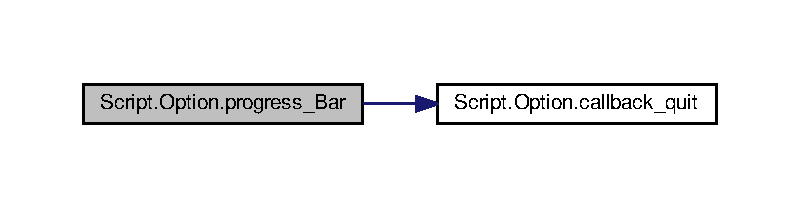
\includegraphics[width=350pt]{namespaceScript_1_1Option_aff91639f98fde0463987ea08e565da05_cgraph}
\end{center}
\end{figure}
\mbox{\Hypertarget{namespaceScript_1_1Option_a09506d9cf0343fc80883c5db0a207737}\label{namespaceScript_1_1Option_a09506d9cf0343fc80883c5db0a207737}} 
\index{Script\+::\+Option@{Script\+::\+Option}!save\+\_\+\+Data@{save\+\_\+\+Data}}
\index{save\+\_\+\+Data@{save\+\_\+\+Data}!Script\+::\+Option@{Script\+::\+Option}}
\subsubsection{\texorpdfstring{save\+\_\+\+Data()}{save\_Data()}}
{\footnotesize\ttfamily def Script.\+Option.\+save\+\_\+\+Data (\begin{DoxyParamCaption}\item[{}]{my\+\_\+object }\end{DoxyParamCaption})}



Définition à la ligne 61 du fichier Option.\+py.


\begin{DoxyCode}
61 \textcolor{keyword}{def }\hyperlink{namespaceScript_1_1Option_a09506d9cf0343fc80883c5db0a207737}{save\_Data}(my\_object):
62     with open(interfaceFrame.VALUE\_FILE\_SAVE, \textcolor{stringliteral}{"a"}) \textcolor{keyword}{as} fichier:  
63         fichier.write(my\_object)
64         fichier.closed
65 
66 \textcolor{stringliteral}{"""
}
67 \textcolor{stringliteral}{elle convertit la liste chaine en string et ajoute caractere a chaque tour de la boucle
}
68 \textcolor{stringliteral}{"""}
\end{DoxyCode}
\mbox{\Hypertarget{namespaceScript_1_1Option_ac71533bc42f23543f3c564ccf01d9faf}\label{namespaceScript_1_1Option_ac71533bc42f23543f3c564ccf01d9faf}} 
\index{Script\+::\+Option@{Script\+::\+Option}!split\+\_\+chaine@{split\+\_\+chaine}}
\index{split\+\_\+chaine@{split\+\_\+chaine}!Script\+::\+Option@{Script\+::\+Option}}
\subsubsection{\texorpdfstring{split\+\_\+chaine()}{split\_chaine()}}
{\footnotesize\ttfamily def Script.\+Option.\+split\+\_\+chaine (\begin{DoxyParamCaption}\item[{}]{chaine,  }\item[{}]{caractere }\end{DoxyParamCaption})}



Définition à la ligne 69 du fichier Option.\+py.


\begin{DoxyCode}
69 \textcolor{keyword}{def }\hyperlink{namespaceScript_1_1Option_ac71533bc42f23543f3c564ccf01d9faf}{split\_chaine}(chaine, caractere):
70     carac\_chaine=[\textcolor{stringliteral}{"["},\textcolor{stringliteral}{"]"}, \textcolor{stringliteral}{"\(\backslash\)n"}, \textcolor{stringliteral}{"\(\backslash\)r"}]
71     new\_chaine=\textcolor{stringliteral}{""}
72     \textcolor{keywordflow}{for} line \textcolor{keywordflow}{in} chaine:
73         i=0
74         \textcolor{keywordflow}{while} i < len(line):
75             \textcolor{keywordflow}{if} line[i] \textcolor{keywordflow}{not} \textcolor{keywordflow}{in} carac\_chaine:
76                 new\_chaine=new\_chaine+line[i]
77             i+=1
78         new\_chaine+=caractere
79 
80     \textcolor{keywordflow}{return} new\_chaine
81 
82 
\end{DoxyCode}

\hypertarget{namespaceScript_1_1progress__bar}{}\section{Référence de l\textquotesingle{}espace de nommage Script.\+progress\+\_\+bar}
\label{namespaceScript_1_1progress__bar}\index{Script.\+progress\+\_\+bar@{Script.\+progress\+\_\+bar}}
\subsection*{Classes}
\begin{DoxyCompactItemize}
\item 
class \hyperlink{classScript_1_1progress__bar_1_1SampleApp}{Sample\+App}
\end{DoxyCompactItemize}
\subsection*{Variables}
\begin{DoxyCompactItemize}
\item 
\hyperlink{namespaceScript_1_1progress__bar_a2346ccb846bab632249778f76d43e342}{app} = \hyperlink{classScript_1_1progress__bar_1_1SampleApp}{Sample\+App}()
\end{DoxyCompactItemize}


\subsection{Documentation des variables}
\mbox{\Hypertarget{namespaceScript_1_1progress__bar_a2346ccb846bab632249778f76d43e342}\label{namespaceScript_1_1progress__bar_a2346ccb846bab632249778f76d43e342}} 
\index{Script\+::progress\+\_\+bar@{Script\+::progress\+\_\+bar}!app@{app}}
\index{app@{app}!Script\+::progress\+\_\+bar@{Script\+::progress\+\_\+bar}}
\subsubsection{\texorpdfstring{app}{app}}
{\footnotesize\ttfamily Script.\+progress\+\_\+bar.\+app = \hyperlink{classScript_1_1progress__bar_1_1SampleApp}{Sample\+App}()}



Définition à la ligne 62 du fichier progress\+\_\+bar.\+py.


\hypertarget{namespaceScript_1_1Setup}{}\section{Référence de l\textquotesingle{}espace de nommage Script.\+Setup}
\label{namespaceScript_1_1Setup}\index{Script.\+Setup@{Script.\+Setup}}
\subsection*{Classes}
\begin{DoxyCompactItemize}
\item 
class \hyperlink{classScript_1_1Setup_1_1MainInterface}{Main\+Interface}
\end{DoxyCompactItemize}
\subsection*{Variables}
\begin{DoxyCompactItemize}
\item 
\hyperlink{namespaceScript_1_1Setup_a29d68f31a39926032c0d32fe3ea0c4eb}{fenetre} = Tk()
\item 
\hyperlink{namespaceScript_1_1Setup_a430ab18615fdd48075635baef7ed6832}{width}
\item 
\hyperlink{namespaceScript_1_1Setup_a21f36134f509add0c0704c2ed5ea51fc}{False}
\item 
\hyperlink{namespaceScript_1_1Setup_a334aa187cc8c0b7354d8f6b33894d575}{height}
\item 
\hyperlink{namespaceScript_1_1Setup_a11f256776bccf507b8e83363360c8ff7}{interface} = \hyperlink{classScript_1_1Setup_1_1MainInterface}{Main\+Interface}(\hyperlink{namespaceScript_1_1Setup_a29d68f31a39926032c0d32fe3ea0c4eb}{fenetre})
\end{DoxyCompactItemize}


\subsection{Documentation des variables}
\mbox{\Hypertarget{namespaceScript_1_1Setup_a21f36134f509add0c0704c2ed5ea51fc}\label{namespaceScript_1_1Setup_a21f36134f509add0c0704c2ed5ea51fc}} 
\index{Script\+::\+Setup@{Script\+::\+Setup}!False@{False}}
\index{False@{False}!Script\+::\+Setup@{Script\+::\+Setup}}
\subsubsection{\texorpdfstring{False}{False}}
{\footnotesize\ttfamily Script.\+Setup.\+False}



Définition à la ligne 65 du fichier Setup.\+py.

\mbox{\Hypertarget{namespaceScript_1_1Setup_a29d68f31a39926032c0d32fe3ea0c4eb}\label{namespaceScript_1_1Setup_a29d68f31a39926032c0d32fe3ea0c4eb}} 
\index{Script\+::\+Setup@{Script\+::\+Setup}!fenetre@{fenetre}}
\index{fenetre@{fenetre}!Script\+::\+Setup@{Script\+::\+Setup}}
\subsubsection{\texorpdfstring{fenetre}{fenetre}}
{\footnotesize\ttfamily Script.\+Setup.\+fenetre = Tk()}



Définition à la ligne 64 du fichier Setup.\+py.

\mbox{\Hypertarget{namespaceScript_1_1Setup_a334aa187cc8c0b7354d8f6b33894d575}\label{namespaceScript_1_1Setup_a334aa187cc8c0b7354d8f6b33894d575}} 
\index{Script\+::\+Setup@{Script\+::\+Setup}!height@{height}}
\index{height@{height}!Script\+::\+Setup@{Script\+::\+Setup}}
\subsubsection{\texorpdfstring{height}{height}}
{\footnotesize\ttfamily Script.\+Setup.\+height}



Définition à la ligne 65 du fichier Setup.\+py.

\mbox{\Hypertarget{namespaceScript_1_1Setup_a11f256776bccf507b8e83363360c8ff7}\label{namespaceScript_1_1Setup_a11f256776bccf507b8e83363360c8ff7}} 
\index{Script\+::\+Setup@{Script\+::\+Setup}!interface@{interface}}
\index{interface@{interface}!Script\+::\+Setup@{Script\+::\+Setup}}
\subsubsection{\texorpdfstring{interface}{interface}}
{\footnotesize\ttfamily Script.\+Setup.\+interface = \hyperlink{classScript_1_1Setup_1_1MainInterface}{Main\+Interface}(\hyperlink{namespaceScript_1_1Setup_a29d68f31a39926032c0d32fe3ea0c4eb}{fenetre})}



Définition à la ligne 66 du fichier Setup.\+py.

\mbox{\Hypertarget{namespaceScript_1_1Setup_a430ab18615fdd48075635baef7ed6832}\label{namespaceScript_1_1Setup_a430ab18615fdd48075635baef7ed6832}} 
\index{Script\+::\+Setup@{Script\+::\+Setup}!width@{width}}
\index{width@{width}!Script\+::\+Setup@{Script\+::\+Setup}}
\subsubsection{\texorpdfstring{width}{width}}
{\footnotesize\ttfamily Script.\+Setup.\+width}



Définition à la ligne 65 du fichier Setup.\+py.


\chapter{Documentation des classes}
\hypertarget{classScript_1_1Setup_1_1MainInterface}{}\section{Référence de la classe Script.\+Setup.\+Main\+Interface}
\label{classScript_1_1Setup_1_1MainInterface}\index{Script.\+Setup.\+Main\+Interface@{Script.\+Setup.\+Main\+Interface}}


Graphe d\textquotesingle{}héritage de Script.\+Setup.\+Main\+Interface\+:\nopagebreak
\begin{figure}[H]
\begin{center}
\leavevmode
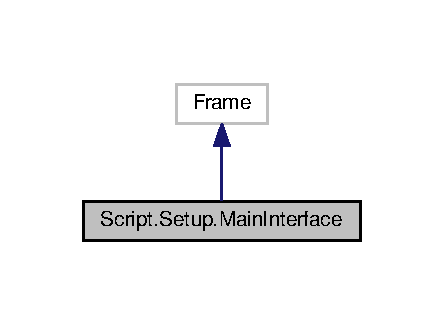
\includegraphics[width=213pt]{classScript_1_1Setup_1_1MainInterface__inherit__graph}
\end{center}
\end{figure}


Graphe de collaboration de Script.\+Setup.\+Main\+Interface\+:\nopagebreak
\begin{figure}[H]
\begin{center}
\leavevmode
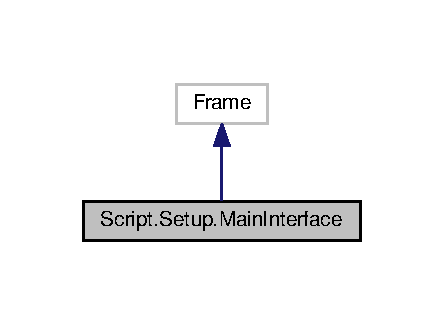
\includegraphics[width=213pt]{classScript_1_1Setup_1_1MainInterface__coll__graph}
\end{center}
\end{figure}
\subsection*{Fonctions membres publiques}
\begin{DoxyCompactItemize}
\item 
def \hyperlink{classScript_1_1Setup_1_1MainInterface_a342ef881ed8e49715e8e071026290d33}{\+\_\+\+\_\+init\+\_\+\+\_\+} (self, parent, kwargs)
\item 
def \hyperlink{classScript_1_1Setup_1_1MainInterface_aaa122e78c353c8b0014b07ff944d7818}{Init\+\_\+all\+\_\+frame} (self)
\item 
def \hyperlink{classScript_1_1Setup_1_1MainInterface_a92190b04a1cf9aa5497439f2dd6dcd99}{poll} (self)
\end{DoxyCompactItemize}
\subsection*{Attributs publics}
\begin{DoxyCompactItemize}
\item 
\hyperlink{classScript_1_1Setup_1_1MainInterface_a9436309be16e61a1527bdb8a62514de4}{root}
\item 
\hyperlink{classScript_1_1Setup_1_1MainInterface_a55c2c685b44f6ece1c4a9ea1eb8db30c}{select}
\item 
\hyperlink{classScript_1_1Setup_1_1MainInterface_a8ad532a968e6ccc0a5a1141d89b0bc79}{Frame1}
\item 
\hyperlink{classScript_1_1Setup_1_1MainInterface_a5e740f301b7cb8dd3fb145b6d0dc4af2}{Frame2}
\item 
\hyperlink{classScript_1_1Setup_1_1MainInterface_ab2dbe8bd2ef4977361a1a77c67648d3f}{Frame3}
\item 
\hyperlink{classScript_1_1Setup_1_1MainInterface_adbe875b37eb9ba01b2c84867dea6e526}{Frame4}
\end{DoxyCompactItemize}


\subsection{Description détaillée}


Définition à la ligne 18 du fichier Setup.\+py.



\subsection{Documentation des constructeurs et destructeur}
\mbox{\Hypertarget{classScript_1_1Setup_1_1MainInterface_a342ef881ed8e49715e8e071026290d33}\label{classScript_1_1Setup_1_1MainInterface_a342ef881ed8e49715e8e071026290d33}} 
\index{Script\+::\+Setup\+::\+Main\+Interface@{Script\+::\+Setup\+::\+Main\+Interface}!\+\_\+\+\_\+init\+\_\+\+\_\+@{\+\_\+\+\_\+init\+\_\+\+\_\+}}
\index{\+\_\+\+\_\+init\+\_\+\+\_\+@{\+\_\+\+\_\+init\+\_\+\+\_\+}!Script\+::\+Setup\+::\+Main\+Interface@{Script\+::\+Setup\+::\+Main\+Interface}}
\subsubsection{\texorpdfstring{\+\_\+\+\_\+init\+\_\+\+\_\+()}{\_\_init\_\_()}}
{\footnotesize\ttfamily def Script.\+Setup.\+Main\+Interface.\+\_\+\+\_\+init\+\_\+\+\_\+ (\begin{DoxyParamCaption}\item[{}]{self,  }\item[{}]{parent,  }\item[{}]{kwargs }\end{DoxyParamCaption})}



Définition à la ligne 19 du fichier Setup.\+py.


\begin{DoxyCode}
19     \textcolor{keyword}{def }\_\_init\_\_(self, parent, **kwargs):
20 
21         self.root = parent
22         self.root.title(\textcolor{stringliteral}{"Main frame"})
23         self.root.geometry=(\textcolor{stringliteral}{"320x240"})
24         Frame.\_\_init\_\_(self, parent, width=320, height=240, **kwargs)
25         self.pack(fill=BOTH)
26 
27         self.select= IntVar()
28         self.Init\_all\_frame()
29         \textcolor{comment}{#self.poll()
}
30         thread = threading.Thread(target=self.poll)
31         thread.daemon= \textcolor{keyword}{True}
32         thread.start()
33     
\end{DoxyCode}


\subsection{Documentation des fonctions membres}
\mbox{\Hypertarget{classScript_1_1Setup_1_1MainInterface_aaa122e78c353c8b0014b07ff944d7818}\label{classScript_1_1Setup_1_1MainInterface_aaa122e78c353c8b0014b07ff944d7818}} 
\index{Script\+::\+Setup\+::\+Main\+Interface@{Script\+::\+Setup\+::\+Main\+Interface}!Init\+\_\+all\+\_\+frame@{Init\+\_\+all\+\_\+frame}}
\index{Init\+\_\+all\+\_\+frame@{Init\+\_\+all\+\_\+frame}!Script\+::\+Setup\+::\+Main\+Interface@{Script\+::\+Setup\+::\+Main\+Interface}}
\subsubsection{\texorpdfstring{Init\+\_\+all\+\_\+frame()}{Init\_all\_frame()}}
{\footnotesize\ttfamily def Script.\+Setup.\+Main\+Interface.\+Init\+\_\+all\+\_\+frame (\begin{DoxyParamCaption}\item[{}]{self }\end{DoxyParamCaption})}



Définition à la ligne 34 du fichier Setup.\+py.


\begin{DoxyCode}
34     \textcolor{keyword}{def }Init\_all\_frame(self):
35         self.Frame1= Frame(self, width = self.winfo\_width())
36         self.Frame1.grid(column=0,row=0)
37         \textcolor{comment}{#self.Frame1.pack(side=TOP, padx=5, pady=5)
}
38 
39         self.Frame2= Frame(self, width = self.winfo\_width())
40         \textcolor{comment}{#self.Frame2.pack(side=TOP, padx=5, pady=5)
}
41         self.Frame2.grid(column=0,row=1)
42         
43         self.Frame3= Frame(self, width = self.winfo\_width())
44         \textcolor{comment}{#self.Frame3.pack(side=TOP, padx=5, pady=5)
}
45         self.Frame3.grid(column=0,row=2)
46         
47         self.Frame4= Frame(self, width = self.winfo\_width())
48         \textcolor{comment}{#self.Frame4.pack(side=TOP, padx=5, pady=5)
}
49         self.Frame4.grid(column=0,row=3)
50         \textcolor{comment}{#self.Frame5= Frame(self)
}
51         \textcolor{comment}{#self.Frame5.pack(side=TOP, padx=5, pady=5)
}
52 
53         interfaceFrame.Frame\_init\_option(self.Frame1, self.Frame2, self.Frame3)
54         interfaceFrame.Frame\_select\_com(self.Frame2, \textcolor{stringliteral}{"PTP"})
55         \textcolor{comment}{#interfaceFrame.Frame\_select\_file(self.Frame3, 1)
}
56         interfaceFrame.Frame\_btn\_execution(self.Frame4)
57 
58         \textcolor{comment}{#interfaceFrame.Frame\_resultat(self.Frame5)
}
59 
\end{DoxyCode}
\mbox{\Hypertarget{classScript_1_1Setup_1_1MainInterface_a92190b04a1cf9aa5497439f2dd6dcd99}\label{classScript_1_1Setup_1_1MainInterface_a92190b04a1cf9aa5497439f2dd6dcd99}} 
\index{Script\+::\+Setup\+::\+Main\+Interface@{Script\+::\+Setup\+::\+Main\+Interface}!poll@{poll}}
\index{poll@{poll}!Script\+::\+Setup\+::\+Main\+Interface@{Script\+::\+Setup\+::\+Main\+Interface}}
\subsubsection{\texorpdfstring{poll()}{poll()}}
{\footnotesize\ttfamily def Script.\+Setup.\+Main\+Interface.\+poll (\begin{DoxyParamCaption}\item[{}]{self }\end{DoxyParamCaption})}



Définition à la ligne 60 du fichier Setup.\+py.



Références Script.\+Setup.\+Main\+Interface.\+poll(), et Script.\+Setup.\+Main\+Interface.\+root.



Référencé par Script.\+Setup.\+Main\+Interface.\+poll().


\begin{DoxyCode}
60     \textcolor{keyword}{def }poll(self):
61         self.root.after(100,self.poll)
62 
63 
\end{DoxyCode}
Voici le graphe d\textquotesingle{}appel pour cette fonction \+:\nopagebreak
\begin{figure}[H]
\begin{center}
\leavevmode
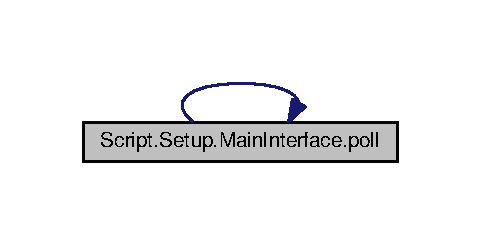
\includegraphics[width=231pt]{classScript_1_1Setup_1_1MainInterface_a92190b04a1cf9aa5497439f2dd6dcd99_cgraph}
\end{center}
\end{figure}
Voici le graphe des appelants de cette fonction \+:\nopagebreak
\begin{figure}[H]
\begin{center}
\leavevmode
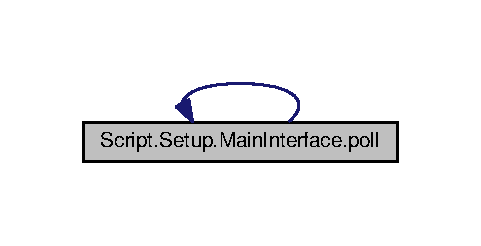
\includegraphics[width=231pt]{classScript_1_1Setup_1_1MainInterface_a92190b04a1cf9aa5497439f2dd6dcd99_icgraph}
\end{center}
\end{figure}


\subsection{Documentation des données membres}
\mbox{\Hypertarget{classScript_1_1Setup_1_1MainInterface_a8ad532a968e6ccc0a5a1141d89b0bc79}\label{classScript_1_1Setup_1_1MainInterface_a8ad532a968e6ccc0a5a1141d89b0bc79}} 
\index{Script\+::\+Setup\+::\+Main\+Interface@{Script\+::\+Setup\+::\+Main\+Interface}!Frame1@{Frame1}}
\index{Frame1@{Frame1}!Script\+::\+Setup\+::\+Main\+Interface@{Script\+::\+Setup\+::\+Main\+Interface}}
\subsubsection{\texorpdfstring{Frame1}{Frame1}}
{\footnotesize\ttfamily Script.\+Setup.\+Main\+Interface.\+Frame1}



Définition à la ligne 35 du fichier Setup.\+py.

\mbox{\Hypertarget{classScript_1_1Setup_1_1MainInterface_a5e740f301b7cb8dd3fb145b6d0dc4af2}\label{classScript_1_1Setup_1_1MainInterface_a5e740f301b7cb8dd3fb145b6d0dc4af2}} 
\index{Script\+::\+Setup\+::\+Main\+Interface@{Script\+::\+Setup\+::\+Main\+Interface}!Frame2@{Frame2}}
\index{Frame2@{Frame2}!Script\+::\+Setup\+::\+Main\+Interface@{Script\+::\+Setup\+::\+Main\+Interface}}
\subsubsection{\texorpdfstring{Frame2}{Frame2}}
{\footnotesize\ttfamily Script.\+Setup.\+Main\+Interface.\+Frame2}



Définition à la ligne 39 du fichier Setup.\+py.

\mbox{\Hypertarget{classScript_1_1Setup_1_1MainInterface_ab2dbe8bd2ef4977361a1a77c67648d3f}\label{classScript_1_1Setup_1_1MainInterface_ab2dbe8bd2ef4977361a1a77c67648d3f}} 
\index{Script\+::\+Setup\+::\+Main\+Interface@{Script\+::\+Setup\+::\+Main\+Interface}!Frame3@{Frame3}}
\index{Frame3@{Frame3}!Script\+::\+Setup\+::\+Main\+Interface@{Script\+::\+Setup\+::\+Main\+Interface}}
\subsubsection{\texorpdfstring{Frame3}{Frame3}}
{\footnotesize\ttfamily Script.\+Setup.\+Main\+Interface.\+Frame3}



Définition à la ligne 43 du fichier Setup.\+py.

\mbox{\Hypertarget{classScript_1_1Setup_1_1MainInterface_adbe875b37eb9ba01b2c84867dea6e526}\label{classScript_1_1Setup_1_1MainInterface_adbe875b37eb9ba01b2c84867dea6e526}} 
\index{Script\+::\+Setup\+::\+Main\+Interface@{Script\+::\+Setup\+::\+Main\+Interface}!Frame4@{Frame4}}
\index{Frame4@{Frame4}!Script\+::\+Setup\+::\+Main\+Interface@{Script\+::\+Setup\+::\+Main\+Interface}}
\subsubsection{\texorpdfstring{Frame4}{Frame4}}
{\footnotesize\ttfamily Script.\+Setup.\+Main\+Interface.\+Frame4}



Définition à la ligne 47 du fichier Setup.\+py.

\mbox{\Hypertarget{classScript_1_1Setup_1_1MainInterface_a9436309be16e61a1527bdb8a62514de4}\label{classScript_1_1Setup_1_1MainInterface_a9436309be16e61a1527bdb8a62514de4}} 
\index{Script\+::\+Setup\+::\+Main\+Interface@{Script\+::\+Setup\+::\+Main\+Interface}!root@{root}}
\index{root@{root}!Script\+::\+Setup\+::\+Main\+Interface@{Script\+::\+Setup\+::\+Main\+Interface}}
\subsubsection{\texorpdfstring{root}{root}}
{\footnotesize\ttfamily Script.\+Setup.\+Main\+Interface.\+root}



Définition à la ligne 21 du fichier Setup.\+py.



Référencé par Script.\+Setup.\+Main\+Interface.\+poll().

\mbox{\Hypertarget{classScript_1_1Setup_1_1MainInterface_a55c2c685b44f6ece1c4a9ea1eb8db30c}\label{classScript_1_1Setup_1_1MainInterface_a55c2c685b44f6ece1c4a9ea1eb8db30c}} 
\index{Script\+::\+Setup\+::\+Main\+Interface@{Script\+::\+Setup\+::\+Main\+Interface}!select@{select}}
\index{select@{select}!Script\+::\+Setup\+::\+Main\+Interface@{Script\+::\+Setup\+::\+Main\+Interface}}
\subsubsection{\texorpdfstring{select}{select}}
{\footnotesize\ttfamily Script.\+Setup.\+Main\+Interface.\+select}



Définition à la ligne 27 du fichier Setup.\+py.



La documentation de cette classe a été générée à partir du fichier suivant \+:\begin{DoxyCompactItemize}
\item 
\hyperlink{Setup_8py}{Setup.\+py}\end{DoxyCompactItemize}

\hypertarget{classScript_1_1handOver_1_1MobileReceives}{}\section{Référence de la classe Script.\+hand\+Over.\+Mobile\+Receives}
\label{classScript_1_1handOver_1_1MobileReceives}\index{Script.\+hand\+Over.\+Mobile\+Receives@{Script.\+hand\+Over.\+Mobile\+Receives}}


Graphe d\textquotesingle{}héritage de Script.\+hand\+Over.\+Mobile\+Receives\+:\nopagebreak
\begin{figure}[H]
\begin{center}
\leavevmode
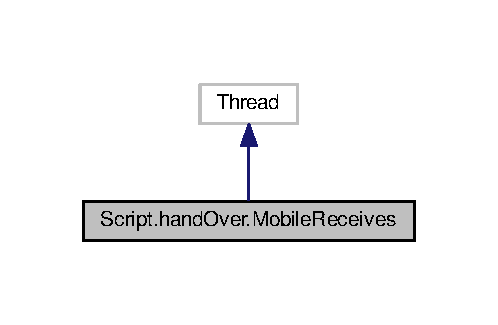
\includegraphics[width=239pt]{classScript_1_1handOver_1_1MobileReceives__inherit__graph}
\end{center}
\end{figure}


Graphe de collaboration de Script.\+hand\+Over.\+Mobile\+Receives\+:\nopagebreak
\begin{figure}[H]
\begin{center}
\leavevmode
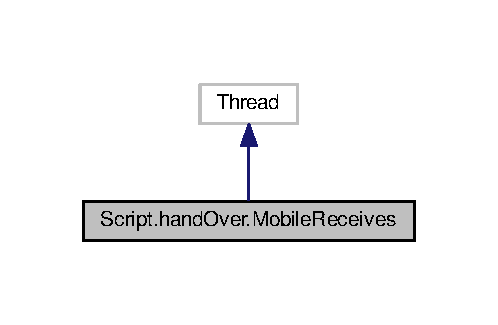
\includegraphics[width=239pt]{classScript_1_1handOver_1_1MobileReceives__coll__graph}
\end{center}
\end{figure}
\subsection*{Fonctions membres publiques}
\begin{DoxyCompactItemize}
\item 
def \hyperlink{classScript_1_1handOver_1_1MobileReceives_abb762c0c475770a14588d7005e1320da}{\+\_\+\+\_\+init\+\_\+\+\_\+} (self)
\item 
def \hyperlink{classScript_1_1handOver_1_1MobileReceives_a340893dfd7b7d84b3282bd0c24044e37}{run} (self)
\end{DoxyCompactItemize}
\subsection*{Attributs publics}
\begin{DoxyCompactItemize}
\item 
\hyperlink{classScript_1_1handOver_1_1MobileReceives_abb579ed112e4ce4e91762febd524d789}{phone}
\end{DoxyCompactItemize}


\subsection{Description détaillée}


Définition à la ligne 45 du fichier hand\+Over.\+py.



\subsection{Documentation des constructeurs et destructeur}
\mbox{\Hypertarget{classScript_1_1handOver_1_1MobileReceives_abb762c0c475770a14588d7005e1320da}\label{classScript_1_1handOver_1_1MobileReceives_abb762c0c475770a14588d7005e1320da}} 
\index{Script\+::hand\+Over\+::\+Mobile\+Receives@{Script\+::hand\+Over\+::\+Mobile\+Receives}!\+\_\+\+\_\+init\+\_\+\+\_\+@{\+\_\+\+\_\+init\+\_\+\+\_\+}}
\index{\+\_\+\+\_\+init\+\_\+\+\_\+@{\+\_\+\+\_\+init\+\_\+\+\_\+}!Script\+::hand\+Over\+::\+Mobile\+Receives@{Script\+::hand\+Over\+::\+Mobile\+Receives}}
\subsubsection{\texorpdfstring{\+\_\+\+\_\+init\+\_\+\+\_\+()}{\_\_init\_\_()}}
{\footnotesize\ttfamily def Script.\+hand\+Over.\+Mobile\+Receives.\+\_\+\+\_\+init\+\_\+\+\_\+ (\begin{DoxyParamCaption}\item[{}]{self }\end{DoxyParamCaption})}



Définition à la ligne 47 du fichier hand\+Over.\+py.


\begin{DoxyCode}
47     \textcolor{keyword}{def }\_\_init\_\_(self):
48         Thread.\_\_init\_\_(self)
49         with VERROU:
50             self.phone= serial.Serial(interfaceFrame.VALUE\_BOX\_COM2.get(), baudrate, timeout=1)
51         \textcolor{keywordflow}{if} self.phone.isOpen():
52             \textcolor{comment}{# On envoi cette command pour dire au mobile de decrocher automatique les appels data
}
53             self.phone.write(b\textcolor{stringliteral}{"ATS0=1\(\backslash\)r"})
\end{DoxyCode}


\subsection{Documentation des fonctions membres}
\mbox{\Hypertarget{classScript_1_1handOver_1_1MobileReceives_a340893dfd7b7d84b3282bd0c24044e37}\label{classScript_1_1handOver_1_1MobileReceives_a340893dfd7b7d84b3282bd0c24044e37}} 
\index{Script\+::hand\+Over\+::\+Mobile\+Receives@{Script\+::hand\+Over\+::\+Mobile\+Receives}!run@{run}}
\index{run@{run}!Script\+::hand\+Over\+::\+Mobile\+Receives@{Script\+::hand\+Over\+::\+Mobile\+Receives}}
\subsubsection{\texorpdfstring{run()}{run()}}
{\footnotesize\ttfamily def Script.\+hand\+Over.\+Mobile\+Receives.\+run (\begin{DoxyParamCaption}\item[{}]{self }\end{DoxyParamCaption})}



Définition à la ligne 54 du fichier hand\+Over.\+py.



Références Script.\+hand\+Over.\+Mobile\+Receives.\+phone.


\begin{DoxyCode}
54     \textcolor{keyword}{def }run(self):
55         \textcolor{keyword}{global} RELEASE
56         \textcolor{keyword}{global} RING\_STATUS
57         RELEASE= \textcolor{keyword}{False}
58         time.sleep(2)
59         \textcolor{comment}{# On verifie le port COM est bien etablit pour eviter des bug
}
60         \textcolor{keywordflow}{if} self.phone.isOpen():
61             with VERROU:
62                 \textcolor{comment}{# On initialise le mobile à une vitesse que l'utilisateur à déja definie
}
63                 self.phone.write(b\textcolor{stringliteral}{"AT+CBST="}+interfaceFrame.VALUE\_ENTRY\_ATCBST.get()+b\textcolor{stringliteral}{'\(\backslash\)r'})
64             time.sleep(3)
65             with VERROU:
66                 self.phone.readlines()
67             \textcolor{comment}{# On verifie que l'utilisateur n'a pas fermer la barre de progression
}
68             \textcolor{keywordflow}{while} Option.RUNNING == \textcolor{keyword}{True}:
69                 \textcolor{comment}{# On met cette variable à true pour que le mobile recoit un appel
}
70                 \textcolor{keywordflow}{if} RING\_STATUS == \textcolor{keyword}{True}:
71                     time.sleep(3)
72                     \textcolor{comment}{# On recuperer la reponse retouner par le telephone
}
73                     reponse= Option.split\_chaine(self.phone.readlines(), \textcolor{stringliteral}{""})
74                     \textcolor{comment}{# On verifie qu'on a bien connect entre les mobiles
}
75                     \textcolor{keywordflow}{if} (reponse.find(\textcolor{stringliteral}{"CONNECT"}) != -1) \textcolor{keywordflow}{or} (reponse.find(\textcolor{stringliteral}{"CONNECT"}) != -1):
76                         RING\_STATUS= \textcolor{keyword}{False}
77                     \textcolor{keywordflow}{else}:
78                         with VERROU:
79                             \textcolor{comment}{# On envoie cette commande pour que le mobile decrocher l'appel voix
}
80                             self.phone.write(b\textcolor{stringliteral}{"ATA\(\backslash\)r"})
81                             time.sleep(2)
82                         RING\_STATUS= \textcolor{keyword}{False}
83                 \textcolor{keywordflow}{if} RELEASE == \textcolor{keyword}{True}:
84                     \textcolor{comment}{# on envoie la commande pour que le mobile arrête le groupe call
}
85                     self.phone.write(b\textcolor{stringliteral}{'at+vts="*","*","*"\(\backslash\)r'})
86                     RELEASE= \textcolor{keyword}{False}
87             with VERROU:
88                 self.phone.close()
89         \textcolor{keywordflow}{else}:
90             print(\textcolor{stringliteral}{"Can not open '"}+interfaceFrame.VALUE\_BOX\_COM2.get())
91 
92 
93 \textcolor{comment}{# Cette correspond au mobile qui émet l'appel
}
94 \textcolor{comment}{# Est une thread pour pralleliser les information 
}
95 \textcolor{comment}{# elle s'ocuper e l'exécution des appels ptp, data, rec, vsb, data
}
96 \textcolor{comment}{# elle verifie le type d'appel choisi par l'utilisateur
}
97 
\end{DoxyCode}


\subsection{Documentation des données membres}
\mbox{\Hypertarget{classScript_1_1handOver_1_1MobileReceives_abb579ed112e4ce4e91762febd524d789}\label{classScript_1_1handOver_1_1MobileReceives_abb579ed112e4ce4e91762febd524d789}} 
\index{Script\+::hand\+Over\+::\+Mobile\+Receives@{Script\+::hand\+Over\+::\+Mobile\+Receives}!phone@{phone}}
\index{phone@{phone}!Script\+::hand\+Over\+::\+Mobile\+Receives@{Script\+::hand\+Over\+::\+Mobile\+Receives}}
\subsubsection{\texorpdfstring{phone}{phone}}
{\footnotesize\ttfamily Script.\+hand\+Over.\+Mobile\+Receives.\+phone}



Définition à la ligne 50 du fichier hand\+Over.\+py.



Référencé par Script.\+hand\+Over.\+Mobile\+Transmitter.\+data(), Script.\+hand\+Over.\+Mobile\+Transmitter.\+group\+\_\+call(), Script.\+hand\+Over.\+Mobile\+Transmitter.\+ptp(), et Script.\+hand\+Over.\+Mobile\+Receives.\+run().



La documentation de cette classe a été générée à partir du fichier suivant \+:\begin{DoxyCompactItemize}
\item 
\hyperlink{handOver_8py}{hand\+Over.\+py}\end{DoxyCompactItemize}

\hypertarget{classScript_1_1handOver_1_1MobileTransmitter}{}\section{Référence de la classe Script.\+hand\+Over.\+Mobile\+Transmitter}
\label{classScript_1_1handOver_1_1MobileTransmitter}\index{Script.\+hand\+Over.\+Mobile\+Transmitter@{Script.\+hand\+Over.\+Mobile\+Transmitter}}


Graphe d\textquotesingle{}héritage de Script.\+hand\+Over.\+Mobile\+Transmitter\+:\nopagebreak
\begin{figure}[H]
\begin{center}
\leavevmode
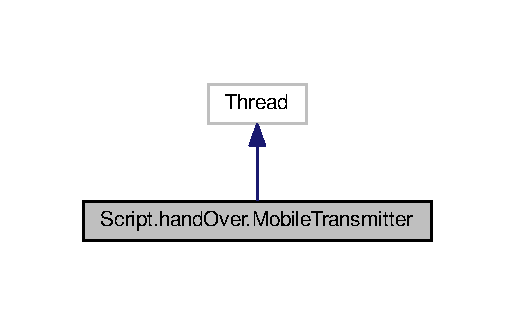
\includegraphics[width=247pt]{classScript_1_1handOver_1_1MobileTransmitter__inherit__graph}
\end{center}
\end{figure}


Graphe de collaboration de Script.\+hand\+Over.\+Mobile\+Transmitter\+:\nopagebreak
\begin{figure}[H]
\begin{center}
\leavevmode
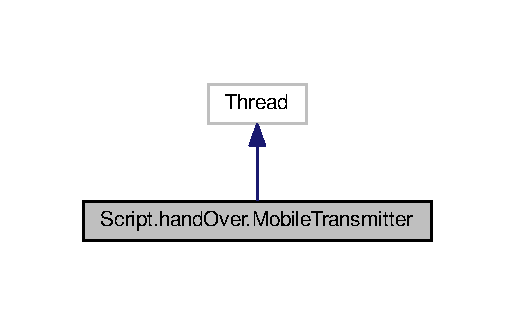
\includegraphics[width=247pt]{classScript_1_1handOver_1_1MobileTransmitter__coll__graph}
\end{center}
\end{figure}
\subsection*{Fonctions membres publiques}
\begin{DoxyCompactItemize}
\item 
def \hyperlink{classScript_1_1handOver_1_1MobileTransmitter_a2d85711a89b1b99cadb9d759d1d6072f}{\+\_\+\+\_\+init\+\_\+\+\_\+} (self, simple, tmu, \hyperlink{classScript_1_1handOver_1_1MobileTransmitter_a0cb158c80c1244e3379fe4eb91dad8fd}{ptp}, \hyperlink{classScript_1_1handOver_1_1MobileTransmitter_a5a0e39e384fabd4381f93ec60be74616}{data}, vgcs, rec, vbs)
\item 
def \hyperlink{classScript_1_1handOver_1_1MobileTransmitter_a0cb158c80c1244e3379fe4eb91dad8fd}{ptp} (self, tmu\+\_\+mode)
\item 
def \hyperlink{classScript_1_1handOver_1_1MobileTransmitter_a5a0e39e384fabd4381f93ec60be74616}{data} (self, tmu\+\_\+mode)
\item 
def \hyperlink{classScript_1_1handOver_1_1MobileTransmitter_aa94147ba15169a9f22363e2bab2e5cd9}{group\+\_\+call} (self, type\+\_\+call, tmu\+\_\+mode)
\item 
def \hyperlink{classScript_1_1handOver_1_1MobileTransmitter_aec021d2c9b7b289d100a056e21a730b8}{run} (self)
\end{DoxyCompactItemize}
\subsection*{Attributs publics}
\begin{DoxyCompactItemize}
\item 
\hyperlink{classScript_1_1handOver_1_1MobileTransmitter_a1f16581fb004249e79e9e62f081cb587}{S\+I\+M\+P\+LE}
\item 
\hyperlink{classScript_1_1handOver_1_1MobileTransmitter_a0a95c17a136be45d49aa83638edf2f0d}{R\+T\+MU}
\item 
\hyperlink{classScript_1_1handOver_1_1MobileTransmitter_a7fd1ea34ee9d8b66a96bb04fb56f1ed5}{P\+TP}
\item 
\hyperlink{classScript_1_1handOver_1_1MobileTransmitter_a078bbe0f45ce46f41e06f0faeb37cc1a}{D\+A\+TA}
\item 
\hyperlink{classScript_1_1handOver_1_1MobileTransmitter_accf8be809b557d3dda8ccdc9692f155e}{V\+G\+CS}
\item 
\hyperlink{classScript_1_1handOver_1_1MobileTransmitter_a16368e4843a51b1d473cf75c9ee71ff8}{R\+EC}
\item 
\hyperlink{classScript_1_1handOver_1_1MobileTransmitter_a38f03c3ffddd0e6b91ae0db987d4e79f}{V\+BS}
\item 
\hyperlink{classScript_1_1handOver_1_1MobileTransmitter_a5e7d14e9cab67b5af15e96b6451c8b35}{Filename}
\item 
\hyperlink{classScript_1_1handOver_1_1MobileTransmitter_a866608c9e27a57c84cea03fc1de1696f}{phone}
\item 
\hyperlink{classScript_1_1handOver_1_1MobileTransmitter_a364ca0783d420d2b1913646377ba0123}{H\+O\+\_\+\+O\+MC}
\item 
\hyperlink{classScript_1_1handOver_1_1MobileTransmitter_ae5933fac2e95221c47244fafcf33ff88}{H\+O\+\_\+\+O\+M\+U1}
\item 
\hyperlink{classScript_1_1handOver_1_1MobileTransmitter_aab1fb4256449d1379f82f6e7e741f8c0}{H\+O\+\_\+\+O\+M\+U2}
\item 
\hyperlink{classScript_1_1handOver_1_1MobileTransmitter_a3af626813f1fb97a4dfbd264f032fcc8}{N\+B\+R\+T\+MU}
\end{DoxyCompactItemize}


\subsection{Description détaillée}


Définition à la ligne 98 du fichier hand\+Over.\+py.



\subsection{Documentation des constructeurs et destructeur}
\mbox{\Hypertarget{classScript_1_1handOver_1_1MobileTransmitter_a2d85711a89b1b99cadb9d759d1d6072f}\label{classScript_1_1handOver_1_1MobileTransmitter_a2d85711a89b1b99cadb9d759d1d6072f}} 
\index{Script\+::hand\+Over\+::\+Mobile\+Transmitter@{Script\+::hand\+Over\+::\+Mobile\+Transmitter}!\+\_\+\+\_\+init\+\_\+\+\_\+@{\+\_\+\+\_\+init\+\_\+\+\_\+}}
\index{\+\_\+\+\_\+init\+\_\+\+\_\+@{\+\_\+\+\_\+init\+\_\+\+\_\+}!Script\+::hand\+Over\+::\+Mobile\+Transmitter@{Script\+::hand\+Over\+::\+Mobile\+Transmitter}}
\subsubsection{\texorpdfstring{\+\_\+\+\_\+init\+\_\+\+\_\+()}{\_\_init\_\_()}}
{\footnotesize\ttfamily def Script.\+hand\+Over.\+Mobile\+Transmitter.\+\_\+\+\_\+init\+\_\+\+\_\+ (\begin{DoxyParamCaption}\item[{}]{self,  }\item[{}]{simple,  }\item[{}]{tmu,  }\item[{}]{ptp,  }\item[{}]{data,  }\item[{}]{vgcs,  }\item[{}]{rec,  }\item[{}]{vbs }\end{DoxyParamCaption})}



Définition à la ligne 100 du fichier hand\+Over.\+py.


\begin{DoxyCode}
100     \textcolor{keyword}{def }\_\_init\_\_(self, simple, tmu, ptp, data, vgcs, rec, vbs):
101         Thread.\_\_init\_\_(self)
102         self.SIMPLE= simple
103         self.RTMU= tmu
104         self.PTP= ptp
105         self.DATA= data
106         self.VGCS= vgcs
107         self.REC= rec
108         self.VBS= vbs
109         self.Filename= open(os.path.dirname(\_\_file\_\_)+\textcolor{stringliteral}{"/../File/Rapport.txt"}, \textcolor{stringliteral}{"w"})
110         
111         with VERROU:
112             self.phone= serial.Serial(interfaceFrame.VALUE\_BOX\_COM1.get(), baudrate, timeout=1)
113 
\end{DoxyCode}


\subsection{Documentation des fonctions membres}
\mbox{\Hypertarget{classScript_1_1handOver_1_1MobileTransmitter_a5a0e39e384fabd4381f93ec60be74616}\label{classScript_1_1handOver_1_1MobileTransmitter_a5a0e39e384fabd4381f93ec60be74616}} 
\index{Script\+::hand\+Over\+::\+Mobile\+Transmitter@{Script\+::hand\+Over\+::\+Mobile\+Transmitter}!data@{data}}
\index{data@{data}!Script\+::hand\+Over\+::\+Mobile\+Transmitter@{Script\+::hand\+Over\+::\+Mobile\+Transmitter}}
\subsubsection{\texorpdfstring{data()}{data()}}
{\footnotesize\ttfamily def Script.\+hand\+Over.\+Mobile\+Transmitter.\+data (\begin{DoxyParamCaption}\item[{}]{self,  }\item[{}]{tmu\+\_\+mode }\end{DoxyParamCaption})}



Définition à la ligne 192 du fichier hand\+Over.\+py.



Références Script.\+hand\+Over.\+Mobile\+Transmitter.\+Filename, Script.\+hand\+Over.\+Mobile\+Transmitter.\+H\+O\+\_\+\+O\+MC, Script.\+hand\+Over.\+Mobile\+Transmitter.\+H\+O\+\_\+\+O\+M\+U1, Script.\+hand\+Over.\+Mobile\+Transmitter.\+H\+O\+\_\+\+O\+M\+U2, Script.\+hand\+Over.\+Mobile\+Transmitter.\+N\+B\+R\+T\+MU, Script.\+hand\+Over.\+Mobile\+Receives.\+phone, et Script.\+hand\+Over.\+Mobile\+Transmitter.\+phone.


\begin{DoxyCode}
192     \textcolor{keyword}{def }data(self, tmu\_mode):
193         \textcolor{keyword}{global} RING\_STATUS
194         connect\_phone=\textcolor{keyword}{False}
195         nb\_atd= 5
196 
197 
198         \textcolor{keywordflow}{if} self.phone.isOpen():
199             self.phone.readlines()
200             with VERROU:
201                 self.phone.write(b\textcolor{stringliteral}{"ATD"}+interfaceFrame.VALUE\_ENTRY\_PHONE\_NUMERO.get()+b\textcolor{stringliteral}{'\(\backslash\)r'})
202                 time.sleep(2)
203             \textcolor{keywordflow}{while} nb\_atd > 0:
204                 time.sleep(10)
205                 with VERROU:
206                     reponse= Option.split\_chaine(self.phone.readlines(), \textcolor{stringliteral}{""})
207                     time.sleep(2)
208                 \textcolor{keywordflow}{if} (reponse.find(\textcolor{stringliteral}{"OK"}) != -1):
209                     RING\_STATUS = \textcolor{keyword}{True}
210                     \textcolor{keywordflow}{break}
211                 \textcolor{keywordflow}{if} (reponse.find(\textcolor{stringliteral}{"CONNECT"}) != -1):
212                     RING\_STATUS= \textcolor{keyword}{False}
213                     connect\_phone= \textcolor{keyword}{True}
214                     \textcolor{keywordflow}{break}
215                 \textcolor{keywordflow}{else}:
216                     with VERROU:
217                         self.phone.write(b\textcolor{stringliteral}{"ATD"}+interfaceFrame.VALUE\_ENTRY\_PHONE\_NUMERO.get()+b\textcolor{stringliteral}{'\(\backslash\)r'})
218                         time.sleep(2)
219                 nb\_atd-=1
220             
221             \textcolor{keywordflow}{if} nb\_atd > 0:
222                 time.sleep(30)
223                 
224                 \textcolor{keywordflow}{while} \textcolor{keyword}{True}: \textcolor{comment}{#il faut un tempo le temps d'attente max
}
225                     reponse= Option.split\_chaine(self.phone.readlines(), \textcolor{stringliteral}{""})
226                     \textcolor{keywordflow}{if} (reponse.find(\textcolor{stringliteral}{"CONNECT"}) != -1) \textcolor{keywordflow}{or} (connect\_phone == \textcolor{keyword}{True}):
227                         print(reponse)
228                         connect\_phone= \textcolor{keyword}{True}
229                         \textcolor{keywordflow}{break}
230                     \textcolor{keywordflow}{if} reponse.find(\textcolor{stringliteral}{"NETWORK OUT OF ORDER"}) != -1:
231                         print(reponse)
232                         connect\_phone= \textcolor{keyword}{False}
233                         \textcolor{keywordflow}{break}
234                     \textcolor{comment}{#mise a jour du delai d'attente
}
235 
236                 \textcolor{keywordflow}{if} (connect\_phone==\textcolor{keyword}{True}) \textcolor{keywordflow}{and} (Option.RUNNING == \textcolor{keyword}{True}) \textcolor{keywordflow}{and} (RING\_STATUS ==\textcolor{keyword}{False}):
237                     
238                     
239                     \textcolor{keywordflow}{if} tmu\_mode == \textcolor{keyword}{True}:
240                         nb=1
241                         \textcolor{keywordflow}{while} nb <= self.NBRTMU:
242                             list\_tmu1= self.HO\_OMU1.get\_list\_tmu()
243                             list\_tmu2= self.HO\_OMU2.get\_list\_tmu()
244 
245                             min\_size\_tmu= min(len(list\_tmu1), len(list\_tmu2))
246                             \textcolor{keywordflow}{for} i \textcolor{keywordflow}{in} range(min\_size\_tmu):
247                                 
248                                 state\_omu1= self.HO\_OMU1.reset\_tmu(list\_tmu1[i])
249                                 state\_omu2= self.HO\_OMU2.reset\_tmu(list\_tmu2[i])
250                                 time.sleep(120)
251                                 \textcolor{comment}{#with VERROU:
}
252                                 state\_ho = self.HO\_OMC.run\_senario(\textcolor{stringliteral}{"data"})
253                                 print(\textcolor{stringliteral}{"NB === "}, self.NBRTMU)
254                                 text\_save=str(nb)+\textcolor{stringliteral}{" - CALL: DATA; MODE: RTMU; OMU1: "}+state\_omu1+\textcolor{stringliteral}{"; OMU2: "}
      +state\_omu1+\textcolor{stringliteral}{"; HandOver: "}+state\_ho+\textcolor{stringliteral}{";\(\backslash\)n"}                                
255                                 print(text\_save)
256                                 self.Filename.write(text\_save)
257                             nb+=1
258                     \textcolor{keywordflow}{else}:
259 
260                         state\_ho = self.HO\_OMC.run\_senario(\textcolor{stringliteral}{"data"})
261                         text\_save=\textcolor{stringliteral}{"0 - CaLL: DATA; MODE: SiMPLE; HANDOVER: "}+state\_ho+\textcolor{stringliteral}{";\(\backslash\)n"}
262                         print(text\_save)
263                         self.Filename.write(text\_save)
264 
265                     connect\_phone= \textcolor{keyword}{False}
266                     Option.hang\_up\_call(self.phone)
267                 \textcolor{keywordflow}{else}:
268                     print(\textcolor{stringliteral}{"impossible d'etablir un connect"})
269 
270             \textcolor{keywordflow}{else}:
271                 print(\textcolor{stringliteral}{"atd"}+interfaceFrame.VALUE\_ENTRY\_PHONE\_NUMERO.get()+\textcolor{stringliteral}{" ERROR\(\backslash\)n"})
272         \textcolor{keywordflow}{else}:
273             print(\textcolor{stringliteral}{"Can not open '"}+interfaceFrame.VALUE\_BOX\_COM1.get())
274 
275 
276 
277 
\end{DoxyCode}
\mbox{\Hypertarget{classScript_1_1handOver_1_1MobileTransmitter_aa94147ba15169a9f22363e2bab2e5cd9}\label{classScript_1_1handOver_1_1MobileTransmitter_aa94147ba15169a9f22363e2bab2e5cd9}} 
\index{Script\+::hand\+Over\+::\+Mobile\+Transmitter@{Script\+::hand\+Over\+::\+Mobile\+Transmitter}!group\+\_\+call@{group\+\_\+call}}
\index{group\+\_\+call@{group\+\_\+call}!Script\+::hand\+Over\+::\+Mobile\+Transmitter@{Script\+::hand\+Over\+::\+Mobile\+Transmitter}}
\subsubsection{\texorpdfstring{group\+\_\+call()}{group\_call()}}
{\footnotesize\ttfamily def Script.\+hand\+Over.\+Mobile\+Transmitter.\+group\+\_\+call (\begin{DoxyParamCaption}\item[{}]{self,  }\item[{}]{type\+\_\+call,  }\item[{}]{tmu\+\_\+mode }\end{DoxyParamCaption})}



Définition à la ligne 278 du fichier hand\+Over.\+py.



Références Script.\+hand\+Over.\+Mobile\+Transmitter.\+Filename, Script.\+hand\+Over.\+Mobile\+Transmitter.\+H\+O\+\_\+\+O\+MC, Script.\+hand\+Over.\+Mobile\+Transmitter.\+H\+O\+\_\+\+O\+M\+U1, Script.\+hand\+Over.\+Mobile\+Transmitter.\+H\+O\+\_\+\+O\+M\+U2, Script.\+hand\+Over.\+Mobile\+Transmitter.\+N\+B\+R\+T\+MU, Script.\+hand\+Over.\+Mobile\+Receives.\+phone, et Script.\+hand\+Over.\+Mobile\+Transmitter.\+phone.


\begin{DoxyCode}
278     \textcolor{keyword}{def }group\_call(self, type\_call, tmu\_mode):
279         \textcolor{keyword}{global} RING\_STATUS
280         \textcolor{keyword}{global} RELEASE
281         RELEASE= \textcolor{keyword}{False}
282 
283         nb\_atd= 5
284         \textcolor{keywordflow}{if} self.phone.isOpen():
285             str\_cmd\_call=\textcolor{stringliteral}{""}
286             \textcolor{keywordflow}{if} type\_call == \textcolor{stringliteral}{"vgcs"}:
287                 str\_cmd\_call=\textcolor{stringliteral}{"ATD*17*75#"}+interfaceFrame.VALUE\_ENTRY\_GROUP\_ID.get()+\textcolor{stringliteral}{";\(\backslash\)r"}
288             \textcolor{keywordflow}{elif} type\_call == \textcolor{stringliteral}{"rec"}:
289                 str\_cmd\_call=\textcolor{stringliteral}{"ATD*17*750#299;\(\backslash\)r"}
290             \textcolor{keywordflow}{elif} type\_call == \textcolor{stringliteral}{"vbs"}:
291                 str\_cmd\_call = \textcolor{stringliteral}{"ATD*18*75#"}+interfaceFrame.VALUE\_ENTRY\_GROUP\_ID.get()+\textcolor{stringliteral}{";\(\backslash\)r"}
292             \textcolor{keywordflow}{else}:
293                 \textcolor{keywordflow}{return} \textcolor{keywordtype}{None}
294             self.phone.readlines()
295             with VERROU:
296                 self.phone.write(b\textcolor{stringliteral}{""}+str\_cmd\_call)
297                 time.sleep(2)
298                 
299 
300             \textcolor{keywordflow}{while} nb\_atd > -1:
301                 time.sleep(3)
302                 with VERROU:
303                     reponse= Option.split\_chaine(self.phone.readlines(), \textcolor{stringliteral}{""})
304 
305                 \textcolor{keywordflow}{if} reponse.find(\textcolor{stringliteral}{"OK"}) != -1:
306                     RING\_STATUS = \textcolor{keyword}{True}
307                     \textcolor{keywordflow}{break}
308                 \textcolor{keywordflow}{else}:
309                     with VERROU:
310                         self.phone.write(b\textcolor{stringliteral}{""}+str\_cmd\_call)
311                         time.sleep(2)
312 
313                 nb\_atd -=1
314             
315             \textcolor{keywordflow}{if} nb\_atd > -1:
316                 time.sleep(20)
317                 \textcolor{comment}{#if type\_call != "rec":
}
318                 \textcolor{comment}{#   suiv= raw\_input('Veuillez accepter le groupe call et appuyer sur entrer: ')
}
319                 reponse= Option.split\_chaine(self.phone.readlines(), \textcolor{stringliteral}{""})
320                 connect\_phone= \textcolor{keyword}{True}
321 
322                 \textcolor{keywordflow}{if} (RING\_STATUS== \textcolor{keyword}{False}) \textcolor{keywordflow}{and} (Option.RUNNING == \textcolor{keyword}{True}):
323                     nb=1
324                     \textcolor{keywordflow}{if} tmu\_mode == \textcolor{keyword}{True}:
325                         \textcolor{keywordflow}{while} nb <= self.NBRTMU:
326                             list\_tmu1= self.HO\_OMU1.get\_list\_tmu()
327                             list\_tmu2= self.HO\_OMU2.get\_list\_tmu()
328 
329                             min\_size\_tmu= min(len(list\_tmu1), len(list\_tmu2))
330                             \textcolor{keywordflow}{for} i \textcolor{keywordflow}{in} range(min\_size\_tmu):
331 
332                                 state\_omu1= self.HO\_OMU1.reset\_tmu(list\_tmu1[i])
333                                 state\_omu2= self.HO\_OMU2.reset\_tmu(list\_tmu2[i])
334                                 time.sleep(120)
335                                 \textcolor{comment}{#with VERROU:
}
336                                 state\_ho =self.HO\_OMC.run\_senario(type\_call)
337                                 
338                                 text\_save=str(nb)+\textcolor{stringliteral}{" - CALL: "}+type\_call+\textcolor{stringliteral}{"; MODE: RTMU; OMU1: "}+state\_omu1+\textcolor{stringliteral}{"
      ; OMU2: "}+state\_omu2+\textcolor{stringliteral}{"; HandOver: "}+state\_ho+\textcolor{stringliteral}{";\(\backslash\)n"}
339                                 print(text\_save)
340                                 self.Filename.write(text\_save)
341                             nb+=1
342                     \textcolor{keywordflow}{else}:
343                         state\_ho= self.HO\_OMC.run\_senario(type\_call)
344                         text\_save=\textcolor{stringliteral}{"0 - CALL: "}+type\_call+\textcolor{stringliteral}{"; MODE: SiMPLE; HANDOVER: "}+state\_ho+\textcolor{stringliteral}{";\(\backslash\)n"}
345                         print(text\_save)
346                         self.Filename.write(text\_save)
347                     RELEASE = \textcolor{keyword}{True}
348                     connect\_phone= \textcolor{keyword}{False}
349                     time.sleep(10)
350                     with VERROU:
351                         self.phone.write(b\textcolor{stringliteral}{"ATH\(\backslash\)r"})
352                     time.sleep(2)
353                     \textcolor{comment}{#suiv= raw\_input('Veuillez Kill le groupe call et appuyer sur entrer: ')
}
354                     RELEASE= \textcolor{keyword}{False}
355 
356             \textcolor{keywordflow}{else}:
357                 print(\textcolor{stringliteral}{"atd"}+interfaceFrame.VALUE\_ENTRY\_PHONE\_NUMERO.get()+\textcolor{stringliteral}{" ERROR\(\backslash\)n"})
358         \textcolor{keywordflow}{else}:
359             print(\textcolor{stringliteral}{"Can not open '"}+interfaceFrame.VALUE\_BOX\_COM1.get())
360 
361 
362 
363 
364 
\end{DoxyCode}
\mbox{\Hypertarget{classScript_1_1handOver_1_1MobileTransmitter_a0cb158c80c1244e3379fe4eb91dad8fd}\label{classScript_1_1handOver_1_1MobileTransmitter_a0cb158c80c1244e3379fe4eb91dad8fd}} 
\index{Script\+::hand\+Over\+::\+Mobile\+Transmitter@{Script\+::hand\+Over\+::\+Mobile\+Transmitter}!ptp@{ptp}}
\index{ptp@{ptp}!Script\+::hand\+Over\+::\+Mobile\+Transmitter@{Script\+::hand\+Over\+::\+Mobile\+Transmitter}}
\subsubsection{\texorpdfstring{ptp()}{ptp()}}
{\footnotesize\ttfamily def Script.\+hand\+Over.\+Mobile\+Transmitter.\+ptp (\begin{DoxyParamCaption}\item[{}]{self,  }\item[{}]{tmu\+\_\+mode }\end{DoxyParamCaption})}



Définition à la ligne 116 du fichier hand\+Over.\+py.



Références Script.\+hand\+Over.\+Mobile\+Transmitter.\+Filename, Script.\+hand\+Over.\+Mobile\+Transmitter.\+H\+O\+\_\+\+O\+MC, Script.\+hand\+Over.\+Mobile\+Transmitter.\+H\+O\+\_\+\+O\+M\+U1, Script.\+hand\+Over.\+Mobile\+Transmitter.\+H\+O\+\_\+\+O\+M\+U2, Script.\+hand\+Over.\+Mobile\+Transmitter.\+N\+B\+R\+T\+MU, Script.\+hand\+Over.\+Mobile\+Receives.\+phone, et Script.\+hand\+Over.\+Mobile\+Transmitter.\+phone.


\begin{DoxyCode}
116     \textcolor{keyword}{def }ptp(self, tmu\_mode):
117         \textcolor{keyword}{global} RING\_STATUS
118         nb\_atd= 5
119         connect\_phone=\textcolor{keyword}{False}
120 
121         \textcolor{keywordflow}{if} self.phone.isOpen():
122             self.phone.readlines()
123             with VERROU:
124                 \textcolor{comment}{# On compose le numéro du mobile qui réçoit l'appel
}
125                 self.phone.write(b\textcolor{stringliteral}{"ATD"}+interfaceFrame.VALUE\_ENTRY\_PHONE\_NUMERO.get()+b\textcolor{stringliteral}{";\(\backslash\)r"})
126                 time.sleep(2)
127 
128             \textcolor{keywordflow}{while} nb\_atd > -1:
129                 time.sleep(10)
130                 with VERROU:
131                     reponse= Option.split\_chaine(self.phone.readlines(), \textcolor{stringliteral}{""})
132 
133                     time.sleep(2)
134                 \textcolor{comment}{# On verifie que le numéro à bien été saisi 
}
135                 \textcolor{keywordflow}{if} reponse.find(\textcolor{stringliteral}{"OK"}) != -1:
136                     RING\_STATUS = \textcolor{keyword}{True}
137                     \textcolor{keywordflow}{break}
138                 \textcolor{keywordflow}{else}:
139                     with VERROU:
140                         \textcolor{comment}{# On verifie siasi à nouveau le nouveau du mobile qui réçoit l'appel
}
141                         self.phone.write(b\textcolor{stringliteral}{"ATD"}+interfaceFrame.VALUE\_ENTRY\_PHONE\_NUMERO.get()+b\textcolor{stringliteral}{";\(\backslash\)r"})
142                         time.sleep(2)
143                 nb\_atd -=1
144             
145             \textcolor{keywordflow}{if} nb\_atd > -1:
146                 time.sleep(30)
147                 reponse= Option.split\_chaine(self.phone.readlines(), \textcolor{stringliteral}{""})
148                 connect\_phone= \textcolor{keyword}{True}
149 
150                 \textcolor{keywordflow}{if} (RING\_STATUS== \textcolor{keyword}{False}) \textcolor{keywordflow}{and} (Option.RUNNING == \textcolor{keyword}{True}):
151                     nb=1
152                     \textcolor{keywordflow}{if} tmu\_mode == \textcolor{keyword}{True}:
153                         \textcolor{keywordflow}{while} nb <= self.NBRTMU:
154                             \textcolor{comment}{# On recupère la liste de tmu présent dans l'OMC pour les deux BSC
}
155                             list\_tmu1= self.HO\_OMU1.get\_list\_tmu()
156                             list\_tmu2= self.HO\_OMU2.get\_list\_tmu()
157 
158                             min\_size\_tmu= min(len(list\_tmu1), len(list\_tmu2))
159                             \textcolor{keywordflow}{for} i \textcolor{keywordflow}{in} range(min\_size\_tmu):
160                                 \textcolor{comment}{# On reset un tmu de chaque BSC et recupère les information rétourner sur
       l'exécution cette command
}
161                                 state\_omu1= self.HO\_OMU1.reset\_tmu(list\_tmu1[i])
162                                 state\_omu2= self.HO\_OMU2.reset\_tmu(list\_tmu2[i])
163                                 time.sleep(120)
164                                 \textcolor{comment}{#with VERROU:
}
165                                 \textcolor{comment}{# On éxécute le sénario avec
}
166                                 state\_ho =self.HO\_OMC.run\_senario(\textcolor{stringliteral}{"ptp"})
167                                 
168                                 text\_save=str(nb)+\textcolor{stringliteral}{" - CALL: PTP; MODE: RTMU; OMU1: "}+state\_omu1+\textcolor{stringliteral}{"; OMU2: "}+
      state\_omu2+\textcolor{stringliteral}{"; HandOver: "}+state\_ho+\textcolor{stringliteral}{";\(\backslash\)n"}
169                                 print(text\_save)
170                                 self.Filename.write(text\_save)
171                             nb+=1
172                     \textcolor{keywordflow}{else}:
173                         \textcolor{comment}{# On exécute le senarion de la voix sans faire le reset tmu
}
174                         state\_ho= self.HO\_OMC.run\_senario(\textcolor{stringliteral}{"ptp"})
175                         text\_save=\textcolor{stringliteral}{"0 - CaLL: PTP; MODE: SiMPLE; HANDOVER: "}+state\_ho+\textcolor{stringliteral}{";\(\backslash\)n"}
176                         print(text\_save)
177                         \textcolor{comment}{# On sauvegarde dans le fichier
}
178                         self.Filename.write(text\_save)
179 
180                     connect\_phone= \textcolor{keyword}{False}
181                     with VERROU:
182                         self.phone.write(b\textcolor{stringliteral}{"ATH\(\backslash\)r"})
183                         \textcolor{comment}{#print("ath")
}
184                     time.sleep(2)
185 
186             \textcolor{keywordflow}{else}:
187                 print(\textcolor{stringliteral}{"atd"}+interfaceFrame.VALUE\_ENTRY\_PHONE\_NUMERO.get()+\textcolor{stringliteral}{" ERROR\(\backslash\)n"})
188         \textcolor{keywordflow}{else}:
189             print(\textcolor{stringliteral}{"Can not open '"}+interfaceFrame.VALUE\_BOX\_COM1.get())
190 
191 
\end{DoxyCode}
\mbox{\Hypertarget{classScript_1_1handOver_1_1MobileTransmitter_aec021d2c9b7b289d100a056e21a730b8}\label{classScript_1_1handOver_1_1MobileTransmitter_aec021d2c9b7b289d100a056e21a730b8}} 
\index{Script\+::hand\+Over\+::\+Mobile\+Transmitter@{Script\+::hand\+Over\+::\+Mobile\+Transmitter}!run@{run}}
\index{run@{run}!Script\+::hand\+Over\+::\+Mobile\+Transmitter@{Script\+::hand\+Over\+::\+Mobile\+Transmitter}}
\subsubsection{\texorpdfstring{run()}{run()}}
{\footnotesize\ttfamily def Script.\+hand\+Over.\+Mobile\+Transmitter.\+run (\begin{DoxyParamCaption}\item[{}]{self }\end{DoxyParamCaption})}



Définition à la ligne 365 du fichier hand\+Over.\+py.


\begin{DoxyCode}
365     \textcolor{keyword}{def }run(self):
366         self.HO\_OMC = omc.OMC()
367 
368         with VERROU:
369             self.HO\_OMU1= omu.OMU(interfaceFrame.VALUE\_ENTRY\_OMU1\_IP.get(),\(\backslash\)
370                 interfaceFrame.VALUE\_ENTRY\_OMU1\_USER.get(),\(\backslash\)
371                 interfaceFrame.VALUE\_ENTRY\_OMU1\_PASSWORD.get())
372 
373         with VERROU:
374             self.HO\_OMU2= omu.OMU(interfaceFrame.VALUE\_ENTRY\_OMU2\_IP.get(),\(\backslash\)
375              interfaceFrame.VALUE\_ENTRY\_OMU2\_USER.get(),\(\backslash\)
376              interfaceFrame.VALUE\_ENTRY\_OMU2\_PASSWORD.get())
377 
378         \textcolor{keywordflow}{if} self.phone.isOpen():
379             with VERROU:
380                 self.phone.write(b\textcolor{stringliteral}{"AT+CBST="}+interfaceFrame.VALUE\_ENTRY\_ATCBST.get()+b\textcolor{stringliteral}{'\(\backslash\)r'})
381             time.sleep(3)
382             with VERROU:
383                 self.phone.readlines()
384 
385         \textcolor{keywordflow}{if} self.PTP == \textcolor{keyword}{True}:
386             \textcolor{keywordflow}{if} (self.SIMPLE == \textcolor{keyword}{True}) \textcolor{keywordflow}{and} (Option.RUNNING == \textcolor{keyword}{True}):
387                 print(\textcolor{stringliteral}{"ptp\_simple\_mode"})
388                 self.ptp(\textcolor{keyword}{False})
389 
390             \textcolor{keywordflow}{if} (self.RTMU == \textcolor{keyword}{True}) \textcolor{keywordflow}{and} (Option.RUNNING == \textcolor{keyword}{True}):
391                 self.NBRTMU = int(interfaceFrame.VALUE\_ENTRY\_NB\_RTMU.get())
392                 print(\textcolor{stringliteral}{"ptp\_tmu\_mode"})
393                 self.ptp(\textcolor{keyword}{True})
394 
395 
396         \textcolor{keywordflow}{if} self.DATA == \textcolor{keyword}{True}:
397             \textcolor{keywordflow}{if} (self.SIMPLE == \textcolor{keyword}{True}) \textcolor{keywordflow}{and} (Option.RUNNING == \textcolor{keyword}{True}):
398                 print(\textcolor{stringliteral}{"data\_simple\_mode"})
399                 self.data(\textcolor{keyword}{False})
400             \textcolor{keywordflow}{if} (self.RTMU == \textcolor{keyword}{True}) \textcolor{keywordflow}{and} (Option.RUNNING == \textcolor{keyword}{True}):
401                 self.NBRTMU = int(interfaceFrame.VALUE\_ENTRY\_NB\_RTMU.get())
402                 print(\textcolor{stringliteral}{"data\_tmu\_mode"})
403                 self.data(\textcolor{keyword}{True})
404 
405         \textcolor{keywordflow}{if} self.VGCS == \textcolor{keyword}{True}:
406             \textcolor{keywordflow}{if} (self.SIMPLE == \textcolor{keyword}{True}) \textcolor{keywordflow}{and} (Option.RUNNING == \textcolor{keyword}{True}):
407                 print(\textcolor{stringliteral}{"vgcs\_simple\_mode"})
408                 self.group\_call(\textcolor{stringliteral}{"vgcs"},\textcolor{keyword}{False})
409 
410             \textcolor{keywordflow}{if} (self.RTMU == \textcolor{keyword}{True}) \textcolor{keywordflow}{and} (Option.RUNNING == \textcolor{keyword}{True}):
411                 self.NBRTMU = int(interfaceFrame.VALUE\_ENTRY\_NB\_RTMU.get())
412                 print(\textcolor{stringliteral}{"vgcs\_tmu\_mode"})
413                 self.group\_call(\textcolor{stringliteral}{"vgcs"},\textcolor{keyword}{True})
414 
415 
416         \textcolor{keywordflow}{if} self.REC == \textcolor{keyword}{True}:
417             \textcolor{keywordflow}{if} (self.SIMPLE == \textcolor{keyword}{True}) \textcolor{keywordflow}{and} (Option.RUNNING == \textcolor{keyword}{True}):
418                 print(\textcolor{stringliteral}{"rec\_simple\_mode"})
419                 self.group\_call(\textcolor{stringliteral}{"rec"},\textcolor{keyword}{False})
420 
421             \textcolor{keywordflow}{if} (self.RTMU == \textcolor{keyword}{True}) \textcolor{keywordflow}{and} (Option.RUNNING == \textcolor{keyword}{True}):
422                 self.NBRTMU = int(interfaceFrame.VALUE\_ENTRY\_NB\_RTMU.get())
423                 print(\textcolor{stringliteral}{"rtmu\_tmu\_mode"})
424                 self.group\_call(\textcolor{stringliteral}{"rec"},\textcolor{keyword}{True})
425 
426 
427         \textcolor{keywordflow}{if} self.VBS == \textcolor{keyword}{True}:
428             \textcolor{keywordflow}{if} (self.SIMPLE == \textcolor{keyword}{True}) \textcolor{keywordflow}{and} (Option.RUNNING == \textcolor{keyword}{True}):
429                 print(\textcolor{stringliteral}{"vbs\_simple\_mode"})
430                 self.group\_call(\textcolor{stringliteral}{"vbs"},\textcolor{keyword}{False})
431 
432             \textcolor{keywordflow}{if} (self.RTMU == \textcolor{keyword}{True}) \textcolor{keywordflow}{and} (Option.RUNNING == \textcolor{keyword}{True}):
433                 self.NBRTMU = int(interfaceFrame.VALUE\_ENTRY\_NB\_RTMU.get())
434                 print(\textcolor{stringliteral}{"vbs\_tmu\_mode"})
435                 self.group\_call(\textcolor{stringliteral}{"vbs"},\textcolor{keyword}{True})
436 
437         Option.RUNNING= \textcolor{keyword}{False}
438 
439         print(\textcolor{stringliteral}{"Fin de la partie"})
440         self.Filename.close()
\end{DoxyCode}


\subsection{Documentation des données membres}
\mbox{\Hypertarget{classScript_1_1handOver_1_1MobileTransmitter_a078bbe0f45ce46f41e06f0faeb37cc1a}\label{classScript_1_1handOver_1_1MobileTransmitter_a078bbe0f45ce46f41e06f0faeb37cc1a}} 
\index{Script\+::hand\+Over\+::\+Mobile\+Transmitter@{Script\+::hand\+Over\+::\+Mobile\+Transmitter}!D\+A\+TA@{D\+A\+TA}}
\index{D\+A\+TA@{D\+A\+TA}!Script\+::hand\+Over\+::\+Mobile\+Transmitter@{Script\+::hand\+Over\+::\+Mobile\+Transmitter}}
\subsubsection{\texorpdfstring{D\+A\+TA}{DATA}}
{\footnotesize\ttfamily Script.\+hand\+Over.\+Mobile\+Transmitter.\+D\+A\+TA}



Définition à la ligne 105 du fichier hand\+Over.\+py.

\mbox{\Hypertarget{classScript_1_1handOver_1_1MobileTransmitter_a5e7d14e9cab67b5af15e96b6451c8b35}\label{classScript_1_1handOver_1_1MobileTransmitter_a5e7d14e9cab67b5af15e96b6451c8b35}} 
\index{Script\+::hand\+Over\+::\+Mobile\+Transmitter@{Script\+::hand\+Over\+::\+Mobile\+Transmitter}!Filename@{Filename}}
\index{Filename@{Filename}!Script\+::hand\+Over\+::\+Mobile\+Transmitter@{Script\+::hand\+Over\+::\+Mobile\+Transmitter}}
\subsubsection{\texorpdfstring{Filename}{Filename}}
{\footnotesize\ttfamily Script.\+hand\+Over.\+Mobile\+Transmitter.\+Filename}



Définition à la ligne 109 du fichier hand\+Over.\+py.



Référencé par Script.\+hand\+Over.\+Mobile\+Transmitter.\+data(), Script.\+hand\+Over.\+Mobile\+Transmitter.\+group\+\_\+call(), et Script.\+hand\+Over.\+Mobile\+Transmitter.\+ptp().

\mbox{\Hypertarget{classScript_1_1handOver_1_1MobileTransmitter_a364ca0783d420d2b1913646377ba0123}\label{classScript_1_1handOver_1_1MobileTransmitter_a364ca0783d420d2b1913646377ba0123}} 
\index{Script\+::hand\+Over\+::\+Mobile\+Transmitter@{Script\+::hand\+Over\+::\+Mobile\+Transmitter}!H\+O\+\_\+\+O\+MC@{H\+O\+\_\+\+O\+MC}}
\index{H\+O\+\_\+\+O\+MC@{H\+O\+\_\+\+O\+MC}!Script\+::hand\+Over\+::\+Mobile\+Transmitter@{Script\+::hand\+Over\+::\+Mobile\+Transmitter}}
\subsubsection{\texorpdfstring{H\+O\+\_\+\+O\+MC}{HO\_OMC}}
{\footnotesize\ttfamily Script.\+hand\+Over.\+Mobile\+Transmitter.\+H\+O\+\_\+\+O\+MC}



Définition à la ligne 366 du fichier hand\+Over.\+py.



Référencé par Script.\+hand\+Over.\+Mobile\+Transmitter.\+data(), Script.\+hand\+Over.\+Mobile\+Transmitter.\+group\+\_\+call(), et Script.\+hand\+Over.\+Mobile\+Transmitter.\+ptp().

\mbox{\Hypertarget{classScript_1_1handOver_1_1MobileTransmitter_ae5933fac2e95221c47244fafcf33ff88}\label{classScript_1_1handOver_1_1MobileTransmitter_ae5933fac2e95221c47244fafcf33ff88}} 
\index{Script\+::hand\+Over\+::\+Mobile\+Transmitter@{Script\+::hand\+Over\+::\+Mobile\+Transmitter}!H\+O\+\_\+\+O\+M\+U1@{H\+O\+\_\+\+O\+M\+U1}}
\index{H\+O\+\_\+\+O\+M\+U1@{H\+O\+\_\+\+O\+M\+U1}!Script\+::hand\+Over\+::\+Mobile\+Transmitter@{Script\+::hand\+Over\+::\+Mobile\+Transmitter}}
\subsubsection{\texorpdfstring{H\+O\+\_\+\+O\+M\+U1}{HO\_OMU1}}
{\footnotesize\ttfamily Script.\+hand\+Over.\+Mobile\+Transmitter.\+H\+O\+\_\+\+O\+M\+U1}



Définition à la ligne 369 du fichier hand\+Over.\+py.



Référencé par Script.\+hand\+Over.\+Mobile\+Transmitter.\+data(), Script.\+hand\+Over.\+Mobile\+Transmitter.\+group\+\_\+call(), et Script.\+hand\+Over.\+Mobile\+Transmitter.\+ptp().

\mbox{\Hypertarget{classScript_1_1handOver_1_1MobileTransmitter_aab1fb4256449d1379f82f6e7e741f8c0}\label{classScript_1_1handOver_1_1MobileTransmitter_aab1fb4256449d1379f82f6e7e741f8c0}} 
\index{Script\+::hand\+Over\+::\+Mobile\+Transmitter@{Script\+::hand\+Over\+::\+Mobile\+Transmitter}!H\+O\+\_\+\+O\+M\+U2@{H\+O\+\_\+\+O\+M\+U2}}
\index{H\+O\+\_\+\+O\+M\+U2@{H\+O\+\_\+\+O\+M\+U2}!Script\+::hand\+Over\+::\+Mobile\+Transmitter@{Script\+::hand\+Over\+::\+Mobile\+Transmitter}}
\subsubsection{\texorpdfstring{H\+O\+\_\+\+O\+M\+U2}{HO\_OMU2}}
{\footnotesize\ttfamily Script.\+hand\+Over.\+Mobile\+Transmitter.\+H\+O\+\_\+\+O\+M\+U2}



Définition à la ligne 374 du fichier hand\+Over.\+py.



Référencé par Script.\+hand\+Over.\+Mobile\+Transmitter.\+data(), Script.\+hand\+Over.\+Mobile\+Transmitter.\+group\+\_\+call(), et Script.\+hand\+Over.\+Mobile\+Transmitter.\+ptp().

\mbox{\Hypertarget{classScript_1_1handOver_1_1MobileTransmitter_a3af626813f1fb97a4dfbd264f032fcc8}\label{classScript_1_1handOver_1_1MobileTransmitter_a3af626813f1fb97a4dfbd264f032fcc8}} 
\index{Script\+::hand\+Over\+::\+Mobile\+Transmitter@{Script\+::hand\+Over\+::\+Mobile\+Transmitter}!N\+B\+R\+T\+MU@{N\+B\+R\+T\+MU}}
\index{N\+B\+R\+T\+MU@{N\+B\+R\+T\+MU}!Script\+::hand\+Over\+::\+Mobile\+Transmitter@{Script\+::hand\+Over\+::\+Mobile\+Transmitter}}
\subsubsection{\texorpdfstring{N\+B\+R\+T\+MU}{NBRTMU}}
{\footnotesize\ttfamily Script.\+hand\+Over.\+Mobile\+Transmitter.\+N\+B\+R\+T\+MU}



Définition à la ligne 391 du fichier hand\+Over.\+py.



Référencé par Script.\+hand\+Over.\+Mobile\+Transmitter.\+data(), Script.\+hand\+Over.\+Mobile\+Transmitter.\+group\+\_\+call(), et Script.\+hand\+Over.\+Mobile\+Transmitter.\+ptp().

\mbox{\Hypertarget{classScript_1_1handOver_1_1MobileTransmitter_a866608c9e27a57c84cea03fc1de1696f}\label{classScript_1_1handOver_1_1MobileTransmitter_a866608c9e27a57c84cea03fc1de1696f}} 
\index{Script\+::hand\+Over\+::\+Mobile\+Transmitter@{Script\+::hand\+Over\+::\+Mobile\+Transmitter}!phone@{phone}}
\index{phone@{phone}!Script\+::hand\+Over\+::\+Mobile\+Transmitter@{Script\+::hand\+Over\+::\+Mobile\+Transmitter}}
\subsubsection{\texorpdfstring{phone}{phone}}
{\footnotesize\ttfamily Script.\+hand\+Over.\+Mobile\+Transmitter.\+phone}



Définition à la ligne 112 du fichier hand\+Over.\+py.



Référencé par Script.\+hand\+Over.\+Mobile\+Transmitter.\+data(), Script.\+hand\+Over.\+Mobile\+Transmitter.\+group\+\_\+call(), et Script.\+hand\+Over.\+Mobile\+Transmitter.\+ptp().

\mbox{\Hypertarget{classScript_1_1handOver_1_1MobileTransmitter_a7fd1ea34ee9d8b66a96bb04fb56f1ed5}\label{classScript_1_1handOver_1_1MobileTransmitter_a7fd1ea34ee9d8b66a96bb04fb56f1ed5}} 
\index{Script\+::hand\+Over\+::\+Mobile\+Transmitter@{Script\+::hand\+Over\+::\+Mobile\+Transmitter}!P\+TP@{P\+TP}}
\index{P\+TP@{P\+TP}!Script\+::hand\+Over\+::\+Mobile\+Transmitter@{Script\+::hand\+Over\+::\+Mobile\+Transmitter}}
\subsubsection{\texorpdfstring{P\+TP}{PTP}}
{\footnotesize\ttfamily Script.\+hand\+Over.\+Mobile\+Transmitter.\+P\+TP}



Définition à la ligne 104 du fichier hand\+Over.\+py.

\mbox{\Hypertarget{classScript_1_1handOver_1_1MobileTransmitter_a16368e4843a51b1d473cf75c9ee71ff8}\label{classScript_1_1handOver_1_1MobileTransmitter_a16368e4843a51b1d473cf75c9ee71ff8}} 
\index{Script\+::hand\+Over\+::\+Mobile\+Transmitter@{Script\+::hand\+Over\+::\+Mobile\+Transmitter}!R\+EC@{R\+EC}}
\index{R\+EC@{R\+EC}!Script\+::hand\+Over\+::\+Mobile\+Transmitter@{Script\+::hand\+Over\+::\+Mobile\+Transmitter}}
\subsubsection{\texorpdfstring{R\+EC}{REC}}
{\footnotesize\ttfamily Script.\+hand\+Over.\+Mobile\+Transmitter.\+R\+EC}



Définition à la ligne 107 du fichier hand\+Over.\+py.

\mbox{\Hypertarget{classScript_1_1handOver_1_1MobileTransmitter_a0a95c17a136be45d49aa83638edf2f0d}\label{classScript_1_1handOver_1_1MobileTransmitter_a0a95c17a136be45d49aa83638edf2f0d}} 
\index{Script\+::hand\+Over\+::\+Mobile\+Transmitter@{Script\+::hand\+Over\+::\+Mobile\+Transmitter}!R\+T\+MU@{R\+T\+MU}}
\index{R\+T\+MU@{R\+T\+MU}!Script\+::hand\+Over\+::\+Mobile\+Transmitter@{Script\+::hand\+Over\+::\+Mobile\+Transmitter}}
\subsubsection{\texorpdfstring{R\+T\+MU}{RTMU}}
{\footnotesize\ttfamily Script.\+hand\+Over.\+Mobile\+Transmitter.\+R\+T\+MU}



Définition à la ligne 103 du fichier hand\+Over.\+py.

\mbox{\Hypertarget{classScript_1_1handOver_1_1MobileTransmitter_a1f16581fb004249e79e9e62f081cb587}\label{classScript_1_1handOver_1_1MobileTransmitter_a1f16581fb004249e79e9e62f081cb587}} 
\index{Script\+::hand\+Over\+::\+Mobile\+Transmitter@{Script\+::hand\+Over\+::\+Mobile\+Transmitter}!S\+I\+M\+P\+LE@{S\+I\+M\+P\+LE}}
\index{S\+I\+M\+P\+LE@{S\+I\+M\+P\+LE}!Script\+::hand\+Over\+::\+Mobile\+Transmitter@{Script\+::hand\+Over\+::\+Mobile\+Transmitter}}
\subsubsection{\texorpdfstring{S\+I\+M\+P\+LE}{SIMPLE}}
{\footnotesize\ttfamily Script.\+hand\+Over.\+Mobile\+Transmitter.\+S\+I\+M\+P\+LE}



Définition à la ligne 102 du fichier hand\+Over.\+py.

\mbox{\Hypertarget{classScript_1_1handOver_1_1MobileTransmitter_a38f03c3ffddd0e6b91ae0db987d4e79f}\label{classScript_1_1handOver_1_1MobileTransmitter_a38f03c3ffddd0e6b91ae0db987d4e79f}} 
\index{Script\+::hand\+Over\+::\+Mobile\+Transmitter@{Script\+::hand\+Over\+::\+Mobile\+Transmitter}!V\+BS@{V\+BS}}
\index{V\+BS@{V\+BS}!Script\+::hand\+Over\+::\+Mobile\+Transmitter@{Script\+::hand\+Over\+::\+Mobile\+Transmitter}}
\subsubsection{\texorpdfstring{V\+BS}{VBS}}
{\footnotesize\ttfamily Script.\+hand\+Over.\+Mobile\+Transmitter.\+V\+BS}



Définition à la ligne 108 du fichier hand\+Over.\+py.

\mbox{\Hypertarget{classScript_1_1handOver_1_1MobileTransmitter_accf8be809b557d3dda8ccdc9692f155e}\label{classScript_1_1handOver_1_1MobileTransmitter_accf8be809b557d3dda8ccdc9692f155e}} 
\index{Script\+::hand\+Over\+::\+Mobile\+Transmitter@{Script\+::hand\+Over\+::\+Mobile\+Transmitter}!V\+G\+CS@{V\+G\+CS}}
\index{V\+G\+CS@{V\+G\+CS}!Script\+::hand\+Over\+::\+Mobile\+Transmitter@{Script\+::hand\+Over\+::\+Mobile\+Transmitter}}
\subsubsection{\texorpdfstring{V\+G\+CS}{VGCS}}
{\footnotesize\ttfamily Script.\+hand\+Over.\+Mobile\+Transmitter.\+V\+G\+CS}



Définition à la ligne 106 du fichier hand\+Over.\+py.



La documentation de cette classe a été générée à partir du fichier suivant \+:\begin{DoxyCompactItemize}
\item 
\hyperlink{handOver_8py}{hand\+Over.\+py}\end{DoxyCompactItemize}

\hypertarget{classScript_1_1omc_1_1OMC}{}\section{Référence de la classe Script.\+omc.\+O\+MC}
\label{classScript_1_1omc_1_1OMC}\index{Script.\+omc.\+O\+MC@{Script.\+omc.\+O\+MC}}
\subsection*{Fonctions membres publiques}
\begin{DoxyCompactItemize}
\item 
def \hyperlink{classScript_1_1omc_1_1OMC_aa3c241e906a6b92a02bcf19c23237f9f}{\+\_\+\+\_\+init\+\_\+\+\_\+} (self)
\item 
def \hyperlink{classScript_1_1omc_1_1OMC_a8446de2325ea79f5574f2822da38b5cf}{run\+\_\+senario} (self, type\+\_\+call)
\item 
def \hyperlink{classScript_1_1omc_1_1OMC_ab6343718d0b1413540880ece035578f7}{verif\+\_\+call\+\_\+busy} (self, chaine)
\end{DoxyCompactItemize}


\subsection{Description détaillée}


Définition à la ligne 14 du fichier omc.\+py.



\subsection{Documentation des constructeurs et destructeur}
\mbox{\Hypertarget{classScript_1_1omc_1_1OMC_aa3c241e906a6b92a02bcf19c23237f9f}\label{classScript_1_1omc_1_1OMC_aa3c241e906a6b92a02bcf19c23237f9f}} 
\index{Script\+::omc\+::\+O\+MC@{Script\+::omc\+::\+O\+MC}!\+\_\+\+\_\+init\+\_\+\+\_\+@{\+\_\+\+\_\+init\+\_\+\+\_\+}}
\index{\+\_\+\+\_\+init\+\_\+\+\_\+@{\+\_\+\+\_\+init\+\_\+\+\_\+}!Script\+::omc\+::\+O\+MC@{Script\+::omc\+::\+O\+MC}}
\subsubsection{\texorpdfstring{\+\_\+\+\_\+init\+\_\+\+\_\+()}{\_\_init\_\_()}}
{\footnotesize\ttfamily def Script.\+omc.\+O\+M\+C.\+\_\+\+\_\+init\+\_\+\+\_\+ (\begin{DoxyParamCaption}\item[{}]{self }\end{DoxyParamCaption})}



Définition à la ligne 16 du fichier omc.\+py.


\begin{DoxyCode}
16     \textcolor{keyword}{def }\_\_init\_\_(self):
17         \textcolor{comment}{#On récupère les identifiant que l'utilisateur à saisi depuis l'interface graphique
}
18         env.host\_string=interfaceFrame.VALUE\_ENTRY\_OMC\_IP.get()
19         env.user=interfaceFrame.VALUE\_ENTRY\_OMC\_USER.get()
20         env.password=interfaceFrame.VALUE\_ENTRY\_OMC\_PASSWORD.get()
21 
\end{DoxyCode}


\subsection{Documentation des fonctions membres}
\mbox{\Hypertarget{classScript_1_1omc_1_1OMC_a8446de2325ea79f5574f2822da38b5cf}\label{classScript_1_1omc_1_1OMC_a8446de2325ea79f5574f2822da38b5cf}} 
\index{Script\+::omc\+::\+O\+MC@{Script\+::omc\+::\+O\+MC}!run\+\_\+senario@{run\+\_\+senario}}
\index{run\+\_\+senario@{run\+\_\+senario}!Script\+::omc\+::\+O\+MC@{Script\+::omc\+::\+O\+MC}}
\subsubsection{\texorpdfstring{run\+\_\+senario()}{run\_senario()}}
{\footnotesize\ttfamily def Script.\+omc.\+O\+M\+C.\+run\+\_\+senario (\begin{DoxyParamCaption}\item[{}]{self,  }\item[{}]{type\+\_\+call }\end{DoxyParamCaption})}



Définition à la ligne 24 du fichier omc.\+py.


\begin{DoxyCode}
24     \textcolor{keyword}{def }run\_senario(self, type\_call):
25         \textcolor{comment}{#liste des fichiers trouvant sur l'OMC
}
26         str\_force\_ho\_bsc1= \textcolor{stringliteral}{"/usr/local/oam/bin/ds\_executeCmdFile.sh
       -F/OMC/data/cmdFile/root/users/fhissirou/Force\_HO\_BSC17 -Uoam -Pbssds1995"}
27         str\_force\_ho\_bsc2= \textcolor{stringliteral}{"/usr/local/oam/bin/ds\_executeCmdFile.sh
       -F/OMC/data/cmdFile/root/users/fhissirou/Force\_HO\_BSC140 -Uoam -Pbssds1995"}
28         str\_call\_busy\_bsc1= \textcolor{stringliteral}{"/usr/local/oam/bin/ds\_executeCmdFile.sh
       -F/OMC/data/cmdFile/root/users/fhissirou/Display\_CHANNEL\_BSC17 -Uoam -Pbssds1995"}
29         str\_call\_busy\_bsc2=\textcolor{stringliteral}{"/usr/local/oam/bin/ds\_executeCmdFile.sh
       -F/OMC/data/cmdFile/root/users/fhissirou/Display\_CHANNEL\_BSC140 -Uoam -Pbssds1995"}
30         
31         \textcolor{comment}{# je vais un cd pour me placer dans le repertoire fhissirou qui se trouve sur l'OMC
}
32         with cd(\textcolor{stringliteral}{'/OMC/data/cmdFile/root/users/fhissirou/'}):
33             \textcolor{comment}{#je récupère le nombre de call processus busy, normalement tous chacun des mobiles devrait se
       trouver sur BSC différent
}
34             nbbusy\_bsc1\_1= self.verif\_call\_busy(run(str\_call\_busy\_bsc1,shell=\textcolor{keyword}{False}, pty=\textcolor{keyword}{False}))
35             nbbusy\_bsc2\_1= self.verif\_call\_busy( run(str\_call\_busy\_bsc2,shell=\textcolor{keyword}{False}, pty=\textcolor{keyword}{False}))
36 
37             \textcolor{comment}{#je fais un force handOver sur le premier BSC 17
}
38             \textcolor{comment}{#donc tous les mobiles devront basculer sur le BSC 140
}
39             run(str\_force\_ho\_bsc1,shell=\textcolor{keyword}{False}, pty=\textcolor{keyword}{False})
40 
41             \textcolor{comment}{#Je recupère le nombre call bussy sur le 
}
42             nbbusy\_bsc1\_2= self.verif\_call\_busy(run(str\_call\_busy\_bsc1,shell=\textcolor{keyword}{False}, pty=\textcolor{keyword}{False}))
43             nbbusy\_bsc2\_2= self.verif\_call\_busy(run(str\_call\_busy\_bsc2,shell=\textcolor{keyword}{False}, pty=\textcolor{keyword}{False}))
44             \textcolor{comment}{#je fais un force handOver sur le BSC140
}
45             \textcolor{comment}{#donc les mobiles du BSC17 devront retourner dans leur possition initiale 
}
46             run(str\_force\_ho\_bsc2,shell=\textcolor{keyword}{False}, pty=\textcolor{keyword}{False})
47             \textcolor{comment}{#je verifie à nouveau le nombre de call bussy
}
48             nbbusy\_bsc1\_3= self.verif\_call\_busy(run(str\_call\_busy\_bsc1,shell=\textcolor{keyword}{False}, pty=\textcolor{keyword}{False}))
49             nbbusy\_bsc2\_3= self.verif\_call\_busy(run(str\_call\_busy\_bsc2,shell=\textcolor{keyword}{False}, pty=\textcolor{keyword}{False}))
50             
51             \textcolor{comment}{# je commpare le nombre de bussy avant, pendant et après le handOver 
}
52             \textcolor{comment}{#cela permet de savoir si le HandOver a été success ou error
}
53             \textcolor{keywordflow}{if} (nbbusy\_bsc1\_2 != nbbusy\_bsc1\_1) \textcolor{keywordflow}{or} (nbbusy\_bsc1\_2 != nbbusy\_bsc1\_3):
54                 \textcolor{keywordflow}{if} (nbbusy\_bsc2\_2 != nbbusy\_bsc2\_1) \textcolor{keywordflow}{or} (nbbusy\_bsc2\_2 != nbbusy\_bsc2\_3):
55                     \textcolor{keywordflow}{return} \textcolor{stringliteral}{"OK"}
56                 \textcolor{keywordflow}{else}:
57                     \textcolor{keywordflow}{return} \textcolor{stringliteral}{"ERROR"}
58             \textcolor{keywordflow}{elif} (type\_call == \textcolor{stringliteral}{"vgcs"}) \textcolor{keywordflow}{or} (type\_call == \textcolor{stringliteral}{"rec"}):
59                 \textcolor{keywordflow}{return} \textcolor{stringliteral}{"OK"}
60 
61         \textcolor{keywordflow}{return} \textcolor{stringliteral}{"ERROR"}
62 
63 
\end{DoxyCode}
\mbox{\Hypertarget{classScript_1_1omc_1_1OMC_ab6343718d0b1413540880ece035578f7}\label{classScript_1_1omc_1_1OMC_ab6343718d0b1413540880ece035578f7}} 
\index{Script\+::omc\+::\+O\+MC@{Script\+::omc\+::\+O\+MC}!verif\+\_\+call\+\_\+busy@{verif\+\_\+call\+\_\+busy}}
\index{verif\+\_\+call\+\_\+busy@{verif\+\_\+call\+\_\+busy}!Script\+::omc\+::\+O\+MC@{Script\+::omc\+::\+O\+MC}}
\subsubsection{\texorpdfstring{verif\+\_\+call\+\_\+busy()}{verif\_call\_busy()}}
{\footnotesize\ttfamily def Script.\+omc.\+O\+M\+C.\+verif\+\_\+call\+\_\+busy (\begin{DoxyParamCaption}\item[{}]{self,  }\item[{}]{chaine }\end{DoxyParamCaption})}



Définition à la ligne 65 du fichier omc.\+py.


\begin{DoxyCode}
65     \textcolor{keyword}{def }verif\_call\_busy(self, chaine):
66         compt= 0
67         \textcolor{keywordflow}{for} line \textcolor{keywordflow}{in} chaine.split(\textcolor{stringliteral}{'\(\backslash\)n'}):
68             \textcolor{keywordflow}{if} (line.find(\textcolor{stringliteral}{'busy'}) != -1) \textcolor{keywordflow}{and} (line.find(\textcolor{stringliteral}{'TCH'}) != -1) \textcolor{keywordflow}{and} (line.find(\textcolor{stringliteral}{'timeslot'}) != -1):
69                 compt+=1
70         \textcolor{keywordflow}{return} compt
\end{DoxyCode}


La documentation de cette classe a été générée à partir du fichier suivant \+:\begin{DoxyCompactItemize}
\item 
\hyperlink{omc_8py}{omc.\+py}\end{DoxyCompactItemize}

\hypertarget{classScript_1_1omu_1_1OMU}{}\section{Référence de la classe Script.\+omu.\+O\+MU}
\label{classScript_1_1omu_1_1OMU}\index{Script.\+omu.\+O\+MU@{Script.\+omu.\+O\+MU}}
\subsection*{Fonctions membres publiques}
\begin{DoxyCompactItemize}
\item 
def \hyperlink{classScript_1_1omu_1_1OMU_a1be569a13c8e86722862b330c90c4091}{\+\_\+\+\_\+init\+\_\+\+\_\+} (self, host, user, password)
\item 
def \hyperlink{classScript_1_1omu_1_1OMU_a563cfa14e4947945a078589e9fdde9ed}{reset\+\_\+tmu} (self, tmu)
\item 
def \hyperlink{classScript_1_1omu_1_1OMU_a1c92aa9df1f555d88f49669556a7ef09}{get\+\_\+list\+\_\+tmu} (self)
\end{DoxyCompactItemize}
\subsection*{Attributs publics}
\begin{DoxyCompactItemize}
\item 
\hyperlink{classScript_1_1omu_1_1OMU_a7ab79fab99cb1987d8826b5a715c61e5}{H\+O\+ST}
\item 
\hyperlink{classScript_1_1omu_1_1OMU_a2b281abf15a86f56b9d55b66513010be}{U\+S\+ER}
\item 
\hyperlink{classScript_1_1omu_1_1OMU_aa145f703e4bb94ab36c2f897a52488c7}{P\+A\+S\+S\+W\+O\+RD}
\item 
\hyperlink{classScript_1_1omu_1_1OMU_a92d77c41b840c87086283e2efed82f59}{T\+E\+L\+N\+ET}
\item 
\hyperlink{classScript_1_1omu_1_1OMU_ae52d30b3793b007ea99cef0877d9bcf4}{T\+M\+U\+\_\+reset}
\item 
\hyperlink{classScript_1_1omu_1_1OMU_a56dd70ac0ae8683e51629cc22b6dddfc}{List\+\_\+tmu}
\end{DoxyCompactItemize}


\subsection{Description détaillée}


Définition à la ligne 22 du fichier omu.\+py.



\subsection{Documentation des constructeurs et destructeur}
\mbox{\Hypertarget{classScript_1_1omu_1_1OMU_a1be569a13c8e86722862b330c90c4091}\label{classScript_1_1omu_1_1OMU_a1be569a13c8e86722862b330c90c4091}} 
\index{Script\+::omu\+::\+O\+MU@{Script\+::omu\+::\+O\+MU}!\+\_\+\+\_\+init\+\_\+\+\_\+@{\+\_\+\+\_\+init\+\_\+\+\_\+}}
\index{\+\_\+\+\_\+init\+\_\+\+\_\+@{\+\_\+\+\_\+init\+\_\+\+\_\+}!Script\+::omu\+::\+O\+MU@{Script\+::omu\+::\+O\+MU}}
\subsubsection{\texorpdfstring{\+\_\+\+\_\+init\+\_\+\+\_\+()}{\_\_init\_\_()}}
{\footnotesize\ttfamily def Script.\+omu.\+O\+M\+U.\+\_\+\+\_\+init\+\_\+\+\_\+ (\begin{DoxyParamCaption}\item[{}]{self,  }\item[{}]{host,  }\item[{}]{user,  }\item[{}]{password }\end{DoxyParamCaption})}



Définition à la ligne 24 du fichier omu.\+py.


\begin{DoxyCode}
24     \textcolor{keyword}{def }\_\_init\_\_(self, host, user,password):
25         self.HOST=host
26         
27         self.USER=user
28         self.PASSWORD=password 
29         self.TELNET= telnetlib.Telnet(self.HOST)
30         self.TELNET.read\_until(\textcolor{stringliteral}{"login: "})
31         \textcolor{comment}{#On recupère le champ correspondant au nom Utilisateur
}
32         self.TELNET.write(self.USER+\textcolor{stringliteral}{"\(\backslash\)r\(\backslash\)n"})
33 
34         \textcolor{keywordflow}{if} self.PASSWORD:
35             \textcolor{comment}{#On verifie que l'OMC est à attend le saisi du mot de passe
}
36             self.TELNET.read\_until(\textcolor{stringliteral}{"Password: "})
37             \textcolor{comment}{#On envoi le mot passe à l'OMC
}
38             self.TELNET.write(self.PASSWORD+\textcolor{stringliteral}{"\(\backslash\)n"})
39 
40 
41 
42         \textcolor{comment}{#self.reset\_tmu()
}
\end{DoxyCode}


\subsection{Documentation des fonctions membres}
\mbox{\Hypertarget{classScript_1_1omu_1_1OMU_a1c92aa9df1f555d88f49669556a7ef09}\label{classScript_1_1omu_1_1OMU_a1c92aa9df1f555d88f49669556a7ef09}} 
\index{Script\+::omu\+::\+O\+MU@{Script\+::omu\+::\+O\+MU}!get\+\_\+list\+\_\+tmu@{get\+\_\+list\+\_\+tmu}}
\index{get\+\_\+list\+\_\+tmu@{get\+\_\+list\+\_\+tmu}!Script\+::omu\+::\+O\+MU@{Script\+::omu\+::\+O\+MU}}
\subsubsection{\texorpdfstring{get\+\_\+list\+\_\+tmu()}{get\_list\_tmu()}}
{\footnotesize\ttfamily def Script.\+omu.\+O\+M\+U.\+get\+\_\+list\+\_\+tmu (\begin{DoxyParamCaption}\item[{}]{self }\end{DoxyParamCaption})}



Définition à la ligne 67 du fichier omu.\+py.



Références Script.\+omu.\+O\+M\+U.\+T\+E\+L\+N\+ET.


\begin{DoxyCode}
67     \textcolor{keyword}{def }get\_list\_tmu(self):
68         patterns= \textcolor{stringliteral}{r"tmu\_[\(\backslash\)w\(\backslash\).-]+[0-9]"}
69 
70         \textcolor{comment}{#J'envoi la command pour récuperer qui affiche les infos concernant le tmu
}
71         self.TELNET.write(\textcolor{stringliteral}{"ftViCpTable\(\backslash\)n"})
72         time.sleep(5)
73         \textcolor{comment}{#Je lis la sortie de la command précedente 
}
74         txt= self.TELNET.read\_very\_eager()
75         print(\textcolor{stringliteral}{"\(\backslash\)n"}*4)
76         print(txt)
77         \textcolor{comment}{#filter le contenu de la variable text à l'aide patterns qui me retourne la liste des liste de tmu
}
78         self.List\_tmu= re.findall(patterns, txt)
79         \textcolor{comment}{#je mélange la liste de façon aléatoire
}
80         random.shuffle(self.List\_tmu, random.random)
81         print(self.List\_tmu)
82         \textcolor{comment}{#je retourne la liste
}
83         \textcolor{keywordflow}{return} self.List\_tmu
84 
85 
86 \end{DoxyCode}
\mbox{\Hypertarget{classScript_1_1omu_1_1OMU_a563cfa14e4947945a078589e9fdde9ed}\label{classScript_1_1omu_1_1OMU_a563cfa14e4947945a078589e9fdde9ed}} 
\index{Script\+::omu\+::\+O\+MU@{Script\+::omu\+::\+O\+MU}!reset\+\_\+tmu@{reset\+\_\+tmu}}
\index{reset\+\_\+tmu@{reset\+\_\+tmu}!Script\+::omu\+::\+O\+MU@{Script\+::omu\+::\+O\+MU}}
\subsubsection{\texorpdfstring{reset\+\_\+tmu()}{reset\_tmu()}}
{\footnotesize\ttfamily def Script.\+omu.\+O\+M\+U.\+reset\+\_\+tmu (\begin{DoxyParamCaption}\item[{}]{self,  }\item[{}]{tmu }\end{DoxyParamCaption})}



Définition à la ligne 44 du fichier omu.\+py.


\begin{DoxyCode}
44     \textcolor{keyword}{def }reset\_tmu(self, tmu):
45         self.TMU\_reset= \textcolor{keyword}{False}
46         \textcolor{comment}{#OMU reconnait les identifiant du TMU par tmu0\_sbc alors j'ajoute "\_sbc" au
}
47         print(\textcolor{stringliteral}{"\(\backslash\)n\(\backslash\)nchoice==> "}),
48         tmu\_sbc=tmu+\textcolor{stringliteral}{"\_sbc"}
49         print(tmu)
50         \textcolor{comment}{#j'envoie la command pour sélectionner le tmu
}
51         self.TELNET.write(\textcolor{stringliteral}{"telci "}+tmu\_sbc+\textcolor{stringliteral}{"\(\backslash\)n"})
52         \textcolor{comment}{#j'attend 5s pour que l'OMC est le temps nécessaire pour éxécuter la command précedente
}
53         time.sleep(5)
54         \textcolor{comment}{#J'envoie la commande pour reseter le TMU
}
55         self.TELNET.write(\textcolor{stringliteral}{"bexc freeze\(\backslash\)n"})
56         time.sleep(5)
57         \textcolor{comment}{#J'autorise l'OMU à fermer son interface tmu
}
58         self.TELNET.write(\textcolor{stringliteral}{"Q\(\backslash\)n"})
59         time.sleep(5)
60         self.TELNET.write(\textcolor{stringliteral}{'exit\(\backslash\)n'})
61         time.sleep(5)
62         \textcolor{comment}{#Je mets cette varaible à true qui indique toutes les étapes se sont bien dérouler
}
63         self.TMU\_reset= \textcolor{keyword}{True}
64         \textcolor{keywordflow}{return} tmu
65 
\end{DoxyCode}


\subsection{Documentation des données membres}
\mbox{\Hypertarget{classScript_1_1omu_1_1OMU_a7ab79fab99cb1987d8826b5a715c61e5}\label{classScript_1_1omu_1_1OMU_a7ab79fab99cb1987d8826b5a715c61e5}} 
\index{Script\+::omu\+::\+O\+MU@{Script\+::omu\+::\+O\+MU}!H\+O\+ST@{H\+O\+ST}}
\index{H\+O\+ST@{H\+O\+ST}!Script\+::omu\+::\+O\+MU@{Script\+::omu\+::\+O\+MU}}
\subsubsection{\texorpdfstring{H\+O\+ST}{HOST}}
{\footnotesize\ttfamily Script.\+omu.\+O\+M\+U.\+H\+O\+ST}



Définition à la ligne 25 du fichier omu.\+py.

\mbox{\Hypertarget{classScript_1_1omu_1_1OMU_a56dd70ac0ae8683e51629cc22b6dddfc}\label{classScript_1_1omu_1_1OMU_a56dd70ac0ae8683e51629cc22b6dddfc}} 
\index{Script\+::omu\+::\+O\+MU@{Script\+::omu\+::\+O\+MU}!List\+\_\+tmu@{List\+\_\+tmu}}
\index{List\+\_\+tmu@{List\+\_\+tmu}!Script\+::omu\+::\+O\+MU@{Script\+::omu\+::\+O\+MU}}
\subsubsection{\texorpdfstring{List\+\_\+tmu}{List\_tmu}}
{\footnotesize\ttfamily Script.\+omu.\+O\+M\+U.\+List\+\_\+tmu}



Définition à la ligne 78 du fichier omu.\+py.

\mbox{\Hypertarget{classScript_1_1omu_1_1OMU_aa145f703e4bb94ab36c2f897a52488c7}\label{classScript_1_1omu_1_1OMU_aa145f703e4bb94ab36c2f897a52488c7}} 
\index{Script\+::omu\+::\+O\+MU@{Script\+::omu\+::\+O\+MU}!P\+A\+S\+S\+W\+O\+RD@{P\+A\+S\+S\+W\+O\+RD}}
\index{P\+A\+S\+S\+W\+O\+RD@{P\+A\+S\+S\+W\+O\+RD}!Script\+::omu\+::\+O\+MU@{Script\+::omu\+::\+O\+MU}}
\subsubsection{\texorpdfstring{P\+A\+S\+S\+W\+O\+RD}{PASSWORD}}
{\footnotesize\ttfamily Script.\+omu.\+O\+M\+U.\+P\+A\+S\+S\+W\+O\+RD}



Définition à la ligne 28 du fichier omu.\+py.

\mbox{\Hypertarget{classScript_1_1omu_1_1OMU_a92d77c41b840c87086283e2efed82f59}\label{classScript_1_1omu_1_1OMU_a92d77c41b840c87086283e2efed82f59}} 
\index{Script\+::omu\+::\+O\+MU@{Script\+::omu\+::\+O\+MU}!T\+E\+L\+N\+ET@{T\+E\+L\+N\+ET}}
\index{T\+E\+L\+N\+ET@{T\+E\+L\+N\+ET}!Script\+::omu\+::\+O\+MU@{Script\+::omu\+::\+O\+MU}}
\subsubsection{\texorpdfstring{T\+E\+L\+N\+ET}{TELNET}}
{\footnotesize\ttfamily Script.\+omu.\+O\+M\+U.\+T\+E\+L\+N\+ET}



Définition à la ligne 29 du fichier omu.\+py.



Référencé par Script.\+omu.\+O\+M\+U.\+get\+\_\+list\+\_\+tmu().

\mbox{\Hypertarget{classScript_1_1omu_1_1OMU_ae52d30b3793b007ea99cef0877d9bcf4}\label{classScript_1_1omu_1_1OMU_ae52d30b3793b007ea99cef0877d9bcf4}} 
\index{Script\+::omu\+::\+O\+MU@{Script\+::omu\+::\+O\+MU}!T\+M\+U\+\_\+reset@{T\+M\+U\+\_\+reset}}
\index{T\+M\+U\+\_\+reset@{T\+M\+U\+\_\+reset}!Script\+::omu\+::\+O\+MU@{Script\+::omu\+::\+O\+MU}}
\subsubsection{\texorpdfstring{T\+M\+U\+\_\+reset}{TMU\_reset}}
{\footnotesize\ttfamily Script.\+omu.\+O\+M\+U.\+T\+M\+U\+\_\+reset}



Définition à la ligne 45 du fichier omu.\+py.

\mbox{\Hypertarget{classScript_1_1omu_1_1OMU_a2b281abf15a86f56b9d55b66513010be}\label{classScript_1_1omu_1_1OMU_a2b281abf15a86f56b9d55b66513010be}} 
\index{Script\+::omu\+::\+O\+MU@{Script\+::omu\+::\+O\+MU}!U\+S\+ER@{U\+S\+ER}}
\index{U\+S\+ER@{U\+S\+ER}!Script\+::omu\+::\+O\+MU@{Script\+::omu\+::\+O\+MU}}
\subsubsection{\texorpdfstring{U\+S\+ER}{USER}}
{\footnotesize\ttfamily Script.\+omu.\+O\+M\+U.\+U\+S\+ER}



Définition à la ligne 27 du fichier omu.\+py.



La documentation de cette classe a été générée à partir du fichier suivant \+:\begin{DoxyCompactItemize}
\item 
\hyperlink{omu_8py}{omu.\+py}\end{DoxyCompactItemize}

\hypertarget{classScript_1_1progress__bar_1_1SampleApp}{}\section{Référence de la classe Script.\+progress\+\_\+bar.\+Sample\+App}
\label{classScript_1_1progress__bar_1_1SampleApp}\index{Script.\+progress\+\_\+bar.\+Sample\+App@{Script.\+progress\+\_\+bar.\+Sample\+App}}


Graphe d\textquotesingle{}héritage de Script.\+progress\+\_\+bar.\+Sample\+App\+:\nopagebreak
\begin{figure}[H]
\begin{center}
\leavevmode
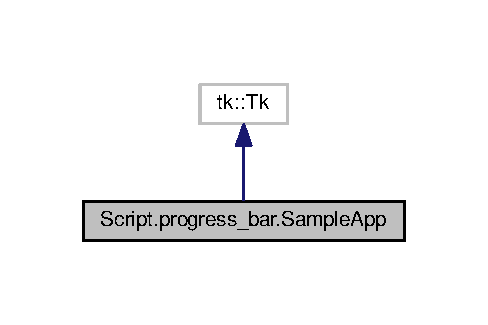
\includegraphics[width=234pt]{classScript_1_1progress__bar_1_1SampleApp__inherit__graph}
\end{center}
\end{figure}


Graphe de collaboration de Script.\+progress\+\_\+bar.\+Sample\+App\+:\nopagebreak
\begin{figure}[H]
\begin{center}
\leavevmode
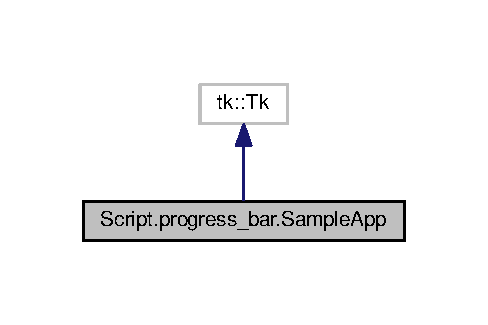
\includegraphics[width=234pt]{classScript_1_1progress__bar_1_1SampleApp__coll__graph}
\end{center}
\end{figure}
\subsection*{Fonctions membres publiques}
\begin{DoxyCompactItemize}
\item 
def \hyperlink{classScript_1_1progress__bar_1_1SampleApp_ac74edf5e4c6a6835b34e3df414954187}{\+\_\+\+\_\+init\+\_\+\+\_\+} (self, args, kwargs)
\item 
def \hyperlink{classScript_1_1progress__bar_1_1SampleApp_a9c3207958e5b061a0c5c43d986ccb17b}{start} (self)
\item 
def \hyperlink{classScript_1_1progress__bar_1_1SampleApp_ac84a187555b70009960d8205c352a6c7}{read\+\_\+bytes} (self)
\end{DoxyCompactItemize}
\subsection*{Attributs publics}
\begin{DoxyCompactItemize}
\item 
\hyperlink{classScript_1_1progress__bar_1_1SampleApp_adcc315f09b0a9f25d6e88f3b437adc47}{button}
\item 
\hyperlink{classScript_1_1progress__bar_1_1SampleApp_a355ba6fd4aa8e8bf5e29af65f8f20438}{progress}
\item 
\hyperlink{classScript_1_1progress__bar_1_1SampleApp_ae94d76abefd4f51bfcdf5cd8c7e6733b}{bytes}
\item 
\hyperlink{classScript_1_1progress__bar_1_1SampleApp_a119658b6add8ce6f70ad9f6470549fd7}{maxbytes}
\item 
\hyperlink{classScript_1_1progress__bar_1_1SampleApp_a9514fa73fb289377cbade22206b07038}{begin\+\_\+time}
\item 
\hyperlink{classScript_1_1progress__bar_1_1SampleApp_aa1283405b946ed19504ad78ef1304ddf}{end\+\_\+time}
\item 
\hyperlink{classScript_1_1progress__bar_1_1SampleApp_a13f4e7f6791df1d752e0d0e9f89c8c35}{last\+\_\+time}
\item 
\hyperlink{classScript_1_1progress__bar_1_1SampleApp_a9904e1932de17caa7610352612c2e78c}{pas}
\item 
\hyperlink{classScript_1_1progress__bar_1_1SampleApp_a89091b21cdee15376ccac1c7a2b5c887}{diff\+\_\+time}
\end{DoxyCompactItemize}


\subsection{Description détaillée}


Définition à la ligne 17 du fichier progress\+\_\+bar.\+py.



\subsection{Documentation des constructeurs et destructeur}
\mbox{\Hypertarget{classScript_1_1progress__bar_1_1SampleApp_ac74edf5e4c6a6835b34e3df414954187}\label{classScript_1_1progress__bar_1_1SampleApp_ac74edf5e4c6a6835b34e3df414954187}} 
\index{Script\+::progress\+\_\+bar\+::\+Sample\+App@{Script\+::progress\+\_\+bar\+::\+Sample\+App}!\+\_\+\+\_\+init\+\_\+\+\_\+@{\+\_\+\+\_\+init\+\_\+\+\_\+}}
\index{\+\_\+\+\_\+init\+\_\+\+\_\+@{\+\_\+\+\_\+init\+\_\+\+\_\+}!Script\+::progress\+\_\+bar\+::\+Sample\+App@{Script\+::progress\+\_\+bar\+::\+Sample\+App}}
\subsubsection{\texorpdfstring{\+\_\+\+\_\+init\+\_\+\+\_\+()}{\_\_init\_\_()}}
{\footnotesize\ttfamily def Script.\+progress\+\_\+bar.\+Sample\+App.\+\_\+\+\_\+init\+\_\+\+\_\+ (\begin{DoxyParamCaption}\item[{}]{self,  }\item[{}]{args,  }\item[{}]{kwargs }\end{DoxyParamCaption})}



Définition à la ligne 18 du fichier progress\+\_\+bar.\+py.


\begin{DoxyCode}
18     \textcolor{keyword}{def }\_\_init\_\_(self, *args, **kwargs):
19         tk.Tk.\_\_init\_\_(self, *args, **kwargs)
20         self.button = ttk.Button(text=\textcolor{stringliteral}{"start"}, command=self.start)
21         self.button.pack()
22         self.progress = ttk.Progressbar(self, orient=\textcolor{stringliteral}{"horizontal"},length=200, mode=\textcolor{stringliteral}{"determinate"})
23         self.progress.pack()
24 
25         self.bytes = 0
26         self.maxbytes = 0
27         date\_text = \textcolor{stringliteral}{"2016-07-11 15:26"}
28         date = datetime.datetime.strptime(date\_text, \textcolor{stringliteral}{"%Y-%m-%d %H:%M"})
29         print(date)
30         self.begin\_time =calendar.timegm(datetime.datetime.now().utctimetuple())
31         self.end\_time= int(calendar.timegm(date.utctimetuple()) - self.begin\_time)
32         self.last\_time=self.begin\_time
33 
34         print(self.end\_time)
35         self.pas=0
36 
37 
\end{DoxyCode}


\subsection{Documentation des fonctions membres}
\mbox{\Hypertarget{classScript_1_1progress__bar_1_1SampleApp_ac84a187555b70009960d8205c352a6c7}\label{classScript_1_1progress__bar_1_1SampleApp_ac84a187555b70009960d8205c352a6c7}} 
\index{Script\+::progress\+\_\+bar\+::\+Sample\+App@{Script\+::progress\+\_\+bar\+::\+Sample\+App}!read\+\_\+bytes@{read\+\_\+bytes}}
\index{read\+\_\+bytes@{read\+\_\+bytes}!Script\+::progress\+\_\+bar\+::\+Sample\+App@{Script\+::progress\+\_\+bar\+::\+Sample\+App}}
\subsubsection{\texorpdfstring{read\+\_\+bytes()}{read\_bytes()}}
{\footnotesize\ttfamily def Script.\+progress\+\_\+bar.\+Sample\+App.\+read\+\_\+bytes (\begin{DoxyParamCaption}\item[{}]{self }\end{DoxyParamCaption})}



Définition à la ligne 45 du fichier progress\+\_\+bar.\+py.



Référencé par Script.\+progress\+\_\+bar.\+Sample\+App.\+start().


\begin{DoxyCode}
45     \textcolor{keyword}{def }read\_bytes(self):
46 
47         self.diff\_time= calendar.timegm(datetime.datetime.now().utctimetuple())
48         self.bytes += int(self.diff\_time - self.last\_time)
49         self.last\_time= self.diff\_time
50         self.progress[\textcolor{stringliteral}{"value"}] = self.bytes
51 
52         self.pas= int(self.diff\_time - self.begin\_time)
53         print(self.pas)
54         pourcentage= round((self.pas*100) / self.end\_time)
55         print(str(pourcentage));
56 
57         
58         \textcolor{keywordflow}{if} self.bytes < self.maxbytes:
59             self.after(100, self.read\_bytes)
60 
61 
\end{DoxyCode}
Voici le graphe des appelants de cette fonction \+:\nopagebreak
\begin{figure}[H]
\begin{center}
\leavevmode
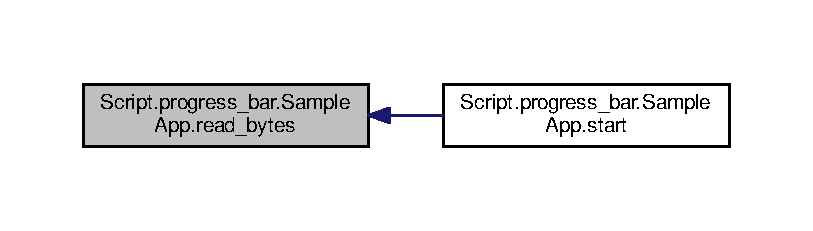
\includegraphics[width=350pt]{classScript_1_1progress__bar_1_1SampleApp_ac84a187555b70009960d8205c352a6c7_icgraph}
\end{center}
\end{figure}
\mbox{\Hypertarget{classScript_1_1progress__bar_1_1SampleApp_a9c3207958e5b061a0c5c43d986ccb17b}\label{classScript_1_1progress__bar_1_1SampleApp_a9c3207958e5b061a0c5c43d986ccb17b}} 
\index{Script\+::progress\+\_\+bar\+::\+Sample\+App@{Script\+::progress\+\_\+bar\+::\+Sample\+App}!start@{start}}
\index{start@{start}!Script\+::progress\+\_\+bar\+::\+Sample\+App@{Script\+::progress\+\_\+bar\+::\+Sample\+App}}
\subsubsection{\texorpdfstring{start()}{start()}}
{\footnotesize\ttfamily def Script.\+progress\+\_\+bar.\+Sample\+App.\+start (\begin{DoxyParamCaption}\item[{}]{self }\end{DoxyParamCaption})}



Définition à la ligne 39 du fichier progress\+\_\+bar.\+py.



Références Script.\+progress\+\_\+bar.\+Sample\+App.\+end\+\_\+time, Script.\+progress\+\_\+bar.\+Sample\+App.\+maxbytes, Script.\+progress\+\_\+bar.\+Sample\+App.\+progress, et Script.\+progress\+\_\+bar.\+Sample\+App.\+read\+\_\+bytes().


\begin{DoxyCode}
39     \textcolor{keyword}{def }start(self):
40         self.progress[\textcolor{stringliteral}{"value"}] = 0
41         self.maxbytes = self.end\_time
42         self.progress[\textcolor{stringliteral}{"maximum"}] = self.end\_time
43         self.read\_bytes()
44 
\end{DoxyCode}
Voici le graphe d\textquotesingle{}appel pour cette fonction \+:\nopagebreak
\begin{figure}[H]
\begin{center}
\leavevmode
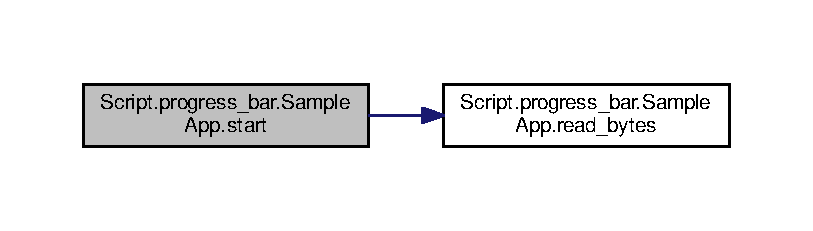
\includegraphics[width=350pt]{classScript_1_1progress__bar_1_1SampleApp_a9c3207958e5b061a0c5c43d986ccb17b_cgraph}
\end{center}
\end{figure}


\subsection{Documentation des données membres}
\mbox{\Hypertarget{classScript_1_1progress__bar_1_1SampleApp_a9514fa73fb289377cbade22206b07038}\label{classScript_1_1progress__bar_1_1SampleApp_a9514fa73fb289377cbade22206b07038}} 
\index{Script\+::progress\+\_\+bar\+::\+Sample\+App@{Script\+::progress\+\_\+bar\+::\+Sample\+App}!begin\+\_\+time@{begin\+\_\+time}}
\index{begin\+\_\+time@{begin\+\_\+time}!Script\+::progress\+\_\+bar\+::\+Sample\+App@{Script\+::progress\+\_\+bar\+::\+Sample\+App}}
\subsubsection{\texorpdfstring{begin\+\_\+time}{begin\_time}}
{\footnotesize\ttfamily Script.\+progress\+\_\+bar.\+Sample\+App.\+begin\+\_\+time}



Définition à la ligne 30 du fichier progress\+\_\+bar.\+py.

\mbox{\Hypertarget{classScript_1_1progress__bar_1_1SampleApp_adcc315f09b0a9f25d6e88f3b437adc47}\label{classScript_1_1progress__bar_1_1SampleApp_adcc315f09b0a9f25d6e88f3b437adc47}} 
\index{Script\+::progress\+\_\+bar\+::\+Sample\+App@{Script\+::progress\+\_\+bar\+::\+Sample\+App}!button@{button}}
\index{button@{button}!Script\+::progress\+\_\+bar\+::\+Sample\+App@{Script\+::progress\+\_\+bar\+::\+Sample\+App}}
\subsubsection{\texorpdfstring{button}{button}}
{\footnotesize\ttfamily Script.\+progress\+\_\+bar.\+Sample\+App.\+button}



Définition à la ligne 20 du fichier progress\+\_\+bar.\+py.

\mbox{\Hypertarget{classScript_1_1progress__bar_1_1SampleApp_ae94d76abefd4f51bfcdf5cd8c7e6733b}\label{classScript_1_1progress__bar_1_1SampleApp_ae94d76abefd4f51bfcdf5cd8c7e6733b}} 
\index{Script\+::progress\+\_\+bar\+::\+Sample\+App@{Script\+::progress\+\_\+bar\+::\+Sample\+App}!bytes@{bytes}}
\index{bytes@{bytes}!Script\+::progress\+\_\+bar\+::\+Sample\+App@{Script\+::progress\+\_\+bar\+::\+Sample\+App}}
\subsubsection{\texorpdfstring{bytes}{bytes}}
{\footnotesize\ttfamily Script.\+progress\+\_\+bar.\+Sample\+App.\+bytes}



Définition à la ligne 25 du fichier progress\+\_\+bar.\+py.

\mbox{\Hypertarget{classScript_1_1progress__bar_1_1SampleApp_a89091b21cdee15376ccac1c7a2b5c887}\label{classScript_1_1progress__bar_1_1SampleApp_a89091b21cdee15376ccac1c7a2b5c887}} 
\index{Script\+::progress\+\_\+bar\+::\+Sample\+App@{Script\+::progress\+\_\+bar\+::\+Sample\+App}!diff\+\_\+time@{diff\+\_\+time}}
\index{diff\+\_\+time@{diff\+\_\+time}!Script\+::progress\+\_\+bar\+::\+Sample\+App@{Script\+::progress\+\_\+bar\+::\+Sample\+App}}
\subsubsection{\texorpdfstring{diff\+\_\+time}{diff\_time}}
{\footnotesize\ttfamily Script.\+progress\+\_\+bar.\+Sample\+App.\+diff\+\_\+time}



Définition à la ligne 47 du fichier progress\+\_\+bar.\+py.

\mbox{\Hypertarget{classScript_1_1progress__bar_1_1SampleApp_aa1283405b946ed19504ad78ef1304ddf}\label{classScript_1_1progress__bar_1_1SampleApp_aa1283405b946ed19504ad78ef1304ddf}} 
\index{Script\+::progress\+\_\+bar\+::\+Sample\+App@{Script\+::progress\+\_\+bar\+::\+Sample\+App}!end\+\_\+time@{end\+\_\+time}}
\index{end\+\_\+time@{end\+\_\+time}!Script\+::progress\+\_\+bar\+::\+Sample\+App@{Script\+::progress\+\_\+bar\+::\+Sample\+App}}
\subsubsection{\texorpdfstring{end\+\_\+time}{end\_time}}
{\footnotesize\ttfamily Script.\+progress\+\_\+bar.\+Sample\+App.\+end\+\_\+time}



Définition à la ligne 31 du fichier progress\+\_\+bar.\+py.



Référencé par Script.\+progress\+\_\+bar.\+Sample\+App.\+start().

\mbox{\Hypertarget{classScript_1_1progress__bar_1_1SampleApp_a13f4e7f6791df1d752e0d0e9f89c8c35}\label{classScript_1_1progress__bar_1_1SampleApp_a13f4e7f6791df1d752e0d0e9f89c8c35}} 
\index{Script\+::progress\+\_\+bar\+::\+Sample\+App@{Script\+::progress\+\_\+bar\+::\+Sample\+App}!last\+\_\+time@{last\+\_\+time}}
\index{last\+\_\+time@{last\+\_\+time}!Script\+::progress\+\_\+bar\+::\+Sample\+App@{Script\+::progress\+\_\+bar\+::\+Sample\+App}}
\subsubsection{\texorpdfstring{last\+\_\+time}{last\_time}}
{\footnotesize\ttfamily Script.\+progress\+\_\+bar.\+Sample\+App.\+last\+\_\+time}



Définition à la ligne 32 du fichier progress\+\_\+bar.\+py.

\mbox{\Hypertarget{classScript_1_1progress__bar_1_1SampleApp_a119658b6add8ce6f70ad9f6470549fd7}\label{classScript_1_1progress__bar_1_1SampleApp_a119658b6add8ce6f70ad9f6470549fd7}} 
\index{Script\+::progress\+\_\+bar\+::\+Sample\+App@{Script\+::progress\+\_\+bar\+::\+Sample\+App}!maxbytes@{maxbytes}}
\index{maxbytes@{maxbytes}!Script\+::progress\+\_\+bar\+::\+Sample\+App@{Script\+::progress\+\_\+bar\+::\+Sample\+App}}
\subsubsection{\texorpdfstring{maxbytes}{maxbytes}}
{\footnotesize\ttfamily Script.\+progress\+\_\+bar.\+Sample\+App.\+maxbytes}



Définition à la ligne 26 du fichier progress\+\_\+bar.\+py.



Référencé par Script.\+progress\+\_\+bar.\+Sample\+App.\+start().

\mbox{\Hypertarget{classScript_1_1progress__bar_1_1SampleApp_a9904e1932de17caa7610352612c2e78c}\label{classScript_1_1progress__bar_1_1SampleApp_a9904e1932de17caa7610352612c2e78c}} 
\index{Script\+::progress\+\_\+bar\+::\+Sample\+App@{Script\+::progress\+\_\+bar\+::\+Sample\+App}!pas@{pas}}
\index{pas@{pas}!Script\+::progress\+\_\+bar\+::\+Sample\+App@{Script\+::progress\+\_\+bar\+::\+Sample\+App}}
\subsubsection{\texorpdfstring{pas}{pas}}
{\footnotesize\ttfamily Script.\+progress\+\_\+bar.\+Sample\+App.\+pas}



Définition à la ligne 35 du fichier progress\+\_\+bar.\+py.

\mbox{\Hypertarget{classScript_1_1progress__bar_1_1SampleApp_a355ba6fd4aa8e8bf5e29af65f8f20438}\label{classScript_1_1progress__bar_1_1SampleApp_a355ba6fd4aa8e8bf5e29af65f8f20438}} 
\index{Script\+::progress\+\_\+bar\+::\+Sample\+App@{Script\+::progress\+\_\+bar\+::\+Sample\+App}!progress@{progress}}
\index{progress@{progress}!Script\+::progress\+\_\+bar\+::\+Sample\+App@{Script\+::progress\+\_\+bar\+::\+Sample\+App}}
\subsubsection{\texorpdfstring{progress}{progress}}
{\footnotesize\ttfamily Script.\+progress\+\_\+bar.\+Sample\+App.\+progress}



Définition à la ligne 22 du fichier progress\+\_\+bar.\+py.



Référencé par Script.\+progress\+\_\+bar.\+Sample\+App.\+start().



La documentation de cette classe a été générée à partir du fichier suivant \+:\begin{DoxyCompactItemize}
\item 
\hyperlink{progress__bar_8py}{progress\+\_\+bar.\+py}\end{DoxyCompactItemize}

\chapter{Documentation des fichiers}
\hypertarget{____init_____8py}{}\section{Référence du fichier \+\_\+\+\_\+init\+\_\+\+\_\+.\+py}
\label{____init_____8py}\index{\+\_\+\+\_\+init\+\_\+\+\_\+.\+py@{\+\_\+\+\_\+init\+\_\+\+\_\+.\+py}}
\subsection*{Espaces de nommage}
\begin{DoxyCompactItemize}
\item 
 \hyperlink{namespaceScript}{Script}
\end{DoxyCompactItemize}

\hypertarget{handOver_8py}{}\section{Référence du fichier hand\+Over.\+py}
\label{handOver_8py}\index{hand\+Over.\+py@{hand\+Over.\+py}}
\subsection*{Classes}
\begin{DoxyCompactItemize}
\item 
class \hyperlink{classScript_1_1handOver_1_1MobileReceives}{Script.\+hand\+Over.\+Mobile\+Receives}
\item 
class \hyperlink{classScript_1_1handOver_1_1MobileTransmitter}{Script.\+hand\+Over.\+Mobile\+Transmitter}
\end{DoxyCompactItemize}
\subsection*{Espaces de nommage}
\begin{DoxyCompactItemize}
\item 
 \hyperlink{namespaceScript_1_1handOver}{Script.\+hand\+Over}
\end{DoxyCompactItemize}
\subsection*{Fonctions}
\begin{DoxyCompactItemize}
\item 
def \hyperlink{namespaceScript_1_1handOver_a4d9a0e646528d168d925b4bcd6f078a6}{Script.\+hand\+Over.\+begin\+\_\+hand\+Over} (simple, tmu, ptp, data, vgcs, rec, vbs)
\end{DoxyCompactItemize}
\subsection*{Variables}
\begin{DoxyCompactItemize}
\item 
\hyperlink{namespaceScript_1_1handOver_a94f94a457b98f7aa4528c5118490f262}{Script.\+hand\+Over.\+V\+E\+R\+R\+OU} = R\+Lock()
\item 
bool \hyperlink{namespaceScript_1_1handOver_a1f8a11e1df500a2ab144549e8f3e4703}{Script.\+hand\+Over.\+C\+O\+N\+F\+I\+RM} = True
\item 
int \hyperlink{namespaceScript_1_1handOver_a10996755a745f6ffa98a8c5235d8d4b3}{Script.\+hand\+Over.\+baudrate} = 9600
\end{DoxyCompactItemize}

\hypertarget{interfaceFrame_8py}{}\section{Référence du fichier interface\+Frame.\+py}
\label{interfaceFrame_8py}\index{interface\+Frame.\+py@{interface\+Frame.\+py}}
\subsection*{Espaces de nommage}
\begin{DoxyCompactItemize}
\item 
 \hyperlink{namespaceScript_1_1interfaceFrame}{Script.\+interface\+Frame}
\end{DoxyCompactItemize}
\subsection*{Fonctions}
\begin{DoxyCompactItemize}
\item 
def \hyperlink{namespaceScript_1_1interfaceFrame_aa7f559f2c9e8af048daa456cb3686155}{Script.\+interface\+Frame.\+Frame\+\_\+init\+\_\+option} (self, other\+Frame2, other\+Frame3)
\item 
def \hyperlink{namespaceScript_1_1interfaceFrame_a3538cb8357b74776a380240ed3221bc0}{Script.\+interface\+Frame.\+Frame\+\_\+select\+\_\+com} (self, val\+\_\+type)
\item 
def \hyperlink{namespaceScript_1_1interfaceFrame_ae94a2df22674070fddf2ae5197a09a6f}{Script.\+interface\+Frame.\+Frame\+\_\+btn\+\_\+execution} (self)
\item 
def \hyperlink{namespaceScript_1_1interfaceFrame_a76119121c3aceb43846ba3ea526623ad}{Script.\+interface\+Frame.\+Scan\+\_\+com} ()
\item 
def \hyperlink{namespaceScript_1_1interfaceFrame_a7a90dd83e0b67edcf2dee870d927e98e}{Script.\+interface\+Frame.\+verif\+\_\+args} ()
\item 
def \hyperlink{namespaceScript_1_1interfaceFrame_ab554e77db5080fb2eae78e39ebbeb395}{Script.\+interface\+Frame.\+split\+\_\+chaine} (chaine, caractere)
\end{DoxyCompactItemize}
\subsection*{Variables}
\begin{DoxyCompactItemize}
\item 
\hyperlink{namespaceScript_1_1interfaceFrame_ab8e385a4d6a1f87628b963bc0a385519}{Script.\+interface\+Frame.\+begin\+\_\+time} = time.\+time()
\item 
int \hyperlink{namespaceScript_1_1interfaceFrame_ace1207561541cc3ee3af9b2f33b2a316}{Script.\+interface\+Frame.\+val\+\_\+line} = 0
\item 
string \hyperlink{namespaceScript_1_1interfaceFrame_a2cfacdb24b52e8cf5d9667d91a5c58ab}{Script.\+interface\+Frame.\+V\+A\+L\+U\+E\+\_\+\+F\+I\+L\+E\+\_\+\+C\+O\+NF} = \char`\"{}\char`\"{}
\item 
string \hyperlink{namespaceScript_1_1interfaceFrame_a3704b57444e587c904b839d2dfef2b7e}{Script.\+interface\+Frame.\+V\+A\+L\+U\+E\+\_\+\+F\+I\+L\+E\+\_\+\+C\+MD} = \char`\"{}\char`\"{}
\item 
string \hyperlink{namespaceScript_1_1interfaceFrame_a8933d662775f7e5fc3e0b8e5fb499b24}{Script.\+interface\+Frame.\+V\+A\+L\+U\+E\+\_\+\+F\+I\+L\+E\+\_\+\+S\+A\+VE} = \char`\"{}\char`\"{}
\item 
string \hyperlink{namespaceScript_1_1interfaceFrame_a235ac21d18cefa672100db29db0ed490}{Script.\+interface\+Frame.\+V\+A\+L\+U\+E\+\_\+\+F\+I\+L\+E\+\_\+\+A\+U\+D\+IO} = \char`\"{}\char`\"{}
\end{DoxyCompactItemize}

\hypertarget{omc_8py}{}\section{Référence du fichier omc.\+py}
\label{omc_8py}\index{omc.\+py@{omc.\+py}}
\subsection*{Classes}
\begin{DoxyCompactItemize}
\item 
class \hyperlink{classScript_1_1omc_1_1OMC}{Script.\+omc.\+O\+MC}
\end{DoxyCompactItemize}
\subsection*{Espaces de nommage}
\begin{DoxyCompactItemize}
\item 
 \hyperlink{namespaceScript_1_1omc}{Script.\+omc}
\end{DoxyCompactItemize}

\hypertarget{omu_8py}{}\section{Référence du fichier omu.\+py}
\label{omu_8py}\index{omu.\+py@{omu.\+py}}
\subsection*{Classes}
\begin{DoxyCompactItemize}
\item 
class \hyperlink{classScript_1_1omu_1_1OMU}{Script.\+omu.\+O\+MU}
\end{DoxyCompactItemize}
\subsection*{Espaces de nommage}
\begin{DoxyCompactItemize}
\item 
 \hyperlink{namespaceScript_1_1omu}{Script.\+omu}
\end{DoxyCompactItemize}

\hypertarget{Option_8py}{}\section{Référence du fichier Option.\+py}
\label{Option_8py}\index{Option.\+py@{Option.\+py}}
\subsection*{Espaces de nommage}
\begin{DoxyCompactItemize}
\item 
 \hyperlink{namespaceScript_1_1Option}{Script.\+Option}
\end{DoxyCompactItemize}
\subsection*{Fonctions}
\begin{DoxyCompactItemize}
\item 
def \hyperlink{namespaceScript_1_1Option_abb674ebac6565861fc8240a9306f8ecd}{Script.\+Option.\+callback\+\_\+quit} ()
\item 
def \hyperlink{namespaceScript_1_1Option_aff91639f98fde0463987ea08e565da05}{Script.\+Option.\+progress\+\_\+\+Bar} ()
\item 
def \hyperlink{namespaceScript_1_1Option_a09506d9cf0343fc80883c5db0a207737}{Script.\+Option.\+save\+\_\+\+Data} (my\+\_\+object)
\item 
def \hyperlink{namespaceScript_1_1Option_ac71533bc42f23543f3c564ccf01d9faf}{Script.\+Option.\+split\+\_\+chaine} (chaine, caractere)
\item 
def \hyperlink{namespaceScript_1_1Option_a1707d1e8b288159100845df330fc8d51}{Script.\+Option.\+limit\+\_\+waiting} ()
\item 
def \hyperlink{namespaceScript_1_1Option_a22c03fd81ddb28ef13f194565b4996ba}{Script.\+Option.\+hang\+\_\+up\+\_\+call} (phone)
\end{DoxyCompactItemize}

\hypertarget{progress__bar_8py}{}\section{Référence du fichier progress\+\_\+bar.\+py}
\label{progress__bar_8py}\index{progress\+\_\+bar.\+py@{progress\+\_\+bar.\+py}}
\subsection*{Classes}
\begin{DoxyCompactItemize}
\item 
class \hyperlink{classScript_1_1progress__bar_1_1SampleApp}{Script.\+progress\+\_\+bar.\+Sample\+App}
\end{DoxyCompactItemize}
\subsection*{Espaces de nommage}
\begin{DoxyCompactItemize}
\item 
 \hyperlink{namespaceScript_1_1progress__bar}{Script.\+progress\+\_\+bar}
\end{DoxyCompactItemize}
\subsection*{Variables}
\begin{DoxyCompactItemize}
\item 
\hyperlink{namespaceScript_1_1progress__bar_a2346ccb846bab632249778f76d43e342}{Script.\+progress\+\_\+bar.\+app} = Sample\+App()
\end{DoxyCompactItemize}

\hypertarget{Setup_8py}{}\section{Référence du fichier Setup.\+py}
\label{Setup_8py}\index{Setup.\+py@{Setup.\+py}}
\subsection*{Classes}
\begin{DoxyCompactItemize}
\item 
class \hyperlink{classScript_1_1Setup_1_1MainInterface}{Script.\+Setup.\+Main\+Interface}
\end{DoxyCompactItemize}
\subsection*{Espaces de nommage}
\begin{DoxyCompactItemize}
\item 
 \hyperlink{namespaceScript_1_1Setup}{Script.\+Setup}
\end{DoxyCompactItemize}
\subsection*{Variables}
\begin{DoxyCompactItemize}
\item 
\hyperlink{namespaceScript_1_1Setup_a29d68f31a39926032c0d32fe3ea0c4eb}{Script.\+Setup.\+fenetre} = Tk()
\item 
\hyperlink{namespaceScript_1_1Setup_a430ab18615fdd48075635baef7ed6832}{Script.\+Setup.\+width}
\item 
\hyperlink{namespaceScript_1_1Setup_a21f36134f509add0c0704c2ed5ea51fc}{Script.\+Setup.\+False}
\item 
\hyperlink{namespaceScript_1_1Setup_a334aa187cc8c0b7354d8f6b33894d575}{Script.\+Setup.\+height}
\item 
\hyperlink{namespaceScript_1_1Setup_a11f256776bccf507b8e83363360c8ff7}{Script.\+Setup.\+interface} = Main\+Interface(fenetre)
\end{DoxyCompactItemize}

%--- End generated contents ---

% Index
\backmatter
\newpage
\phantomsection
\clearemptydoublepage
\addcontentsline{toc}{chapter}{Index}
\printindex

\end{document}
